\documentclass[
    chapter=TITLE,
    12pt, 		% Tamanho da fonte
    openright,% Capítulos começam em pág. ímpar (insere página vazia caso preciso)
    oneside, 	% Para impressão somente verso. Oposto a impressão em verso e anverso
    a4paper, 	% Tamanho do papel
    english, 	% Idioma adicional para hifenização
    brazil 		% o último idioma é o principal do documento
    ]{abntex2}
    
\usepackage[utf8]{inputenc}
\usepackage{tikz}
\usepackage{wrapfig}
\usetikzlibrary{calc}
\usepackage{lipsum} 	% para geração de dummy text
\usepackage{multirow}

% Pacotes
%% Sumário
\usepackage{tocloft}

%% Codificação
\usepackage[T1]{fontenc} 	% Codificação de saída

%% Fonte
\usepackage{times} 			% Times New Roman

\usepackage{lastpage} 		% Usado pela Ficha catalográfica
\usepackage{indentfirst} 	% Indenta o primeiro parágrafo de cada seção.
\usepackage{color} 				% Controle das cores
\usepackage{microtype} 		% Para melhorias de justificação
\usepackage{lscape} 			% Permite a criação de conteúdo em modo paisagem
\usepackage{hyperref} 		% Criação de links
\usepackage{etoolbox}

%% Tabelas
\usepackage{multirow}

%% Sumário
\usepackage{textcase}

%% Imagens
\usepackage{graphicx} % Inclusão de gráficos

%% Tamanho e alinhamento das legendas
\usepackage[
	singlelinecheck=false,
	justification=justified,
	font=footnotesize
	]
	{caption}

%% Citações
\usepackage[hyphenbreaks]{breakurl}
\usepackage[alf,abnt-emphasize=em]{abntex2cite}

\renewcommand
	{\familydefault}
	{\sfdefault} 			% Seta fonte default

%% Redefine booleans
%\setboolean{ABNTEXuppersubsection}{false}

%% Cabeçalho padrao
\makepagestyle
	{abntheadings}
\makeevenhead
	{abntheadings}
	{\ABNTEXfontereduzida\thepage}
	{}
	{\ABNTEXfontereduzida\textit\leftmark}
\makeoddhead
	{abntheadings}
	{}
	{}
	{\ABNTEXfontereduzida\thepage}
\makeheadrule
	{abntheadings}
	{0pt}
	{\normalrulethickness}

%% Cabeçalho do inicio do capitulo
\makepagestyle
	{abntchapfirst}
\makeoddhead
	{abntchapfirst}
	{}
	{}
	{\ABNTEXfontereduzida\thepage}


% Estilos
\autor{Vítor Gavião Lima Januario} 	%Nome do autor
% Especificidades para a entrada de autor pessoal: – sobrenome com indicativo de parentesco
% Quando o autor é brasileiro, trate o grau de parentesco como parte do sobrenome.
% Exemplo: Autor: Luís Fernando Carvalho Neto - Entrada: CARVALHO NETO, L. F.
\newcommand{\entradaAutor}{JANUARIO, V. G. L} % Sem ponto no final
% Titulo do trabalho
\titulo{Aplicativo colaborativo para compra inteligente de produtos em comércio
local} %Título do trabalho
\newcommand{\englishTitle}{Collaborative mobile application for smart purchase of products in local commerce}
\data{\today}			%Ano de publicação
\local{Nova Friburgo}	%Local
%% Membros da banca
\newcommand{\membrobancaA}{}
\newcommand{\membrobancaB}{}
\newcommand{\membrobancaC}{}

\providecommand
	{\imprimirmembrobancaA}
	{}
\providecommand
	{\imprimirmembrobancaAinst}
	{}
\renewcommand
	{\membrobancaA}
	[2]
	[\imprimirinstituicao]
	{\renewcommand
		{\imprimirmembrobancaA}
		{#2}
		\renewcommand
		{\imprimirmembrobancaAinst}
		{#1}
	}

\providecommand
	{\imprimirmembrobancaB}
	{}
\providecommand
	{\imprimirmembrobancaBinst}
	{}
\renewcommand
	{\membrobancaB}
	[2]
	[\imprimirinstituicao]
	{
		\renewcommand
		{\imprimirmembrobancaB}
		{#2}
		\renewcommand
		{\imprimirmembrobancaBinst}
		{#1}
	}

\providecommand
	{\imprimirmembrobancaC}
	{}
\providecommand
	{\imprimirmembrobancaCinst}
	{}
\renewcommand
	{\membrobancaC}
	[2]
	[\imprimirinstituicao]
	{
		\renewcommand
		{\imprimirmembrobancaC}
		{#2}
		\renewcommand
		{\imprimirmembrobancaCinst}
		{#1}
	}

\newcommand
	{\imprimirmeOrientadorinst}
	{\imprimirinstituicao}
\newcommand
	{\imprimirmeCoorientadorinst}
	{\imprimirinstituicao}

%% Natureza do trabalho
\providecommand{\imprimirnaturezatrabalho}{}
\newcommand{\naturezatrabalho}[1]{
	\renewcommand{\imprimirnaturezatrabalho}{#1}
}

%% Redefinir resumo
\renewenvironment{resumo}[1][\resumoname]{%
	\pretextualchapter{#1}
}{\PRIVATEclearpageifneeded}

%% Redefinir dedicatória
\renewenvironment{dedicatoria}[1][]
{
	\ifthenelse{\equal{#1}{}}{
		\PRIVATEbookmarkthis{\dedicatorianame}
	}{\preamblealchapter{#1}}
	
	\vspace*{\fill}
}
{}

\renewenvironment{epigrafe}[1][]
{
	\ifthenelse{\equal{#1}{}}{
		\PRIVATEbookmarkthis{\epigraphname}
	}{\pretextualchapter{#1}}
	
	\vspace*{\fill}
}
{
	
}

%% Comando para inserir sigla
\newcommand{\sigla}[2][]{
	\item[#1] \textit{#2}
}

%% Redefinição da formatação do \chapter
\renewcommand{\ABNTEXchapterfont}{\normalfont\fontseries{b}\selectfont}
\renewcommand{\ABNTEXchapterfontsize}{\normalsize}
\renewcommand{\ABNTEXpartfont}{\fontseries{b}\selectfont\selectfont}
\renewcommand{\ABNTEXpartfontsize}{\normalsize}
\renewcommand{\ABNTEXsectionfont}{\normalfont\selectfont} %\fontseries{b}
\renewcommand{\ABNTEXsectionfontsize}{\normalsize}
\renewcommand{\ABNTEXsubsectionfont}{\normalfont}
\renewcommand{\ABNTEXsubsectionfontsize}{\normalsize}
\renewcommand{\ABNTEXsubsubsectionfont}{\normalfont}
\renewcommand{\ABNTEXsubsubsectionfontsize}{\normalsize}
\renewcommand{\ABNTEXsubsubsubsectionfont}{\normalfont}
\renewcommand{\ABNTEXsubsubsubsectionfontsize}{\normalsize}
%\renewcommand{\ABNTEXsubsubsectionfont}{\normalfont\fontseries{b}\selectfont}
%\renewcommand{\ABNTEXsubsubsectionfontsize}{\normalsize}
%\renewcommand{\ABNTEXsubsubsubsectionfont}{\normalfont\itshape\selectfont}
%\renewcommand{\ABNTEXsubsubsubsectionfontsize}{\normalsize}



%% Redefinição da formatação de Parágrafos 
\setlength{\parindent}{1.3cm}
\setlength{\parskip}{0cm}

%% Sumário
\makeatletter
\addtocontents{toc}{%
	\protect\renewcommand{\protect\cftchapterleader}{%-- switch it on here
		\normalsize\normalfont\protect\cftdotfill{\protect\cftdotsep}}}
\renewcommand{\cftchapterpresnum}{\normalfont} % Numeração do capítulo não ficar em negrito
\renewcommand{\cftchapterpagefont}{\normalfont} % Páginas do capítulo não ficar em negrito
\renewcommand*{\cftchapterfont}{\normalfont\bfseries} % Título do capítulo em negrito
\renewcommand{\chapnumfont}{\normalfont\normalsize}
\renewcommand*{\cftsectionfont}{\normalfont} %\fontseries{b}
\renewcommand*{\cftsubsectionfont}{\normalfont}
\renewcommand*{\cftsubsubsectionfont}{\normalfont}
\renewcommand*{\cftsubsubsubsectionfont}{\normalfont}
\renewcommand*{\cftparagraphfont}{\normalfont} %\itshape



%% Forca underline na secao terciaria
\newcommand{\tmpsubsection}[1]{}
\let\tmpsubsection=\subsection
\renewcommand{\subsection}[1]{\tmpsubsection{\underline{#1}}}

%% Forca underline na secao secundaroa
\newcommand{\tmpsection}[1]{}
\let\tmpsection=\section
\renewcommand{\section}[1]{\tmpsection{\textbf{#1}}}
\makeatother
%% Tornar as seções secundários com fonte em maiúscula
%\makeatletter
%\let\oldcontentsline\contentsline
%\def\contentsline#1#2{%
%  \expandafter\ifx\csname l@#1\endcsname\l@section
%    \expandafter\@firstoftwo
%  \else
%    \expandafter\@secondoftwo
%  \fi
%  {%
%    \oldcontentsline{#1}{\MakeTextUppercase{#2}}%
%  }{%
%    \oldcontentsline{#1}{#2}%
%  }%
%}
%\makeatother

%% Tornar a entrada "Referências" com fonte em maiúscula
%%\addto\captionsbrazil{
%%    \renewcommand{\bibname}{REFER\^ENCIAS}
%%}

% Legendas
\makeatletter
\patchcmd{\caption@@@make}
{\ifcaption@star}
{\ifcaption@star\small}
{}{}
\makeatother


\graphicspath{ {figures/} }


\preambulo{
	Trabalho de conclusão de curso apresentado como pré-requisito para obtenção do título de Engenheiro de Computação, ao Departamento de Modelagem Computacional, do Instituto Politécnico, da Universidade do Estado do Rio de Janeiro.
}
\orientador{Prof. Dr. Bernardo Sotto-Maior Peralva}
\tipotrabalho{monografia}		%Define as configurações do arquivo

\begin{document}
	%Capa
	\renewcommand{\imprimircapa}{%
	\begin{center}
		\begin{tikzpicture}[remember picture, overlay]
		\draw[line width = 4pt] ($(current page.north west) + (20mm, -20mm)$) rectangle ($(current page.south east) + (-10mm,10mm)$);
		\draw[line width = 1pt] ($(current page.north west) + (21.5mm,-21.5mm)$) rectangle ($(current page.south east) + (-11.5mm,11.5mm)$);
		\end{tikzpicture}
		\begin{capa}
			\begin{minipage}[r]{0.1\linewidth}
				
\includegraphics[width=1.5\linewidth]{uerj} 
			\end{minipage}%
			\begin{minipage}[c]{0.7\linewidth}
				\begin{center}
					\textbf{UNIVERSIDADE DO ESTADO DO \\ RIO DE JANEIRO}\\
					\noindent\rule{7cm}{0.4pt}\\
					\textbf{INSTITUTO POLITÉCNICO \\ GRADUAÇÃO EM ENGENHARIA \\DE COMPUTAÇÃO}\\
				\end{center}
			\end{minipage}%
			\begin{minipage}[c]{0.1\linewidth}
				
\includegraphics[width=1.5\linewidth]{iprj} 
			\end{minipage}
			
			\vspace*{4.5cm}
			\center
			\textbf{\large\imprimirautor}
			\vspace*{3cm}
			\begin{center}
				\bfseries\LARGE\imprimirtitulo
			\end{center}
			\vfill
			\textbf{
				\large\imprimirlocal
				\\	
				\large \the\year
			}
			\vspace*{1cm}
		\end{capa}
	\end{center}
}
\imprimircapa
	
	%Folha de rosto
	\makeatletter
\renewcommand{\folhaderostocontent}{
	\begin{center}
		\begin{tikzpicture}[remember picture, overlay]
		\draw[line width = 4pt] ($(current page.north west) + (20mm, -20mm)$) rectangle ($(current page.south east) + (-10mm,10mm)$);
		\draw[line width = 1pt] ($(current page.north west) + (21.5mm,-21.5mm)$) rectangle ($(current page.south east) + (-11.5mm,11.5mm)$);
		\end{tikzpicture}
		
		\begin{minipage}[r]{0.1\linewidth}
			
\includegraphics[width=1.5\linewidth]{uerj} 
		\end{minipage}%
		\begin{minipage}[c]{0.7\linewidth}
			\begin{center}
				\textbf{UNIVERSIDADE DO ESTADO DO \\ RIO DE JANEIRO}\\
				\noindent\rule{7cm}{0.4pt}\\
				\textbf{INSTITUTO POLITÉCNICO \\ GRADUAÇÃO EM ENGENHARIA \\DE COMPUTAÇÃO}\\
			\end{center}
		\end{minipage}%
		\begin{minipage}[c]{0.1\linewidth}
			
\includegraphics[width=1.5\linewidth]{iprj} 
		\end{minipage}
		\vspace*{2cm}
		\begin{center}
			{\large\imprimirautor}
			\vspace*{\fill}\vspace*{\fill}
			\begin{center}
				\textbf{\large\imprimirtitulo}
			\end{center}
			\vspace*{\fill}
			\abntex@ifnotempty{\imprimirpreambulo}{%
				\hspace{.45\textwidth}
				\begin{minipage}{.5\textwidth}
					\SingleSpacing
					\imprimirpreambulo
				\end{minipage}%
				\vspace*{2cm}
				\vspace*{\fill}
			}%
			{\abntex@ifnotempty{\imprimirinstituicao}{\imprimirinstituicao
					\vspace*{\fill}}}
			{\large\imprimirorientadorRotulo~\imprimirorientador\par}
			\abntex@ifnotempty{\imprimircoorientador}{%
				{\large\imprimircoorientadorRotulo~\imprimircoorientador}%
			}%
			\vspace*{\fill}
			{\large\imprimirlocal}
			\par
			{\large\the\year}
			\vspace*{1cm}
		\end{center}	
	\end{center}
}
\makeatother
	\imprimirfolhaderosto
	
	%Catalogação Biblioteca
	\newcommand{\imprimircatalogacao}{%
	\noindent
	UNIVERSIDADE DO ESTADO DO RIO DE JANEIRO\\
	INSTITUTO POLITÉCNICO - CURSO DE ENGENHARIA DE COMPUTAÇÃO\\
	
	\noindent
	Reitor: Ruy Garcia Marques\\
	Vice-Reitor: Maria Georgina Muniz Washington\\
	Diretor do Instituto Politécnico: Ricardo Carvalho de Barros\\
	Coordenador de Curso: José Humberto Zani\\
	
	\noindent
	Banca Avaliadora Composta por: \imprimirorientador~(Orientador)\\
	\hspace*{6.3cm}Prof. Dr. Roberto Domingos Pinheiro\\
	\hspace*{6.3cm}Prof. Dr. Anderson Amendoeira Namen
	
	\begin{center}
		CATALOGAÇÃO NA FONTE \\ UERJ/REDE SIRIUS/BIBLIOTECA CTC/E
		\end{center}
		\begin{center}					% Minipage Centralizado
	\fbox{\begin{minipage}[c][8cm]{13.5cm}		% Largura
	\small
	\imprimirautor
	%Sobrenome, Nome do autor
	
	\hspace{0.5cm} \imprimirtitulo  / \imprimirautor. --
	\imprimirlocal, \imprimirdata-
	
	\hspace{0.5cm} \pageref{LastPage} p. : il. (algumas color.) ; 30 cm.\\
	
	\hspace{0.5cm} \imprimirorientadorRotulo~\imprimirorientador\\
	
	\hspace{0.5cm}
	\parbox[t]{\textwidth}{\imprimirtipotrabalho~--~\imprimirinstituicao,
	\imprimirdata.}\\
	
	\hspace{0.5cm}
		1. Palavra-chave1.
		2. Palavra-chave2.
		2. Palavra-chave3.
		I. Orientador.
		II. Universidade xxx.
		III. Faculdade de xxx.
		IV. Título 			
	\end{minipage}}
	\end{center}
	Endereço: UERJ - IPRJ,  Rua Bonfim, 25 - Prédio 5, Vila Amélia. CEP 28625-570 - Nova Friburgo - RJ - Brasil.\\

	\noindent
	Este trabalho nos termos da legislação que resguarda os direitos autorais é considerado de propriedade da Universidade do Estado do Rio de Janeiro (UERJ). É permitida a transcrição parcial de partes do trabalho, ou mencioná-lo, para comentários e citações, desde que sem propósitos comerciais e que seja feita a referência bibliográfica completa.
	
	\begin{flushright}
		\assinatura{\imprimirautor}
	\end{flushright}
}

\imprimircatalogacao
	
	%Folha de aprovação
	\newcommand{\imprimirfolhaaprovacao}{%
	\begin{folhadeaprovacao}
		\begin{center}
			{\large{\imprimirautor}}\\[1cm]
			\vspace{2cm}
			{\Large\bfseries\imprimirtitulo}
		\end{center}		
		\vspace{1cm}
		\hspace{.45\textwidth}
		\begin{minipage}{.5\textwidth}
			\imprimirpreambulo
		\end{minipage}%
		\\\\\\\\
		\vspace{1cm}
		Aprovado em \imprimirdata.\\
		\vspace{1.5cm}
		Banca examinadora:
		
		\assinatura{\imprimirorientador\\Instituto Politécnico - UERJ}
		\assinatura{Professor da banca 1\\Instituto Politécnico - UERJ}
		\assinatura{Professor da banca 2\\Instituto Politécnico - UERJ}
		\begin{center}
			\vfill
			{\large\imprimirlocal}
			\par
			{\large\the\year}
		\end{center}
		
	\end{folhadeaprovacao}
}

\imprimirfolhaaprovacao

	%% Elemento opcional (Figura 10).
%% A palavra DEDICATÓRIA deve ser grafada em fonte 12, em
%% maiúsculas, negritada e centralizada na parte superior da folha.
%% O texto da dedicatória deve estar localizado na parte inferior da
%% folha, seguindo as regras gerais de apresentação gráfica.

\begin{epigrafe}[Dedicatória]

Dedico este trabalho à minha família, pois são os grandes responsáveis pela minha educação.

\end{epigrafe}
	%% A palavra AGRADECIMENTOS deve ser grafada em fonte 12,
%% em maiúsculas, negritada e centralizada na parte superior da folha.
%% O texto dos agradecimentos deve ser separado do título por duas
%% linhas em branco com espaçamento 1,5 e digitado de acordo as regras
%% gerais de apresentação gráfica.
%% Se houver necessidade, o texto pode continuar nas folhas seguin-
%% tes, sem incluir a palavra Agradecimentos.

\begin{agradecimentos}

Agradeço a todos os professores com que pude conviver e aprender em todas as etapas de minha jornada acadêmica. Cada um deles possui uma parcela de contribuição na confecção desse trabalho. Gostaria de agradecer especialmente aos professores do Colégio Verbo Divino, onde fiz o Ensino Médio, pois sem o apoio dos mesmos não teria conseguido entrar para o grupo de alunos da UERJ e fazer a minha tão sonhada graduação em Engenharia de Computação. Ainda, agradeço a todos os professores do IPRJ com que tive o prazer de conviver nesses últimos anos.

Agradeço ao meu orientador por todo o incetivo e apoio dado durante o desenvolvimento do trabalho, principalmente durante esses últimos meses como também em toda minha graduação.

Gostaria de agradecer também aos amigos que fiz durante a graduação e que essa amizade seja mantida para eternidade.

Por fim, agradeço a toda minha minha família, especialmente ao meu pai, Abel, e minha mãe, Valdice, por todo incentivo e ensinamentos dados durante toda essa jornada.

\end{agradecimentos}
	%% Elemento opcional.
%% É uma citação sem aspas – em fonte 12, estilo normal, com es-
%% paço 1,5 – seguida da indicação de autoria, grafada em fonte 12 e em
%% itálico.
%% O texto deve estar localizado no terço inferior da folha, com o ali-
%% nhamento livre, necessário à epígrafe.

\begin{epigrafe}

\noindent
O mundo está cheio de perguntas para aqueles que têm olhos para vê-las.\\
\hspace*{\fill} \textit{Ken Thompson}

\end{epigrafe}
	%% 3.1.9 Resumo em língua portuguesa
%% Elemento obrigatório (Figura 14).
%% Consiste na apresentação sucinta dos pontos relevantes do texto,
%% em um único parágrafo. O resumo deve conter entre 150 e 500 pala-
%% vras e fornecer uma visão rápida e clara dos objetivos, da metodologia,
%% dos resultados e das conclusões do trabalho. Na elaboração do resumo,
%% deve-se usar o verbo na voz ativa, na terceira pessoa do singular.

%% Fonte -> TNR ou Arial, corpo 12.
%% A palavra RESUMO deve aparecer em letras maiúsculas
%% e em negrito.
%% O uso de itálico é permitido em palavras estrangeiras.
%% O uso de letras maiúsculas nas palavras-chave
%% restringe-se ao início da palavra, em nomes próprios
%% e siglas, se for o caso.

%% Alinhamento -> A palavra RESUMO deve estar localizada na margem
%% superior da folha e centralizada, e a referência, alinhada
%% à margem esquerda;
%% O alinhamento é justificado para o texto do resumo,
%% que inicia com parágrafo, e para as palavras-chave.

%% Espaçamento -> A palavra RESUMO deve ser separada da referência por
%% duas linhas em branco de 1,5;
%% Espaço 1 na referência e no resumo e, nas palavras-
%% chave, espaço 1,5.

%% Formato do papel,
%% orientação e margens -> Conforme especificado na seção 1.1.

%% Pontuação -> As palavras-chave devem ser separadas por ponto e
%% terminadas por ponto.

\begin{resumo}

\noindent
\entradaAutor{}. \textit{\imprimirtitulo}. 2020. \pageref{LastPage} f. Trabalho de Conclusão de Curso (Graduação em Engenharia de Computação) - Instituto Politécnico, Universidade do Estado do Rio de Janeiro, Nova Friburgo, 2020.
\vspace{\onelineskip}

\setlength{\parindent}{1.3cm}
O trabalho de conclusão de curso aqui apresentado tem como objetivo o desenvolvimento de um aplicativo que possa facilitar o cotidiano das pessoas durante compras em supermercados. O método utilizado para a obtenção das informações referentes as compras trata-se da coleta dos dados disponíveis na versão eletrônica das notas fiscais emitidas em cada compra. A partir de uma técnica conhecida como \textbf{Web scraping} é possível efetuar essa coleta de dados, com isso, efetua-se o armazenamento de informações como preços, locais de compras como também as datas em que as mesmas foram efetuadas, logo, essas informações registradas podem ser acessadas a partir da aplicação. Todo processo de cadastro de notas fiscais e recuperação dos dados dos produtos é realizado no próprio aplicativo com auxílio de um código executado em uma máquina externa. Ainda, é apresentado todo processo de coleta e tratamento dos dados como também a interface do aplicativo. Por fim, destaque-se que todo código desenvolvido é funcional e que se trata de uma plataforma colaborativa onde cada contribuição de um indivíduo irá beneficiar a si próprio como a todos os outros utilizadores.

\vspace{\onelineskip}
\noindent Palavras-chave: Facilitador de Compras. Nota Fiscal. NFC-e Aplicativo móvel. Web scraping.

\end{resumo}
	%% Elemento obrigatório (Figura 15).
%% Consiste em uma tradução do resumo em português para uma
%% língua estrangeira (em inglês, ABSTRACT; em espanhol, RESUMEN;
%% em francês, RÉSUMÉ), em um único parágrafo, seguido das palavras-
%% -chave representativas do conteúdo do trabalho, na língua estrangeira
%% escolhida.
%% O resumo em outra língua também é precedido pela referência
%% do trabalho, substituindo-se o título em português pelo título na língua
%% estrangeira adotada.
%% No caso de teses, é possível incluir dois resumos em língua es-
%% trangeira.
%% A apresentação gráfica e a ordem dos elementos seguem a mes-
%% ma orientação do resumo em português.

\begin{resumo}[Abstract]
\begin{otherlanguage*}{english}

\noindent
\entradaAutor{}. \textit{\englishTitle{}}. 2020. \pageref{LastPage} f. Trabalho de Conclusão de Curso (Graduação em Engenharia de Computação) - Instituto Politécnico, Universidade do Estado do Rio de Janeiro, Nova Friburgo, 2020.
\vspace{\onelineskip}

\setlength{\parindent}{1.3cm}
The work aims to develop a mobile application that can facilitate people's daily lives while shopping in supermarkets. The method used to obtain the information related to purchases is the data scrapping, and it parses the information available in the electronic version of the invoices issued in each purchase. Using a technique known as Web scraping, it is possible to carry out the data collection, thereby some information such as prices, places of each purchase as well as the dates on which they were carried out is stored. Therefore, this recorded information can be accessed from the mobile application. The entire process of registering invoices and recovering the product data is done by the application itself and with some code executed on an external machine. In addition, the data collection, storage and treatment process is presented, as well as the application interface. Finally, it should be noted that every code developed is functional, and it is a collaborative platform where each contribution of an individual will benefit himself as well as all other users.

\vspace{\onelineskip}
\noindent Keywords: Purchasing Facilitator. Invoice. NFC-e. Mobile application. Web scraping.

\end{otherlanguage*}
\end{resumo}
	\listoffigures*
	\cleardoublepage
	\listoftables*
	\cleardoublepage
	%\include{abreviaturas}
	\begin{siglas}
\item[UERJ] Universidade do Estado do Rio de Janeiro
\item[IPRJ] Instituto Politécnico do Rio de Janeiro
\item[HTTP] Hypertext Transfer Protocol
\end{siglas}
	\tableofcontents*
	\cleardoublepage
	
	 % Elementos textuais
	\textual
	\chapter{Cap. 1}

\lipsum[3]

\section{Seção secundária}

\lipsum[1]

\subsection{Seção terciária}

\lipsum[1]

\subsubsection{Seção quartenária}

\lipsum[1]

\subsubsubsection{Seção quinária}

\lipsum[1]


	\chapter{Tecnologias disponíveis} \label{Tecnologias disponíveis}

\section{Linguagens de programação}

Uma linguagem de programação é a forma na qual os programadores utilizam como meio de comunicação com os computadores\cite{edirlei2015}. A lógica necessária para o funcionamento de um programa é convertida em um conjunto de caracteres seguindo um conjunto de regras sintáticas e semânticas que formará um código ou \textit{script}.\cite{fischerGrodzinsky1993}

\subsection{As linguagens disponíveis}

Assim como os idiomas falados são muitos, o número de linguagens de programação disponíveis também é alto, com isso, um desenvolvedor deverá saber escolher qual linguagem utilizar dependendo do tipo do projeto que será desenvolvido. Um critério que poderá ser utilizado para essa escolha é o grau de popularidade que uma linguagem de programação possui entre a comunidade de programadores.

A contabilização da popularidade dessas linguagens é feita por algumas instituições no qual um programador poderá se basear para efetuar sua escolha. Caso o mesmo não possua domínio daquelas mais populares poderá utilizar como critério para aprendizado e se reciclar perante ao mercado assim como um médico deve sempre se atualizar sobre o surgimento de novas curas para algumas doenças que antes não eram existentes durante o seu período de estudos acadêmicos.

Através do índice TIOBE\cite{tiobeDefinition} é possível obter o grau de popularidade das linguagens de programação. O índice é elaborado através dos resultados das pesquisas, por essas mesmas linguagens, em sites de buscas seguindo alguns critérios adotados pela empresa TIOBE Software BV\cite{tiobeAbout}, a qual mantém e elabora o mesmo. Vale ressaltar que esse índice é divulgado mensalmente, sendo possível obter informações históricas da popularidade das linguagens através de soluções pagas oferecidas por essa mesma empresa.

A \autoref{tab-tiobe} ilustra as 20 linguagens mais populares de acordo com esse índice. Esses dados foram gerados a partir de um levantamento realizado no início dos anos de 2020 e 2019 e tendo sido divulgados nos meses de fevereiro dos respectivos anos.

% FIXME: Verificar ABNT se pode centralizar
\begin{table}[htb]
\ABNTEXfontereduzida
\caption[Índice TIOBE]{Índice TIOBE.}
\label{tab-tiobe}
\begin{tabular}{p{2.6cm}|p{2.6cm}|p{4cm}}
  %\hline
   \textbf{Fevereiro/2020} & \textbf{Fevereiro/2019}  & \textbf{Linguagem}  \\
    \hline
    1 & 1 & Java \\
    \hline
    2 & 2 & C \\
    \hline
    3 & 3 & Python \\
    \hline
    4 & 4 & C++ \\
    \hline
    5 & 7 & C\# \\
    \hline
    6 & 5 & Visual Basic .NET \\
    \hline
    7 & 6 & JavaScript \\
    \hline
    8 & 8 & PHP \\
    \hline
    9 & 9 & SQL \\
    \hline
    10 & 20 & Swift \\
    \hline
    11 & 18 & Go \\
    \hline
    12 & 11 & Assembly Language \\
    \hline
    13 & 15 & R \\
    \hline
    14 & 23 & D \\
    \hline
    15 & 16 & Ruby \\
    \hline
    16 & 12 & MATLAB \\
    \hline
    17 & 21 & PL/SQL \\
    \hline
    18 & 14 & Delphi/Object Pascal \\
    \hline
    19 & 13 & Perl \\
    \hline
    20 & 10 & Objective-C \\
\end{tabular}
\legend{Fonte: \citeauthor{tiobeDefinition}}
\end{table}

\newpage
Uma outra instituição que efetua um ranking semelhante é o Stack Overflow\cite{stackOverflowAbout}, uma empresa fundada em 2008 na qual possui a maior comunidade de desenvolvedores e que tem como foco principal o compartilhamento de conhecimentos relacionados com a programação. Essa comunidade dar-se em torno de um site utilizado para troca de conhecimento de forma colaborativa através da ajuda na resolução de problemas e desmistificação de dúvidas.

% FIXME: Melhorar esse trecho. Generalizar pesquisa. Esmiuçar ranking depois.
O ranking elaborado por essa empresa é divulgado de forma anual e é construído através de pesquisas realizadas no próprio site com programadores de todo mundo. Para versão referente ao ano de 2019, foram entrevistados aproximadamente 90.000 desenvolvedores e esse mesmo ranking pode ser observado na \autoref{tab-stack-overflow-linguagens}.

% FIXME: Acrescentar mais detalhes do ranking.

% FIXME: Verificar ABNT se pode centralizar
\begin{table}[htb]
\ABNTEXfontereduzida
\caption[Ranking das Linguagens Mais Populares]{Ranking das Linguagens Mais Populares.}
\label{tab-stack-overflow-linguagens}
\begin{tabular}{p{5cm}|p{4cm}}
  %\hline
   \textbf{Linguagem} & \textbf{Porcentagem de uso}  \\
    \hline
    JavaScript & 69,7\%  \\
    \hline
    HTML/CSS & 63,1\%  \\
    \hline
    SQL & 56,5\%  \\
    \hline
    Python & 39,4\%  \\
    \hline
    Java & 39,2\%  \\
    \hline
    Bash/Shell/PowerShell & 37,9\%  \\
    \hline
    C\# & 31,9\%  \\
    \hline
    PHP & 25,8\%  \\
    \hline
    TypeScript & 23,5\%  \\
    \hline
    C++ & 20,4\%  \\
    \hline
    C & 17,3\%  \\
    \hline
    Ruby & 8,9\%  \\
    \hline
    Go & 8,8\%  \\
    \hline
    Swift & 6,8\%  \\
    \hline
    Kotlin & 6,6\%  \\
    \hline
    R & 5,6\%  \\
    \hline
    VBA & 5,5\%  \\
    \hline
    Objective-C & 5,2\%  \\
    \hline
    Assembly & 5,0\%  \\
    \hline
    Scala & 4,2\%  \\
    \hline
    Rust & 3,0\%  \\
    \hline
    Dart & 1,8\%  \\
    \hline
    Elixir & 1,6\%  \\
    \hline
    Clojure & 1,5\%  \\
    \hline
    WebAssembly & 1,1\%  \\
\end{tabular}
\legend{Fonte: \citeauthor{stackOverflowRanking}
(\citeyear{stackOverflowRanking})
}
\end{table}

\newpage
Conforme pode ser observado na \autoref{tab-stack-overflow-linguagens}, existe uma intersecção de linguagens populares entre os dois rankings, isto é, é possível confirmar a popularidade de algumas linguagens através de ambos.

A linguagem de programação JavaScript aparece bem colocada em ambos os rankings, no índice TIOBE\cite{tiobeDefinition} na sexta posição e na liderança do Ranking do StackOverflow\cite{stackOverflowRanking}. Conforme será destacado na seção \ref{JavaScript}, essa linguagem pode ser utilizada para diversos tipos de aplicação, como por exemplo o seu uso mais comum, isto é, em navegadores, assim como para o uso em servidores e até mesmo para desenvolvimento de aplicativos para dispositivos móveis.

\section{Desenvolvimento para dispositivos móveis}
\label{sec-desenvolvimento-apps}

O uso de \textit{smartphones} tornou-se popular com a criação do \textit{iPhone}, desenvolvido pela \textit{Apple}, e apresentado ao mundo pela primeira vez em 2007. Mais de 10 anos após o lançamento da primeira versão, os ditos celulares inteligentes estão cada vez mais modernos e mais populares.\cite{iphoneApple}

%% Acrescentar tabela evolução celulares e consumo, vendas

Os sistemas operacionais para dispositivos móveis mais populares atualmente são o IOS e o Android, sendo o primeiro exclusivo de aparelhos fabricados pela Apple, já o segundo é um sistema composto por código aberto sendo que um dos seus principais mantedores é o Google e é utilizado como sistema operacional nos aparelhos fabricados por diversas empresas como Samsung, Motorola, LG, Xiaomi e Huawei.

O desenvolvimento de aplicativos para esses sistemas possui certas particularidades, sendo que para o sistema da empresa fundada por Steve Jobs tem como linguagens de programação para o desenvolvimento nativo o Swift e o Objective-C, já o sistema mantido pela empresa de Mountain View são utilizadas as linguagens Java e Kotlin.

De forma a aumentar o alcance de um aplicativo, o programador deve disponibilizar o mesmo nessas duas plataformas. Como é possível observar, não existe uma intersecção de linguagens disponíveis para o desenvolvimento nativo para essas plataformas. Portanto, o mesmo aplicativo deveria ser programado de duas formas diferentes, isto é, utilizando no mínimo duas linguagens de programação, fazendo com que mais tempo fosse necessário durante o desenvolvimento, pois seria necessário construir a mesma aplicação duas vezes. Para contornar esse problema, alternativas foram desenvolvidas para otimizar o tempo de desenvolvimento, ou seja, o programador desenvolveria um código e esse mesmo poderia ser utilizado para os dois sistemas. Essa técnica é denominada como Desenvolvimento Multiplataforma (\textit{Cross-Platform}).\cite{desenvolvimentoMobile}

O Desenvolvimento Multiplataforma pode ser efetuado de duas formas, "Hybrid" e "Native". O primeiro utiliza recursos de desenvolvimento Web, como HTML, JS e CSS para a construção da aplicação e a mesma será executada a partir de um navegador, já o segundo, faz o usufruto de Frameworks que irão gerar um arquivo compilado como se fosse proveniente de um código nativo para cada plataforma, sendo que a linguagem utilizada varia de acordo com o Framework escolhido. Além disso, para essa última solução é possível mesclar código nativo com o código utilizado pelo Framework.

Alguns exemplos de Frameworks utilizados em soluções de desenvolvimento "Hybrid" são o Cordova, Ionic e PhoneGap, já para as soluções do tipo "Native" podem ser citados como exemplo o Flutter, o React Native e o Xamarim.

As aplicações quando desenvolvidas utilizando esses três últimos Frameworks, descritos anteriormente, fornecem uma performance melhor quando comparadas àquelas aplicações desenvolvidas com os três primeiros.

Vale ressaltar que há uma preferência no mercado para o uso dos Frameworks dessa última solução apresentada. Essa afirmação pode ser observada após uma breve análise da \autoref{tab-stack-overflow-framework-tools}, além do mais, o React Native possui uma parcela maior do mercado quando comparado ao Cordova, algo que também pode ser constado na mesma tabela. Além desses, também está presente o Framework Flutter, tendo sido lançado há menos tempo quando comparado ao outros dois.

Portanto, ainda deve ser observado que as linguagens utilizadas por esses Frameworks de Desenvolvimento Multiplataforma "Native" são Dart, JavaScript e C\#, respectivamente para, Flutter, React Native e Xamarim.

\section{JavaScript}\label{JavaScript}

Antes, as páginas eram construídas de modo estático, isto é, caso o usuário inserisse um conjunto de informações em um formulário, e caso, dentre esse conjunto, contivesse um dado inválido, a validação era feita do lado do servidor (Server Side) e dependendo da forma em que o site foi construído, toda informação inserida pelo usuário poderia ser perdida, necessitando que o mesmo as inserissem novamente.

De forma a corrigir esse problema e melhorar a navegação nessas páginas para tornar a experiência do usuário mais agradável, eis que surge a linguagem de programação JavaScript por volta do fim do ano de 1995, algo que revolucionou as páginas dessa mesma época.

Com o JavaScript, uma linguagem interpretada, é possível tornar as páginas da Web dinâmicas, além de que o problema da perda de informação de formulários poderia ser facilmente corrigido com o uso dessa linguagem.

A validação que antes necessitava de uma nova requisição com o servidor, agora poderia ser feito no próprio lado do cliente (Client Side), ou seja, a partir de um script que poderia ser executado no próprio navegador do usuário, o que poderia efetuar a mesma verificação de dados com a mesma precisão de antes.

Além disso, por estar executando na própria máquina do cliente, o processo torna-se muito mais rápido, pois pode ser feito instantaneamente após o usuário terminar de inserir uma determinada informação, não sendo necessário inserir todas as informações necessárias ao formulário para então efetuar a verificação.

Outra vantagem, é que esse procedimento é muito mais rápido em decorrência do tempo de processamento ter diminuído, uma vez que não é mais necessário efetuar novas requisições de validações ao servidor, logo, não ocorrerá mais atraso no tempo de execução tendo a latência da comunicação entre a máquina do cliente com o servidor como causa.

Ainda, vale destacar que a latência desse período era muito maior quando comparada aos dias atuais, pois a conexão com a internet ainda era feita de modo discado, isto é, conectando-se a rede mundial de computadores por meio do telefone.

\subsection{A popularidade do JavaScript}
\label{secao-javascript-popularidade}

Como é possível observar no ranking das linguagens elaborado pelo StackOverflow, no qual é representado pela \autoref{tab-stack-overflow-linguagens}, a linguagem JavaScript foi a mais popular nessa pesquisa. Isso pode ser justificado devido ao fato de que além do uso em seu propósito inicial, isto é, em navegadores, essa mesma linguagem também está sendo utilizado para programação de servidores web, criação de programas de computadores e até mesmo para construção de aplicativos móveis. Essa flexibilidade no uso da linguagem é possível com a utilização de Frameworks.

Esse comportamento fica evidente após uma análise da \autoref{tab-stack-overflow-framework-tools} que representa o ranking a respeito dos "Frameworks, Bibliotecas e Ferramentas Mais Populares". Esse ranking foi elaborado através das respostas de 49.861 desenvolvedores que fazem usufruto desses recursos para o meio profissional. Na liderança, sendo utilizado em 50,4\% dos casos, consta o Framework "Node.js" que é utilizado na criação de servidores com o JavaScript. Outro Framework para essa mesma linguagem também presente nas cinco primeiras posições é o "React Native", que é utilizado para o desenvolvimento de aplicações móveis.

Os outros três frameworks mais populares, isto é, ".Net", ".Net Core" e "Pandas" são utilizados com outras linguagens, também populares, sendo os dois primeiros utilizados com o "C\#" e o último com o "Python".

% FIXME: Verificar ABNT se pode centralizar
\begin{table}[htb]
\ABNTEXfontereduzida
\caption[Ranking dos Frameworks, Bibliotecas e Ferramentas Mais Populares]{Ranking dos Frameworks, Bibliotecas e Ferramentas Mais Populares.}
\label{tab-stack-overflow-framework-tools}
\begin{tabular}{p{5cm}|p{4cm}}
  %\hline
   \textbf{Frameworks, Bibliotecas e Ferramentas} & \textbf{Porcentagem de uso}  \\
    \hline
    Node.js & 50,4\%  \\
    \hline
    .NET & 38,1\%  \\
    \hline
    .NET Core & 24,5\%  \\
    \hline
    Pandas & 12,3\%  \\
    \hline
    React Native & 10,8\%  \\
    \hline
    Ansible & 10,4\%  \\
    \hline
    TensorFlow & 9,4\%  \\
    \hline
    Unity 3D & 9,1\%  \\
    \hline
    Cordova & 7,4\%  \\
    \hline
    Xamarin & 6,5\%  \\
    \hline
    Apache Spark & 5,9\%  \\
    \hline
    Hadoop & 5,0\%  \\
    \hline
    Flutter & 3,2\%  \\
    \hline
    Torch/PyTorch & 2,9\%  \\
    \hline
    Puppet & 2,9\%  \\
    \hline
    Chef & 2,7\%  \\
    \hline
    Unreal Engine & 2,6\%  \\
    \hline
    CryEngine & 0,4\%  \\
    
\end{tabular}
\legend{Fonte: \citeauthor{stackOverflowRanking}(\citeyear{stackOverflowRanking})
}
\end{table}

% FIXME: Verificar ABNT se pode centralizar
\begin{table}[htb]
\ABNTEXfontereduzida
\caption[Ranking dos Frameworks para Web Mais Populares]{Ranking dos Frameworks para Web Mais Populares}
\label{tab-stack-overflow-web-framework}
\begin{tabular}{p{5cm}|p{4cm}}
  %\hline
   \textbf{Framework} & \textbf{Porcentagem de uso}  \\
    \hline
    jQuery & 48,7\%  \\
    \hline
    React.js & 31,3\%  \\
    \hline
    Angular/Angular.js & 30,7\%  \\
    \hline
    ASP.NET & 26,3\%  \\
    \hline
    Express & 19,7\%  \\
    \hline
    Spring & 16,2\%  \\
    \hline
    Vue.js & 15,2\%  \\
    \hline
    Django & 13,0\%  \\
    \hline
    Flask & 12,1\%  \\
    \hline
    Laravel & 10,5\%  \\
    \hline
    Ruby on Rails & 8,2\%  \\
    \hline
    Drupal & 3,5\%  \\
\end{tabular}
\legend{Fonte: \citeauthor{stackOverflowRanking}(\citeyear{stackOverflowRanking})
}
\end{table}

\newpage
Por fim, ao efetuar uma observação na \autoref{tab-stack-overflow-web-framework}, que é sobre o "Ranking dos Frameworks para Web Mais Populares", fique evidente a soberania do JavaScript, pois é possível constatar que metade deles são para utilização com essa mesma linguagem.

\subsection{A flexibilidade do JavaScript}
\label{sec-javascript-flexibilidade}

Conforme foi apresentado na \autoref{secao-javascript-popularidade}, a popularidade é resultante da flexibilidade na qual é proporcionada à linguagem através de bibliotecas e Frameworks. Um exemplo dessa flexibilidade é a utilização dessa linguagem no lado dos servidores, para isso, o Framework \textit{Node.js} poderá ser utilizado, pois o mesmo provem uma forma de se desenvolver utilizando o script dessa linguagem sem que esse seja executado em um navegador, com isso, torna-se possível que sua execução seja multiplataforma como um servidor convencional.

Combinado com o Express, outro Framework, torna-se possível efetuar o controle de requisições de diferentes rotas e URLs, como também, a interceptação das mesmas para pré-processamento ou processamento e efetuar um tratamento caso necessário.

Existem também aqueles Frameworks que são utilizados na construção de interfaces de usuários, isto é, no Frontend, com isso são executados do lado do cliente em contraposição ao Node.js. Além disso, é possível efetuar a construção de aplicativos mais modernos, como os sites SPA ("Single Page Application") que são as aplicações de uma única página. Alguns Frameworks que permitem desenvolver tais aplicativos são o Angular, Vue.js e o React, sendo esse último o mais popular conforme pode ser observado na \autoref{tab-stack-overflow-web-framework}.

Por fim, conforme já destacado na \autoref{sec-desenvolvimento-apps}, outro campo de desenvolvimento que o JavaScript pode ser utilizado é com o Framework React Native, sendo que os princípios são semelhantes ao do React, no entanto, enquanto o último interage com o HTML, o primeiro é somente com JavaScript puro junto a sintaxe JSX.

\section{Banco de dados}

Conforme é dito em (\citeauthor{silberschatz2016sistema}, \citeyear{silberschatz2016sistema}), um banco de dados nada mais é do que "uma coleção de dados inter-relacionados, representando informações sobre um domínio específico", isto é, um conjunto de informações relacionadas e que podem ser agrupadas de alguma forma, poderá constituir um banco de dados.

As ferramentas utilizadas para o armazenamento e gerenciamento dos dados são os Sistemas de Gerenciamento de Banco de Dados (SGBD), que provem uma forma de manipulação e recuperação desses mesmo dados.

Além disso, existem dois tipos de banco de dados, e esses se diferem principalmente pela forma na qual os dados são armazenados, isto é, a estrutura do armazenamento. Os banco de dados mais tradicionais são os do tipo Relacional, em que os dados são estruturadas em formato de tabela, onde cada registro é armazenado em uma linha e os dados desse registro são separados por colunas.

Um exemplo de linguagem para consulta de dados em bases relacionais é o SQL ("Structured Query Language", que uma tradução livre significa "Linguagem de Consulta Estruturada"), e com essa linguagem é possível efetuar a inserção, atualização e a exclusão dos dados. Alguns tipos de banco de dados que fazem o uso dessa linguagem são: MySQL, SQL Server, PostgreSQL, SQLite e outros.

Já os bancos de dados do tipo não-relacional, são aqueles também conhecidos como NoSQL ("Not Only SQL"), ou seja, onde a linguagem SQL não é aplicada. Esse tipo de banco, foi criado para prover recursos nos quais os bancos relacionais não são tão eficazes. A estrutura utilizada varia de acordo com o banco utilizado, podendo ser no formato de chave-valor, colunas, grafos e documentos. Esse último é o utilizado por bancos do tipo MongoDB, onde os dados são armazenados no formato de objetos do JavaScript, isto é, no formato Json.

É possível utilizar esses mesmos bancos de dados em aplicações móveis, no entanto, como existem diversos modelos de aparelhos e alguns possuem recursos limitados, existem uma preferência para a utilização de bancos que exigem menos recursos, assim como é o caso SQLite. Além disso, esse mesmo banco consta entre os cinco mais utilizados pelos desenvolvedores na pesquisa a respeito dos bancos de dados também elaborada pelo StackOverflow.\cite{stackOverflowRanking} Esse tipo de solução é mais utilizado quando uma conexão à internet não é necessária ao total funcionamento da aplicação.\cite{mobileDatabase}

\section{Web Scraping}

O Web Scraping\cite{webscrapingRockContent} é o nome dado a técnica de obtenção de dados disponíveis em páginas da Web. Esses dados podem ser obtidos através de ferramentas automatizadas ou até mesmo programadas para somente adquirir as informações de interesse não precisando armazenar todas as informações presentes no site.
Os dados podem ser armazenados tanto em bancos de dados ou em arquivos para poderem ser analisados futuramente.

As bibliotecas mais populares para o desenvolvimento de ferramentas que efetuam o Web Scraping são BeautifulSoap, JSoup e Cheerio, respectivamente para as linguagens: Python, Java e JavaScript.

Para o uso através de aplicativos móveis, tomando como o exemplo os desenvolvidos em Java para os dispositivos do sistema Android, é possível efetuar o uso da biblioteca JSoup assim como é feito em aplicações tradicionais para computadores. Porém, dependendo da finalidade em que tal coleta de dados necessita ser feita, a quantidade de dados e a quantidade de páginas que precisam ser visitadas, talvez não seja uma solução viável a ser implementada no próprio aplicativo a ser executado no celular do usuário, pois todo processo da coleta desses dados irá consumir uma fatia da franquia de internet móvel, fazendo com que o processamento em um meio externo ao celular seja um procedimento mais viável.

\section{QRCode}

O nome QRCode\cite{qrCodeOlharDigital} é uma abreviação para \textit{Quick Response Code}, que em tradução livre significa "Código de Resposta Rápida". Esse código foi inventado em meados dos anos 90 com o propósito de ser utilizado pela indústria automobilística, no entanto, nos últimos anos tem sido adotado por diversos meios, desde periódicos impressos, com intuito de aumentar a iteração com os leitores, como em anúncios diversos e até mesmo em meios de pagamentos.\cite{qrCodeCanalTech}

Qualquer informação numérica, e até mesmo alfanumérica, pode ser representada de forma visual através do QRCode, pois se trata de um código de barras em uma representação bidimensional. Como a informação é transformada em texto, deve-se atentar que existe uma limitação quanto a quantidade de caracteres que poderá ser utilizada que irá variar de acordo com a versão adotada na construção do código.

Ademais, tal código tem sido utilizado também para a comprovação da autenticidade de documentos, pois ao serem escaneados, é possível obter um endereço online onde qualquer indivíduo com acesso à internet poderá comprovar que tal documento é autêntico. Um exemplo de uso, são aqueles presentes nas notas fiscais que são emitidas para cada compra realizada.\cite{nfceDefinicao}

Um novo tipo de transferência monetária está sendo desenvolvido pelo Banco Central e visa ser uma alternativa aos meios já existentes DOC e TED. Uma das formas de transferir recursos monetários por esse novo método poderá ser feita através do uso do QRCode. Ainda, tal método será chamado de PIX e é um meio de pagamento instantâneo onde uma transferência poderá sem feita em tempo real e estará disponível para uso em qualquer momento do dia, em contrapartida aos outros dois meios existentes.\cite{pixDefinicao}

% FIXME: Ajustar a imagem
% FIXME: Adicionar referencia a imagem
\begin{figure}[h]
    \centering
    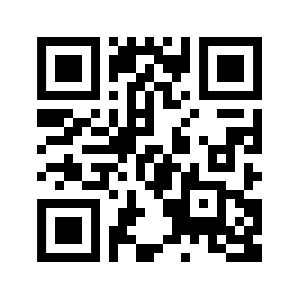
\includegraphics[scale=0.5]{tcc/figures/exemplo-qrcode.png}
    \caption{Exemplo de um QRCode}
    \legend{Fonte: O Autor.}
    \label{fig-exemplo-qrcode}
\end{figure}

\section{O que é CAPTCHA?}
\label{secao-captcha-definicao}

O CAPTCHA\cite{captchaWikipedia} é um acrônimo, em inglês, para "Completely Automated Public Turing Test to Tell Computers and Humans Apart", que pode ser traduzido como "Teste de Turing público completamente automatizado para distinção entre computadores e humanos", que nada mais é do que um desafio cognitivo para o impedimento de uso de ferramentas automáticas em sistemas. O uso de algumas dessas ferramentas podem fazer que em determinados casos, quando utilizados com abuso e/ou má-fé, levem a um consumo elevado dos recursos de alguns serviços, consequentemente, podem prejudicar a experiência de outros usuários desses mesmos serviços.

As versões mais simples do CAPTCHA consiste em uma imagem com uma frase (podendo ter sentido ou não) ou um conjunto de caracteres alfanuméricos\cite{captchaTecmundo}, e um campo de entrada de texto para que o usuário digitasse o conteúdo contido nessa imagem, caso o mesmo digitasse corretamente, o teste estaria concluído com êxito, fazendo com que a funcionalidade requisitada, protegida por esse teste, fosse liberada.

% FIXME: Ajustar a imagem
% FIXME: Adicionar referencia a imagem
\begin{figure}[h]
    \centering
    
\includegraphics[scale=0.5]{tcc/figures/captcha/captcha-frase.jpg}
    \caption{Exemplo de um CAPTCHA simples}
    \legend{Fonte: Wikipedia\cite{captchaWikipedia}}
    \label{fig-exemplo-captcha-simples}
\end{figure}

% FIXME: Ajustar a imagem
% FIXME: Adicionar referencia a imagem
\begin{figure}[h]
    \centering
    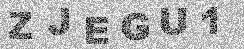
\includegraphics[scale=0.5]{tcc/figures/captcha/captcha-alfanumerico.png}
    \caption{Exemplo de um CAPTCHA simples com texto alfanumérico}
    \legend{Fonte: Wikipedia\cite{captchaWikipedia}}
    \label{fig-exemplo-captcha-alfanumerico}
\end{figure}

Esse tipo de teste pode ser burlado por algumas ferramentas automáticas uma vez que existe a possibilidade de efetuar a detecção de texto em uma imagem, tal técnica é conhecida como OCR ("Optical Character Recognition", em português: "Reconhecedor Ótico de Caracteres").\cite{captchaExame}

Atualmente, existem versões mais modernas desses testes que exigem que o usuário clique em uma imagem aleatória, o que dificulta o trabalho de ferramentas fraudadoras desses testes.\cite{captchaExame}

% FIXME: Ajustar a imagem
% FIXME: Adicionar referencia a imagem
\begin{figure}[h]
    \centering
    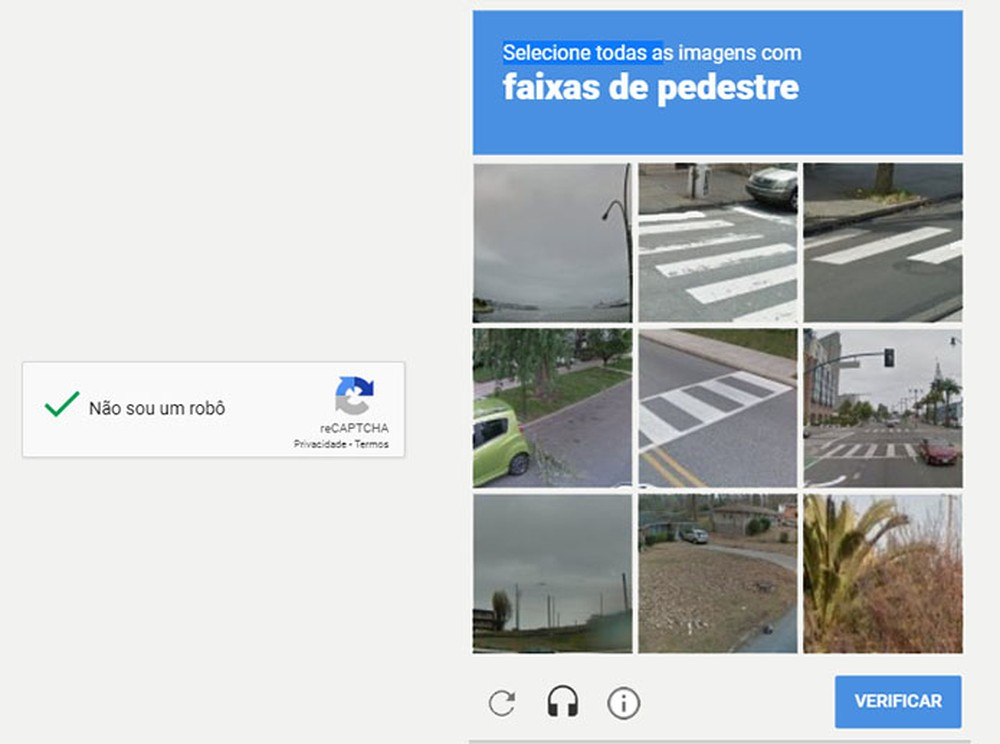
\includegraphics[scale=0.15]{tcc/figures/captcha/recaptcha-post-g1.jpg}
    \caption{Exemplo de um CAPTCHA moderno}
    \legend{Fonte: G1\cite{captchaG1}}
    \label{fig-exemplo-captcha-alfanumerico}
\end{figure}

\section{A Nota Fiscal de Consumidor Eletrônica}\label{secNfce}

A Nota Fiscal de Consumidor Eletrônica (NFC-e) visa ser uma alternativa eletrônica aos antigos cupons fiscais emitidos em papel. Tal documento segue um modelo nacional de emissão de documento fiscal com validade jurídica garantida pela assinatura digital do emissor.

Com a publicação do Decreto nº 44.785 em 12 de maio de 2014, a NFC-e foi instituída no Estado do Rio de Janeiro a partir do dia seguinte à publicação. Com isso, todos os estabelecimentos comerciais deveriam estar aptos ao uso da NFC-e até o dia 31 de dezembro de 2017.\cite{nfceDefinicao}

% FIXME: Ajustar a imagem
% FIXME: Adicionar referencia a imagem
\begin{figure}[h]
    \centering
    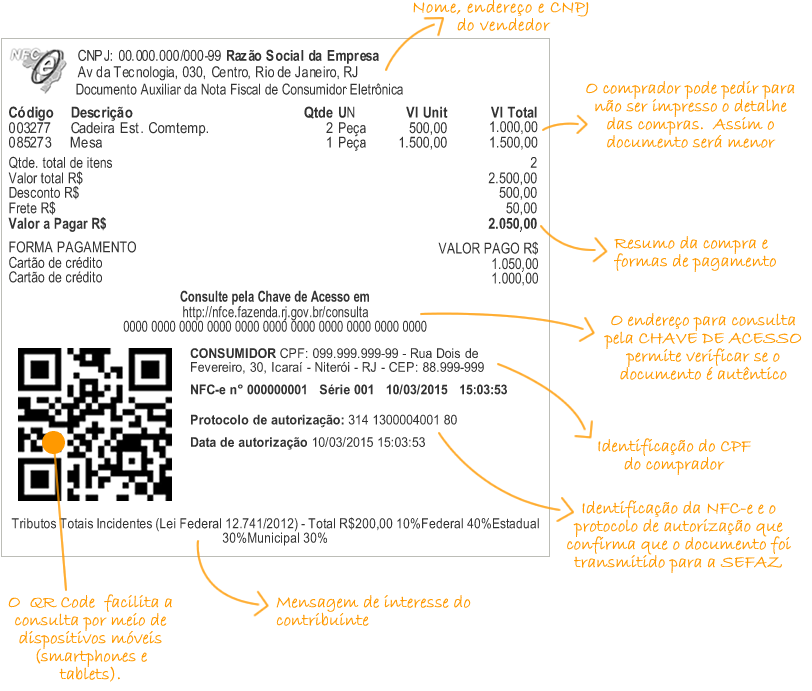
\includegraphics[scale=0.5]{modelo_nota_fiscal}
    \caption{Exemplo de uma NFC-e}
    \legend{Fonte: Secretaria de Fazenda - RJ}
    \label{modeloNfce}
\end{figure}

Na \autoref{modeloNfce} é possível observar um exemplo de uma NFC-e, com isso, pode se observar a descrição, a quantidade e o preço unitário de cada produto comprado. Além disso, ainda consta a informação do estabelecimento onde a compra foi efetuada como o endereço, o CNPJ e nome do estabelecimento.

Ainda, nesse documento consta uma chave de acesso que é composta por 44 dígitos e um QRCode. De posse desses dados, é possível acessar a versão online da respectiva nota, na qual contém as mesmas informações a respeito da compra assim como existe em sua versão física.

% TODO: Adicionar print imagem nota online?

A verificação de autenticidade pode ser efetuada através de um site disponibilizado e mantido por cada Secretaria de Fazenda dos estados que constituem a União. Sendo assim, não é possível verificar a autenticidade de uma NFC-e emitida no estado de São Paulo na plataforma disponibilizada pela Secretaria de Fazenda do Estado do Rio de Janeiro.

\section{Aplicativos semelhantes}

Existem aplicativos disponíveis para download nas lojas das plataformas IOS e Android com uma proposta semelhante ao trabalho desenvolvido. Como exemplo, pode ser citado o \textbf{Menor Preço}\cite{menorPrecoApp}, que é desenvolvido e mantido pelo Governo do Estado do Paraná. Através desse aplicativo, é possível consultar os preços de qualquer estabelecimento dos estados do Paraná, Espirito Santo e Pernambuco, no entanto, as informações das compras são obtidas diretamente das secretarias de fazenda de cada estado, não sendo necessário o usuário efetuar o cadastro de suas notas. Existem ainda outros aplicativos com esse mesmo funcionamento para outros locais como o \textbf{Melhor Preço Amazonas}\cite{melhorPrecoAmazonasApp} e o \textbf{Meus Preços (São Paulo)}\cite{meusPrecosApp}.

Outro aplicativo que possui abrangência nacional e que o funcionamento se assemelha ao desenvolvido nesse projeto é o \textbf{Pinngo}\cite{pinngoApp}, onde sua base de dados é feita através da contribuição dos usuários.
	\chapter{Desenvolvimento}

\section{A Nota Fiscal de Consumidor Eletrônica}

%% FIXME: ReferÊncia http://nfce.encat.org/institucional/o-que-e-nfc-e/
A Nota Fiscal de Consumidor Eletrônica (NFC-e) visa ser uma alternativa eletrônica aos antigos cupons fiscais emitidos em papel. Tal documento segue um modelo nacional de emissão de documento fiscal com validade jurídica garantida pela assinatura digital do emissor.

Com a publicação do Decreto nº 44.785 em 12 de maio de 2014, a NFC-e foi instituída no Estado do Rio de Janeiro a partir do dia seguinte à publicação. Com isso, todos os estabelecimentos comerciais deveriam estar aptos ao uso da NFC-e até o dia 31 de dezembro de 2017.

% FIXME: Ajustar a imagem
% FIXME: Adicionar referencia a imagem
\begin{figure}[h]
    \centering
    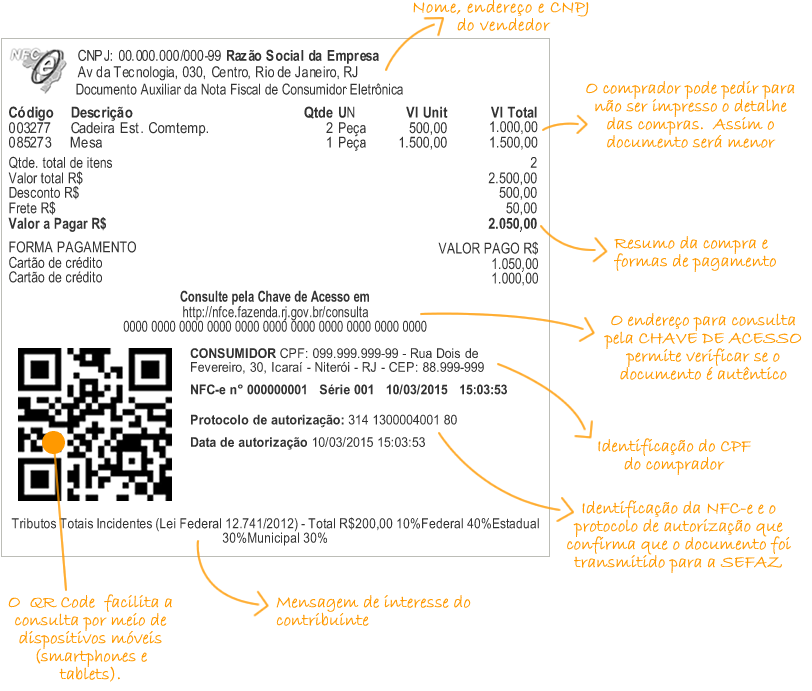
\includegraphics[scale=0.5]{modelo_nota_fiscal}
    \caption{Exemplo de uma NFC-e}
    \label{modeloNfce}
\end{figure}

Na figura \ref{modeloNfce} é possível observar um exemplo de uma NFC-e, com isso, pode se observar a descrição, a quantidade e o preço unitário de cada produto comprado. Além disso, ainda consta a informação do estabelecimento onde a compra foi efetuada como o endereço, o CNPJ e nome do estabelecimento.

Ainda, nesse documento consta uma chave de acesso que é composta por 44 dígitos e um QR Code, de posse desses dados é possível acessar a versão online da respectiva nota, no qual contém as mesmas informações a respeito da compra assim como existe em sua versão física.

% TODO: Adicionar print imagem nota online?

A verificação de autenticidade pode ser efetuada através de um site disponibilizado e mantido por cada Secretaria de Fazenda dos estados que constituem a União. Sendo assim, não é possível verificar a autenticidade de uma NFC-e emitida no estado de São Paulo na plataforma disponibilizada pelo Secretaria de Fazenda do Estado do Rio de Janeiro.

Essa peculiaridade, faz com que a versão desenvolvida descrita nesse projeto, tenha suporte a somente notas emitidas no estado Fluminense. Todavia, a adição do suporte a outros estados é facilitada, pois a inclusão já foi prevista durante o desenvolvimento.

\section{Obtenção das informações}
\label{obtencaoInformacoes}

O usuário pode acessar a versão da online da nota fiscal através de duas formas: a partir de um site específico junto de uma chave de acesso ou pelo site contido no QRCode. Após o usuário solicitar a adição de uma nota fiscal no aplicativo é feita uma simulação de uma dessas formas de acesso resultando em uma requisição ao site da Secretaria de Fazenda.

Independente de que forma foi efetuado o acesso, após o término da solicitação, o usuário é redirecionado para uma página que contém a versão online da nota fiscal. O conteúdo dessa página é analisado e armazenado. A técnica utilizada para a análise desse conteúdo é o Web Scraping.

\subsection{Simulação da solicitação}

Conforme dito anteriormente, independente da forma de acesso à nota, o mesmo conteúdo poderá ser obtido, porém os processos de reprodução dessas formas possuem algumas diferenças entre si.

A solicitação através da chave de acesso é feita de forma a simular o acesso do usuário ao site original, isto é feito com o auxílio da biblioteca Puppeteer para o Node.js é possível reproduzir a navegação em um navegador. Desta forma, o site disponibilizado para consulta das notas é acessado com o auxílio dessa ferramenta, no entanto, para obter o conteúdo da nota é necessário que um código de verificação (código Captcha) também seja inserido para que se possa comprovar que a solicitação está sendo feito por um humano e não por ferramentar automatizadas, logo, esse código é repassado para o usuário do aplicativo para que a requisição possa ser validada.

% FIXME: Melhorar esse trecho.

Caso a nota fiscal já esteja disponível e o código de verificação esteja correto, o conteúdo será disponibilizado, caso contrário, o usuário será notificado que houve um erro durante o cadastro da NFC-e na aplicação.

Já para reprodução com o QRCode, é possível obter o conteúdo diretamente sem a necessidade de inserção de código de verificação, todavia, ainda é necessária a simulação da navegação com o Puppeteer.

Assim como no forma anterior, caso a NFC-e não seja encontrada no sistema da SEFAZ, o usuário também será notificado que a mesma não encontra-se disponível.

Vale destacar que para a adição da NFC-e com o QRCode, é necessário o usuário possua um smartphone com câmera.

Caso qualquer error não previsto durante o processamento da requisição ocorra ou o sistema da SEFAZ esteja inoperante, o usuário também será notificado sobre a impossibilidade da adição com uma mensagem de erro genérica. Tal situação poderá ocorrer independente de que forma foi feita a solicitação.

\subsection{Análise dos dados}

A análise dos dados é feita com o auxílio da ferramenta Cheerio, que é um módulo baseado no jQuery, um framework bastante popular do JavaScript, para utilização com o Node.js. Com o conteúdo da página, é possível obter cada informação individualmente, logo é possível quais produtos foram comprados como o preço unitário e quantidade comprada de cada. Além disso, também é possível armazenar os dados do local da compra como o nome do estabelecimento e o seu endereço. Por fim, dados gerais da compra também podem ser recuperados como a data e a hora em que foi realizada.

A recuperação da informação da página pois o conteúdo é construído com a linguagem HTML e através dos elementos que compõe a página, é possível identificá-los e efetuar a separação da informação.

\section{Armazenamento das informações}
\label{armazenamentoInfo}

% TODO: Modelagem dos dados
% https://medium.com/@gpanassol/como-posso-fazer-modelagem-de-dados-em-mongodb-ea61268ee10b
% https://felipetoscano.com.br/modelando-dados-no-mongodb/
% file:///home/vitor/%C3%81rea%20de%20Trabalho/[NoSQL%20e%20MongoDB%20Users]%20Modelagem%20de%20Dados%20para%20BD%20Orientado%20a%20Documentos.pdf
% https://www.univates.br/bdu/bitstream/10737/1674/1/2017MarcelKober.PDF
% https://www.monografias.ufop.br/bitstream/35400000/1963/6/MONOGRAFIA_An%C3%A1liseProjetosBanco.pdf
Com os dados provenientes da NFC-e já processados, ou seja, analisados e separados, esse conteúdo resultante é armazenado em um banco de dados para que a informação seja disponibilizada posteriormente para consultas a partir da aplicação.

Esse conteúdo é armazendao em um banco de dados e o tipo utilizado pela aplicação é o MongoDB, que é um banco de dados não-relacional com os dados sendo armazenados em formato de documento. Como a aplicação está sendo feita em JavaScript, foi optado em utilizar essa banco devido a conveniência resultante do uso junto ao Json.

Além disso, esse tipo de banco é altamente escalável, isto é, caso seja necessário mais espaço para o armazenamento dos dados, o conteúdo pode ser distribuído em diversas máquinas sem afetar o desempenho geral da aplicação.

\subsection{Justificativa do uso de Armazenamento Remoto e Dados Compartilhados}

Os dados provenientes do processamento das notas fiscais poderiam ser armazenados nos celulares dos usuários do aplicativo, o que resultaria no consumo de espaço de armazenamento que é também compartilhado com outros aplicativo e o sistema operacional do aparelho móvel. Embora seja uma alternativa viável para o cliente, e possivelmente rápida, uma vez que a recuperação não sofrerá latência de rede, a longo prazo talvez não seja considerada muito atrativa. A justificativa dessa afirmação é o fato de que para cada nota adicionada uma parcela do armazenamento é consumida, ademais, não existe uma rotina de limpeza dos dados mais antigos.

Apesar da implementação dessa rotina ser simples, restringiria uma possível melhoria ao produto, por exemplo, a disponibilização da série histórica de preços dos produtos a longo prazo.

Um outro ponto que pode ser destacado, é que com os dados concentrados no dispositivo de um indivíduo, os mesmos estão propensos a exclusão, que pode ser causada por diversas situações, por exemplo, a eliminação decorrente da remoção do aplicativo, a formatação do aparelho devido a restauração ao modo de fábrica ou até mesmo uma pane no aparelho em certos casos.

Após a observação dos pontos acima, a utilização de uma solução que envolva o armazenamento da informação em um meio externo torna-se viável, pois a segurança da informação é melhor garantida, uma vez que a cópia de segurança é garantida do lado do servidor desonerando o cliente dessa responsabilidade.

Uma vantagem garantida com ao preservar os dados dessa forma, é que uma base maior pode ser criada pois as notas de todos os usuários poderão estar guardadas em único local, o que acarreta em um compartilhamento de informação e a criação de uma base de dados colaborativa, aonde um usuário A adiciona sua NFC-e e os dados dos produtos estarão disponíveis para um usuário B, e caso esse último quisesse saber o custo de um produto comprado pelo usuário A, poderia consultá-lo por meio do aplicativo sem a necessidade de ir ao mercado utilizado pelo usuário A.

Vale destacar que, apesar da utilização de uma base compartilhada, não há como um usuário ter acesso ao valor gasto em uma compra de outro usuário, uma vez que as notas são adicionadas sem a necessidade de um cadastro e somente é possível obter a informação de produtos, e não de uma compra como um todo.

% TODO: Melhorar seção
\section{Disponibilização dos dados}

% Dependnecia de internet vs offilien
% Contraatacar com o processamento

% Processamento no proprio aparelho
% Usar do processador / bateria/internet de qualidade /

Os dados são disponibilizados com o auxílio do servidor principal da aplicação no qual possui uma conexão com o servidor em que se encontra o banco de dados.

% FIXME: Deve-se referenciar o Framework?
Através do Framework Express é possível criar de uma forma flexível uma API, que permite a comunicação com outras aplicações. Com isso, é disponibilizada uma URL que permite a consulta dos produtos salvos na base de dados.

A consulta é feita através do nome do produto, e esse nome pode estar acentuado corretamento, erroneamente ou até mesmo sem acentos, que os mesmos dados serão retornados.

Os dados retornados contém o nome do produto da forma que consta na nota fiscal, o nome do estabelecimento no qual a compra foi efetuada e a data e a hora da compra. Para cada produto compatível com a consulta, é retornado o último registro salvo para cada estabelecimento para que o usuário sempre possa ter o preço mais recente.

Vale ressaltar que é possível refinar a cidade em que a consulta deverá ser feita, assim como retornar os registros de todas as cidades disponíveis.

\subsection{Ausência de padronização nos nomes}

Um problema que pode ser observado a partir de uma simples consulta com o aplicativo é a ausência de padronização nos nomes dos produtos, haja vista que cada mercado cadastra em seu banco de dados as informações referentes aos produtos a seu bel-prazer. Como também, devido a espaço limitado nas notas fiscais impressas, faz com que ocorra uma abreviação nos produtos.

Uma alternativa aos nomes que poderia ser utilizada, poderia ser através do código de barras presente em cada produto, por outro lado, para aqueles produtos que são vendidos por peso, não há uma uniformidade no código desses produtos, ficando a critério de cada estabelecimento definir um código.

Visto esses problemas descritos, uma solução híbrida pode ser utilizada, isto é, dado um nome de um produto, com auxílio de serviços de terceiros, é possível recuperar o código de barras para o produto pesquisado, com isso, poderia efetuar a busca tanto pelo nome quanto pelo código de barras. Essa solução é sugerida como uma melhoria futura para a aplicação.

\section{Hospedagem}

Conforme descrito nas secções \ref{obtencaoInformacoes} e \ref{armazenamentoInfo}, um servidor torna-se necessário tanto para o processamento e disponibilização dos dados quanto para o armazenamento dos mesmos. Com isso um serviço de hospedagem faz-se necessário para ambos os casos.

\subsection{Backend}

Como todo processamento dos dados é feito em meio externo ao telefone móvel do usuário, logo, a utilização de um servidor é necessária e com isso será necessário a utilização de máquinas para poder executar o código desenvolvido para esse propósito. Um computador pessoal de baixo custo atende esse requisito, no entanto, a medida que o uso do aplicativo tornar-se mais frequente e a base de cliente for aumentando, uma máquina com mais recursos será imprescindível.

O uso de uma máquina física para esses propósitos é uma solução viável, no entanto, existem serviços que fornecem recursos de hospedagem a custo acessível e caso elegível, até mesmo, gratuito.

Uma das principais vantagens do uso de serviços de hospedagem é que o serviço não será interrompido caso haja queda de energia ou até mesmo ficar sem conexão com a internet.

Um dos serviços mais populares que oferecem tais recursos de hospedagem é o Heroku, que fornece desde uma máquina simples gratuita até serviços mais robustos focados para o uso de alto fluxo de dados como ocorre em grandes corporações.

Durante o desenvolvimento os primeiros meses de desenvolvimento, foi feito o uso da plano gratuito para testes, no entanto caso não houvesse nenhuma iteração com a API desenvolvida durante um período de 30 minutos, a mesma ficaria inativa. Diante desse fato, a solicitação de adição de notas tornava-se mais lenta pois além do tempo de processamento dos dados, o tempo de inicialização aumentava a latência em que a resposta era retornada ao usuário. Todavia, a iteração ainda poderia ser feita normalmente.

% TODO: Add ref https://education.github.com/pack
A empresa GitHub, que permite que desenvolvedores e empresas armazenem e divulguem seus códigos, possui um programa para estudantes que permite que os mesmos acessem e usufruem de recursos pagos sem gerar nenhum ônus. Esse programa é conhecido como GitHub Student Developer Pack que é feito em parceria com outras empresas do ramo da tecnologia.

O Heroku é um serviço que está incluso nessa parceria fornecendo uma máquina paga com muitos recursos sem nenhum custo ao estudante participante desse programa por um período limitante. Como o autor é elegível, o uso dessa máquina paga está sendo feito para os testes simulando o uso real de um servidor que pode ser utilizado em produção, isto é, recebendo altas cargas de requisições.

Outras empresas que poderiam ser utilizadas seriam a DigitalOcean, Locaweb, Hostgator e quaisquer outras com recursos semelhantes.

\subsection{Banco de Dados}

% TODO: Adicionar sugestões
% Acho que sim, voce pode mencionar os benefícios que voce teve por ser estudante, no momento do desenvolvimento do trabalho.
% E tambem mostrar alternativas para qunado nao é estudante.

\section{Desenvolvimento do aplicativo}\label{desenvApp}

O desenvolvimento do aplicativo é feito utilizando uma tecnologia de desenvolvimento multiplataforma com código nativo, para isso foi utilizado o React Native. Com isso, é possível desenvolver um único aplicativo e publicar para as duas plataformas mais populares, isto é, o IOS e o Android.

Com isso foi feito o desenvolvimento de único aplicativo que pode ser utilizado nas duas plataformas mencionadas acima. Sendo feito dessa forma, houve uma otimização no tempo de desenvolvimento.

% FIXME: Referenciar o ranking?
A justificativa para a escolha do uso do React Native, primeiramente é pelo fato de permitir um desenvolvimento multiplataforma com código nativo, em acréscimo, estava melhor colocado no ranking elaborado pelo StackOverflow, \textcolor{red}{\textbf{[presente na seção {TEMP} Devo referenciar o ranking?]}} quando comparado com seus concorrentes diretos. Além disso, caso futuramente seja disponibilizado as mesmas funcionalidades presentes no aplicativo para um website, isso poderá ser feito sem muitas complicações, sendo necessária poucas alterações.

\subsection{Expo}

%% FIXME:  Add ref https://docs.expo.io/versions/v36.0.0/; https://docs.expo.io/versions/latest/sdk/overview/
O Expo é um Framework e uma plataforma para aplicações de React. Com isso, acaba por ser um conjunto de ferramentas e serviços criadas em torno do React Native e das plataformas nativas que permite ao programador, desenvolver e distribuir sua aplicação entre os sistemas facilmente, a partir do mesmo código desenvolvido em JavaScript.

Além disso, o Expo proporciona uma abstração dos recursos de aparelhos móveis sem a necessidade de implementação de código nativo. Os recursos são tais como os contatos, a câmera, acesso ao GPS e dentre outros. Com isso, é possível recuperar a informação proveniente desses através do próprio código em JavaScript.

Com isso, foi optado em utilizar essa ferramenta de forma a acelerar o desenvolvimento do aplicativo. Como também é necessário o acesso a câmera para a leitura de QRCodes, tal ferramenta tornou-se indispensável, pois, por ser uma abstração de código nativo, é possível disponibilizar essa funcionalidade para ambas as plataformas sem complicações.

% Explicar a facilidade que o Expo proporciona
% Port para as aplicações

\subsection{Estilização}

De forma a acelerar o tempo de desenvolvimento do aplicativo, algumas ferramentas foram utilizadas para a estilização do aplicativo. Tais ferramentas são um conjunto de componentes prontos, isto é, já estilizados, bastando somente efetuar a adaptação para o projeto como o posicionamento e o tamanho.

Desses recursos, foram utilizados dois pacotes de estilos, o NativeBase e o React Native Paper. Ambos, fornecem estilos semelhantes aos nativos disponíveis em cada plataforma.

% NativeBase
% Native Paper

% Falar aqui dos templates usados com o React Native
% Vantagem de manter o estilo nativo para o Android e o IOS
	\chapter{Resultados}

 Neste capítulo será apresentado o aplicativo desenvolvido e suas interfaces com o usuário onde terá a explicação de cada recurso disponível assim como efetuar sua utilização. Ainda, serão apresentadas algumas limitações existentes para essa versão da aplicação como também das tecnologias utilizadas.
 
\section{O aplicativo desenvolvido}
\label{sec-app-desenvolvido}

Conforme apresentado na seção \ref{desenvApp}, o aplicativo foi desenvolvido utilizando o React Native e fazendo o usufruto de alguns pacotes de estilização. O aplicativo é funcional, ou seja, é possível efetuar a instalação do mesmo em um smartphone e utilizar todos os seus recursos, no entanto, o mesmo não se encontra disponível para download através das lojas de aplicativos AppStore e PlayStore, respectivamente dos sistemas iOS e Android.

Embora não seja possível ainda instalar essa aplicação através das lojas oficiais das plataformas, para o sistema Android é factível efetuar a instalação de aplicativos por outros meios, através do download do arquivo referente aos mesmos. Tal procedimento necessita de algumas alterações nas configurações padrões do aparelho para que possa permitir a instalação de outras fontes. Caso não se tenha confiança na procedência da aplicação baixada, não é recomendado o prosseguimento da instalação.

\newpage
\subsection{Apresentação do aplicativo}

% FIXME: Ajustar a imagem
% FIXME: Adicionar referencia a imagem
\begin{figure}[h]
    \centering
    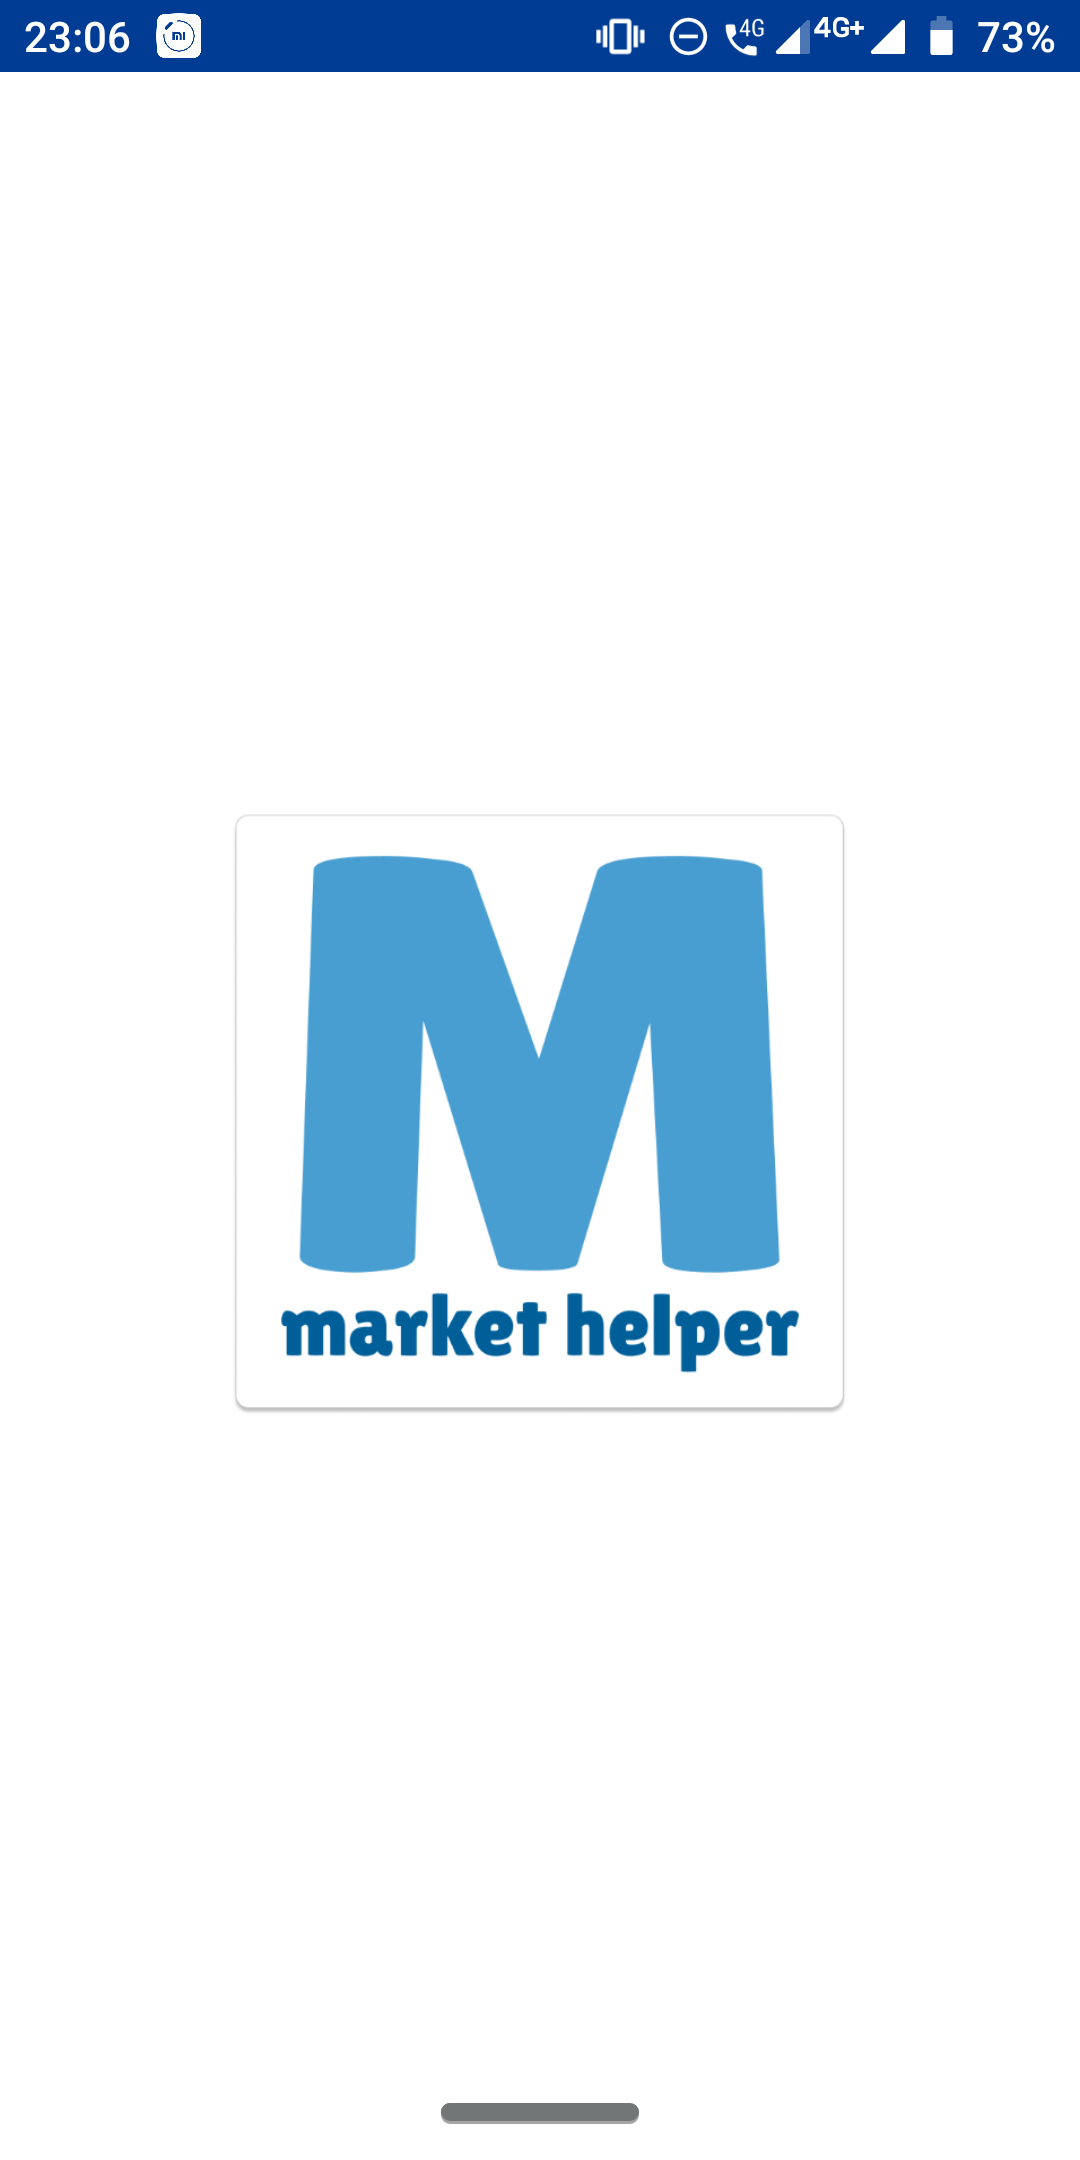
\includegraphics[scale=0.15]{tcc/figures/app/app_loading.png}
    \caption{Tela de carregamento inicial}
    \label{appLoadingFig}
\end{figure}

A figura \ref{appLoadingFig} representa a primeira tela que o usuário obtém ao efetuar a abertura da aplicação, além disso, essa tela é mostrada para que os recursos mínimos necessários ao aplicativo possam ser carregados em segundo plano. Com isso, sempre que o aplicativo for inicializado mostrará essa tela. Caso o usuário saia e vá para outro aplicativo, essa tela não será mostrada pois os recursos ainda estão em memória, mas caso o usuário encerre a aplicação, na próxima vez que houver a abertura, será necessário novamente efetuar o carregamento, logo, a tela de carregamento inicial será exibida outra vez.

% FIXME: Ajustar a imagem
% FIXME: Adicionar referencia a imagem
\begin{figure}[h]
    \centering
    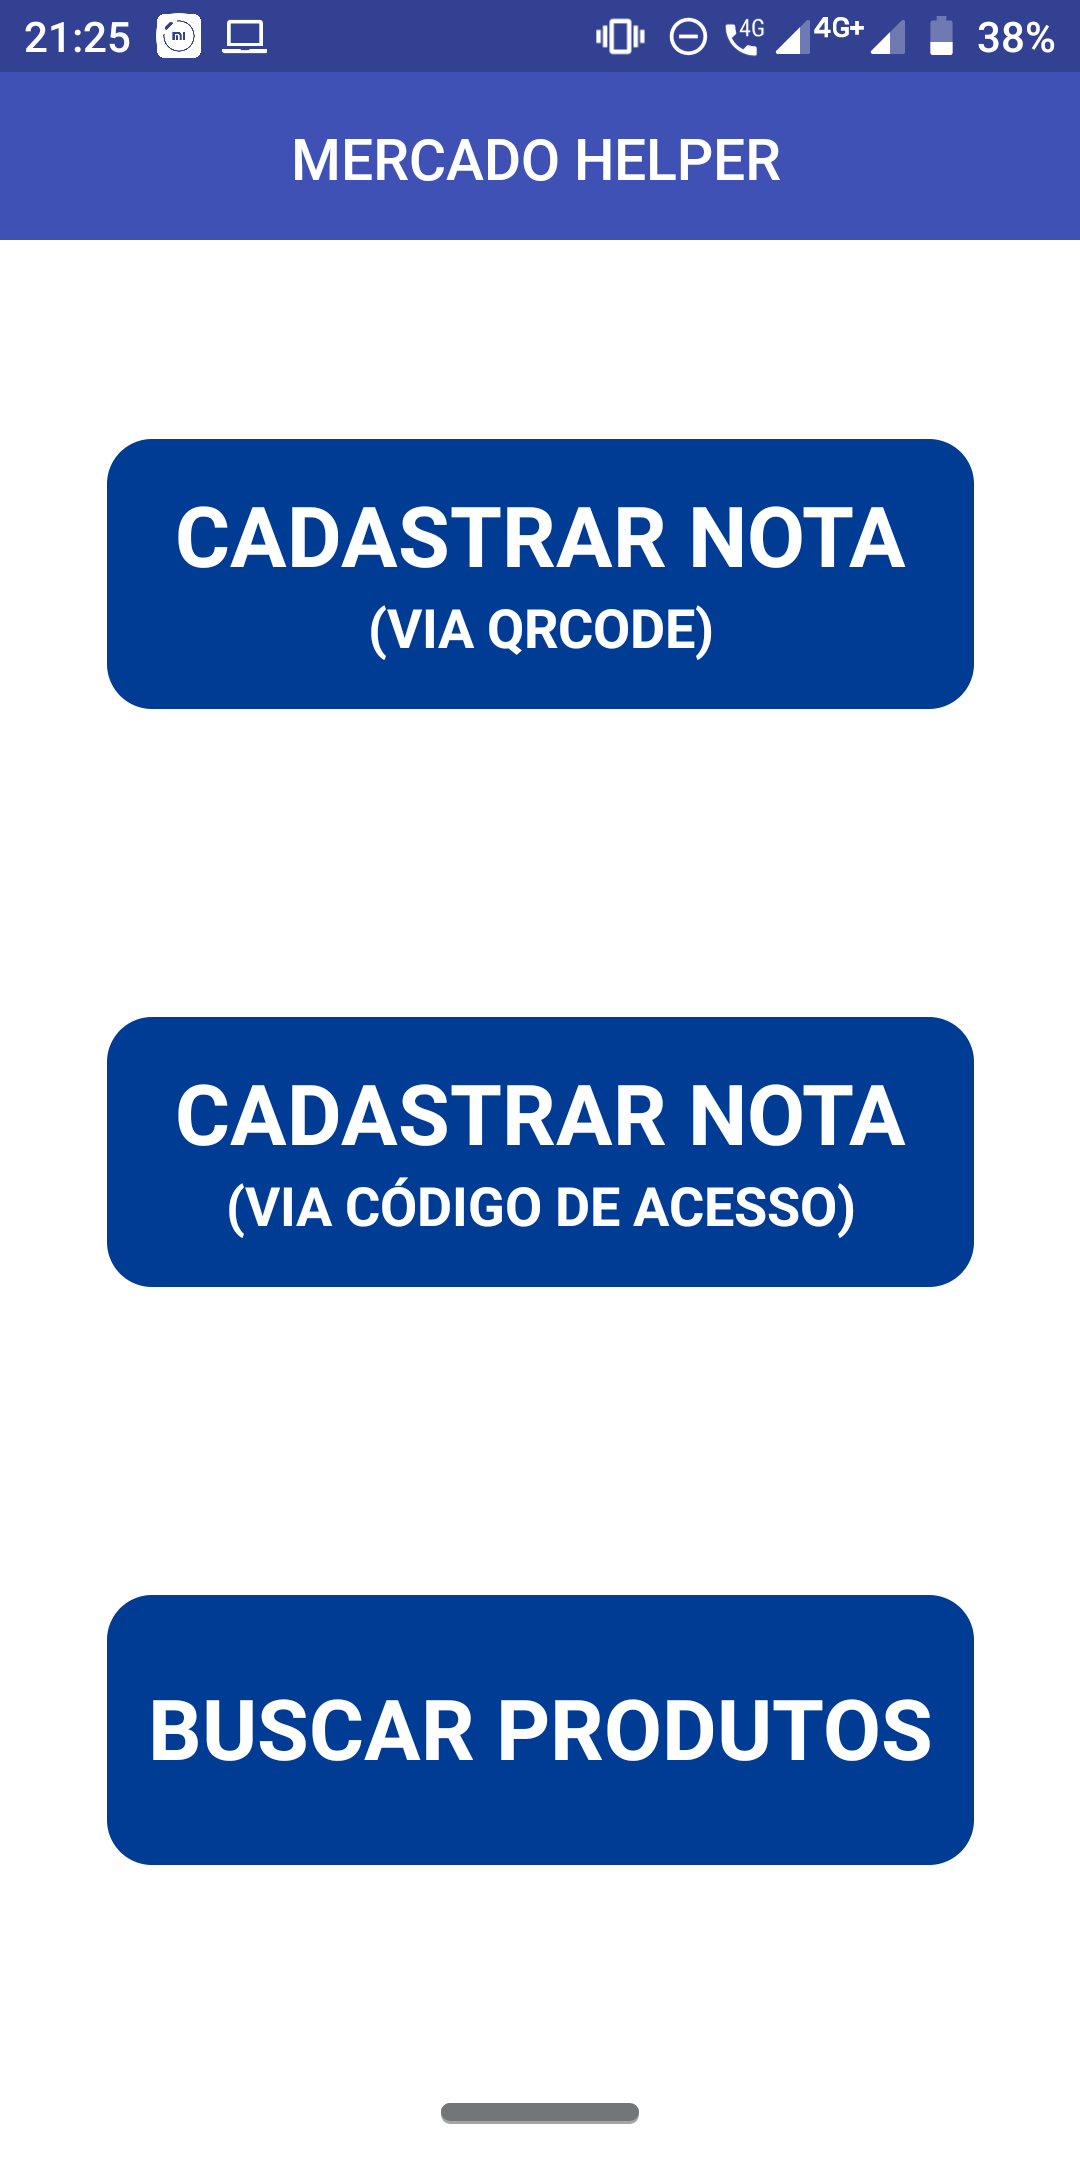
\includegraphics[scale=0.15]{tcc/figures/app/app_home.png}
    \caption{Tela principal}
    \label{appHomeFig}
\end{figure}

\newpage
Após o carregamento desses recursos, o usuário é automaticamente redirecionado para a tela principal do aplicativo, que é demonstrada através da figura \ref{appHomeFig}. A partir dessa tela, é possível efetuar a adição das notas fiscais como a busca por produto através dos atalhos.

No primeiro botão, é possível efetuar a adição da NFC-e através do QRCode presente na mesma. Para tal funcionalidade, é necessário que o dispositivo possua uma câmera e que o usuário conceda permissão para uso da mesma.

No segundo botão, o usuário poderá efetuar a adição através do código de acesso e no último botão, o mesmo poderá consultar a base de dados para obter as informações referentes aos produtos.

\subsection{Adição das notas fiscais}

O usuário poderá efetuar a adição das notas através de duas formas, a primeira que é através do QRCode presente nas versões impressas das mesmas bem como através do código de acesso também disponível na versão física da nota.

Dependendo da forma de adição desejada pelo usuário, o mesmo será redirecionado para outras telas que serão apresentadas logo abaixo.

O meio mais rápido de adicionar é aquele que utiliza o QRCode, pois basta apontar a câmera do smartphone para o código que a leitura do mesmo será feita instantaneamente.

Caso ocorra problemas na leitura desse código, o usuário poderá tentar adicionar através do código de acesso. Esse meio é um pouco mais lento, pois além de inserir esse código de 44 dígitos, será necessário adicionar um código de verificação da solicitação, isto é, o CAPTCHA.

\subsubsection{Através do QRCode}

% FIXME: Ajustar a imagem
% FIXME: Adicionar referencia a imagem
\begin{figure}[h]
    \centering
    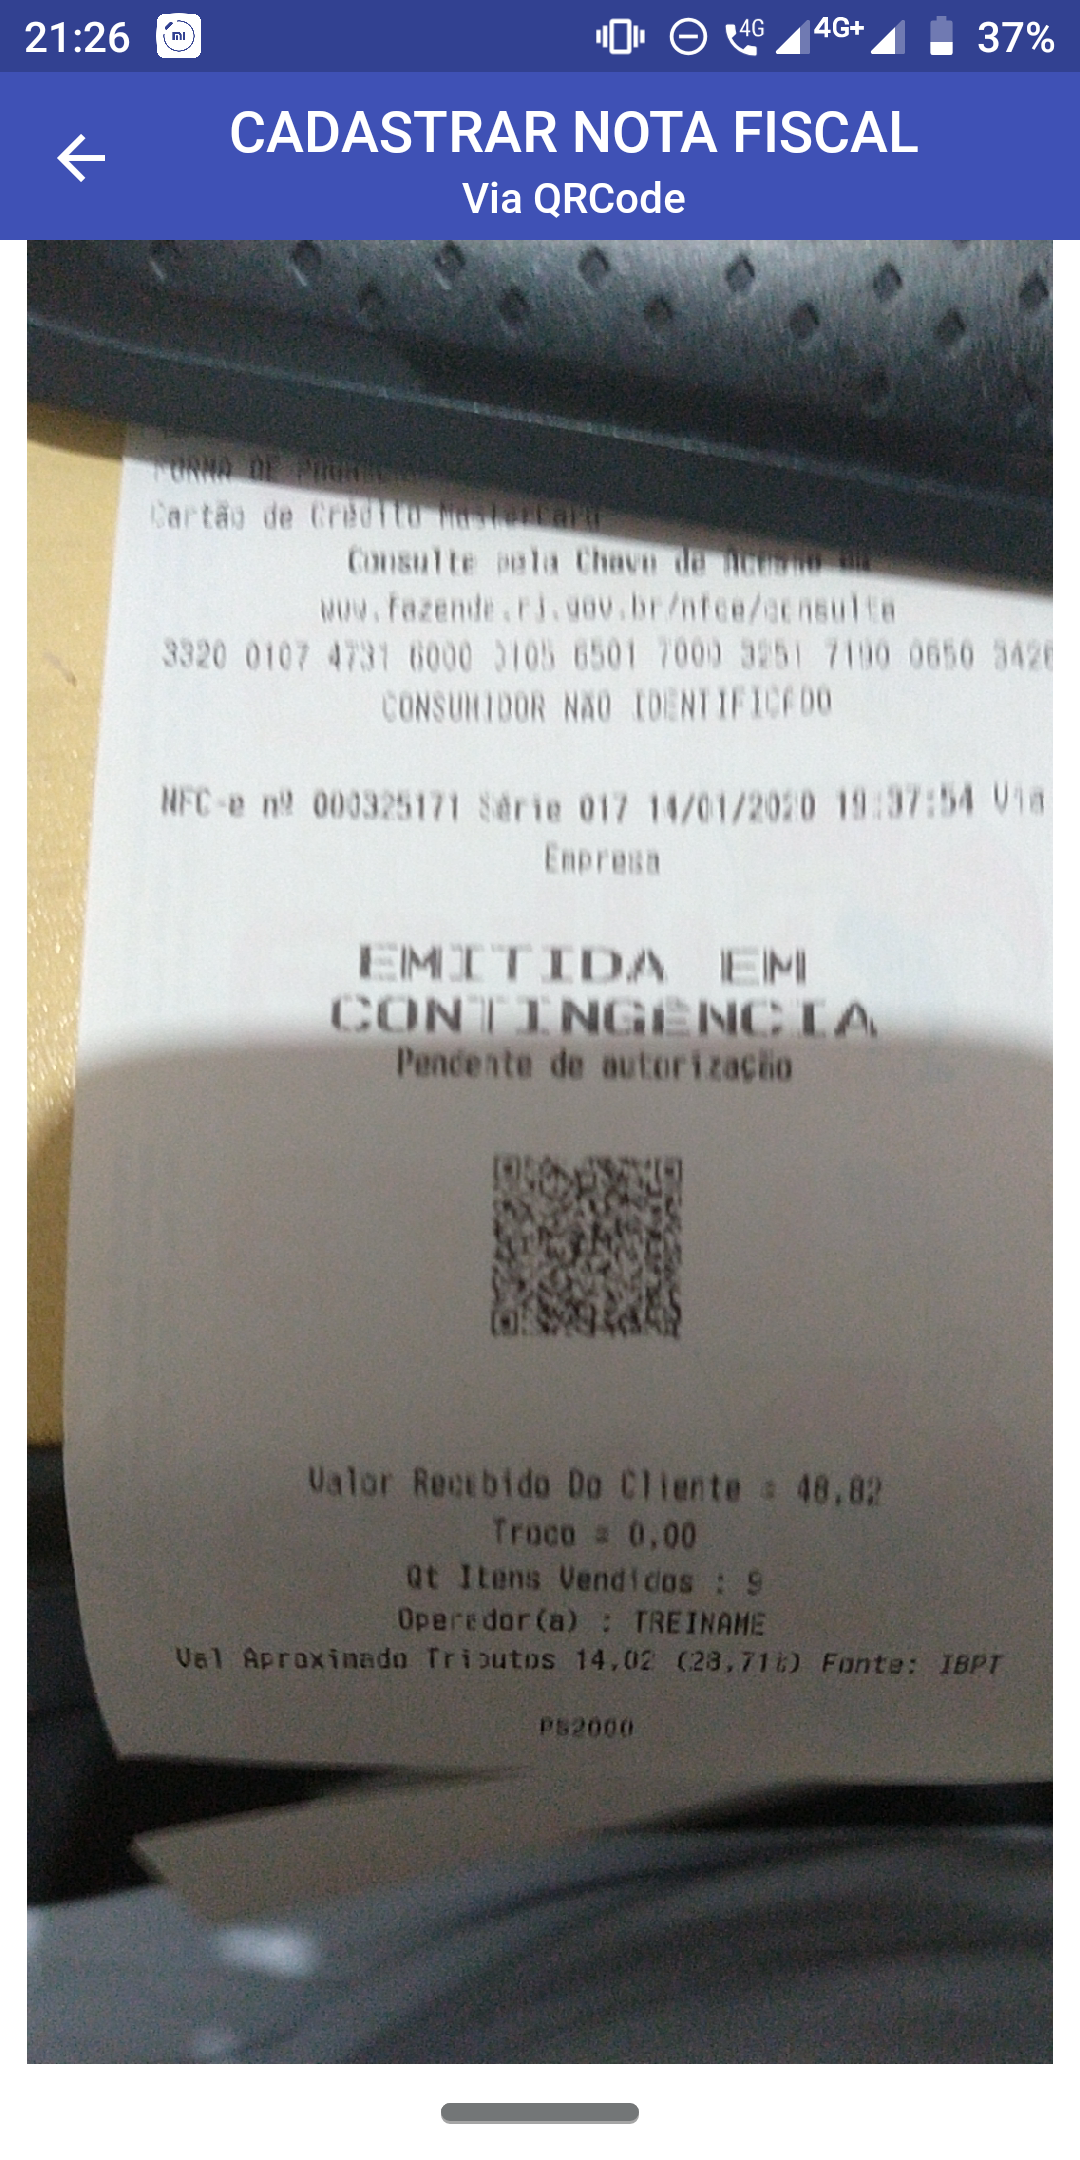
\includegraphics[scale=0.15]{tcc/figures/app/app_codigo_qrcode_solicitacao.png}
    \caption{Exemplo de adição de uma NFC-e real via uso do QRCode}
    \label{appQRCodeSolicitacaoFig}
\end{figure}

Um caso real de adição de uma nota fiscal é representando pela captura da tela do aplicativo no qual é demonstrado pela figura \ref{appQRCodeSolicitacaoFig}. Caso seja feita a detecção do QRCode, o conteúdo contido nesse código será processado e uma solicitação de adição será feita ao servidor.

A latência gerada durante esse período de processamento, faz com seja necessário o uso de uma tela de carregamento. Com isso, é mostrado para o usuário uma barra de progresso que indica que a sua solicitação está sendo processada e o aplicativo continua executando normalmente.

% FIXME: Ajustar a imagem
% FIXME: Adicionar referencia a imagem
\begin{figure}[h]
    \centering
    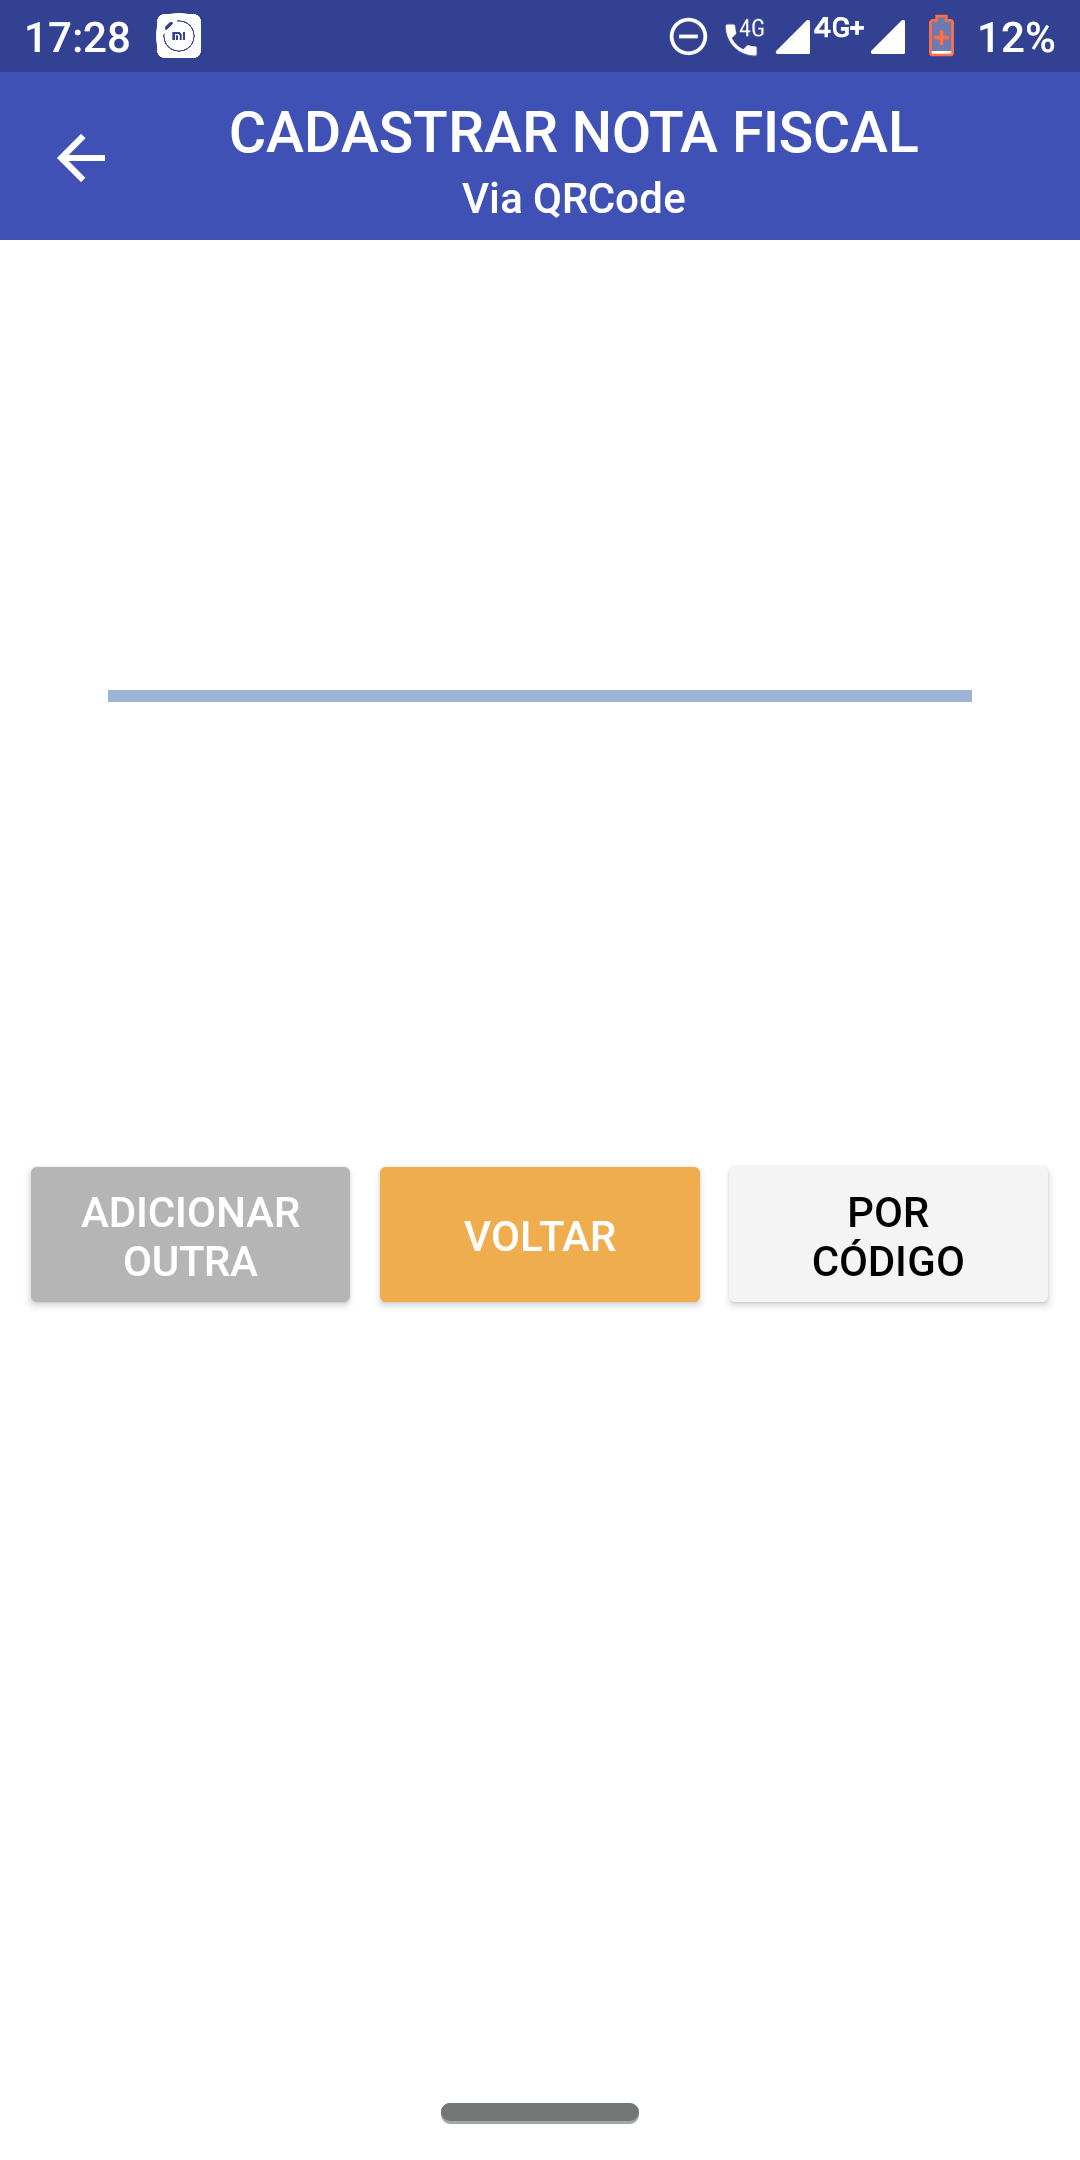
\includegraphics[scale=0.15]{tcc/figures/app/app_codigo_qrcode_loading.png}
    \caption{Tela de cadastro via QRCode após solicitação}
    \label{appQRCodeSolicitacaoFig}
\end{figure}

\newpage
Após o processamento ter terminado, podendo ter sido com sucesso ou não, será enviado para o aplicativo uma resposta contendo o status da solicitação de adição realizada.

Se o código tiver sido lido corretamente e se não houver nenhuma problema durante a solicitação da nota ao site da SEFAZ assim como também no processamento da nota, será mostrado uma mensagem de sucesso conforme pode ser observado na figura abaixo.

% FIXME: Ajustar a imagem
% FIXME: Adicionar referencia a imagem
\begin{figure}[h]
    \centering
    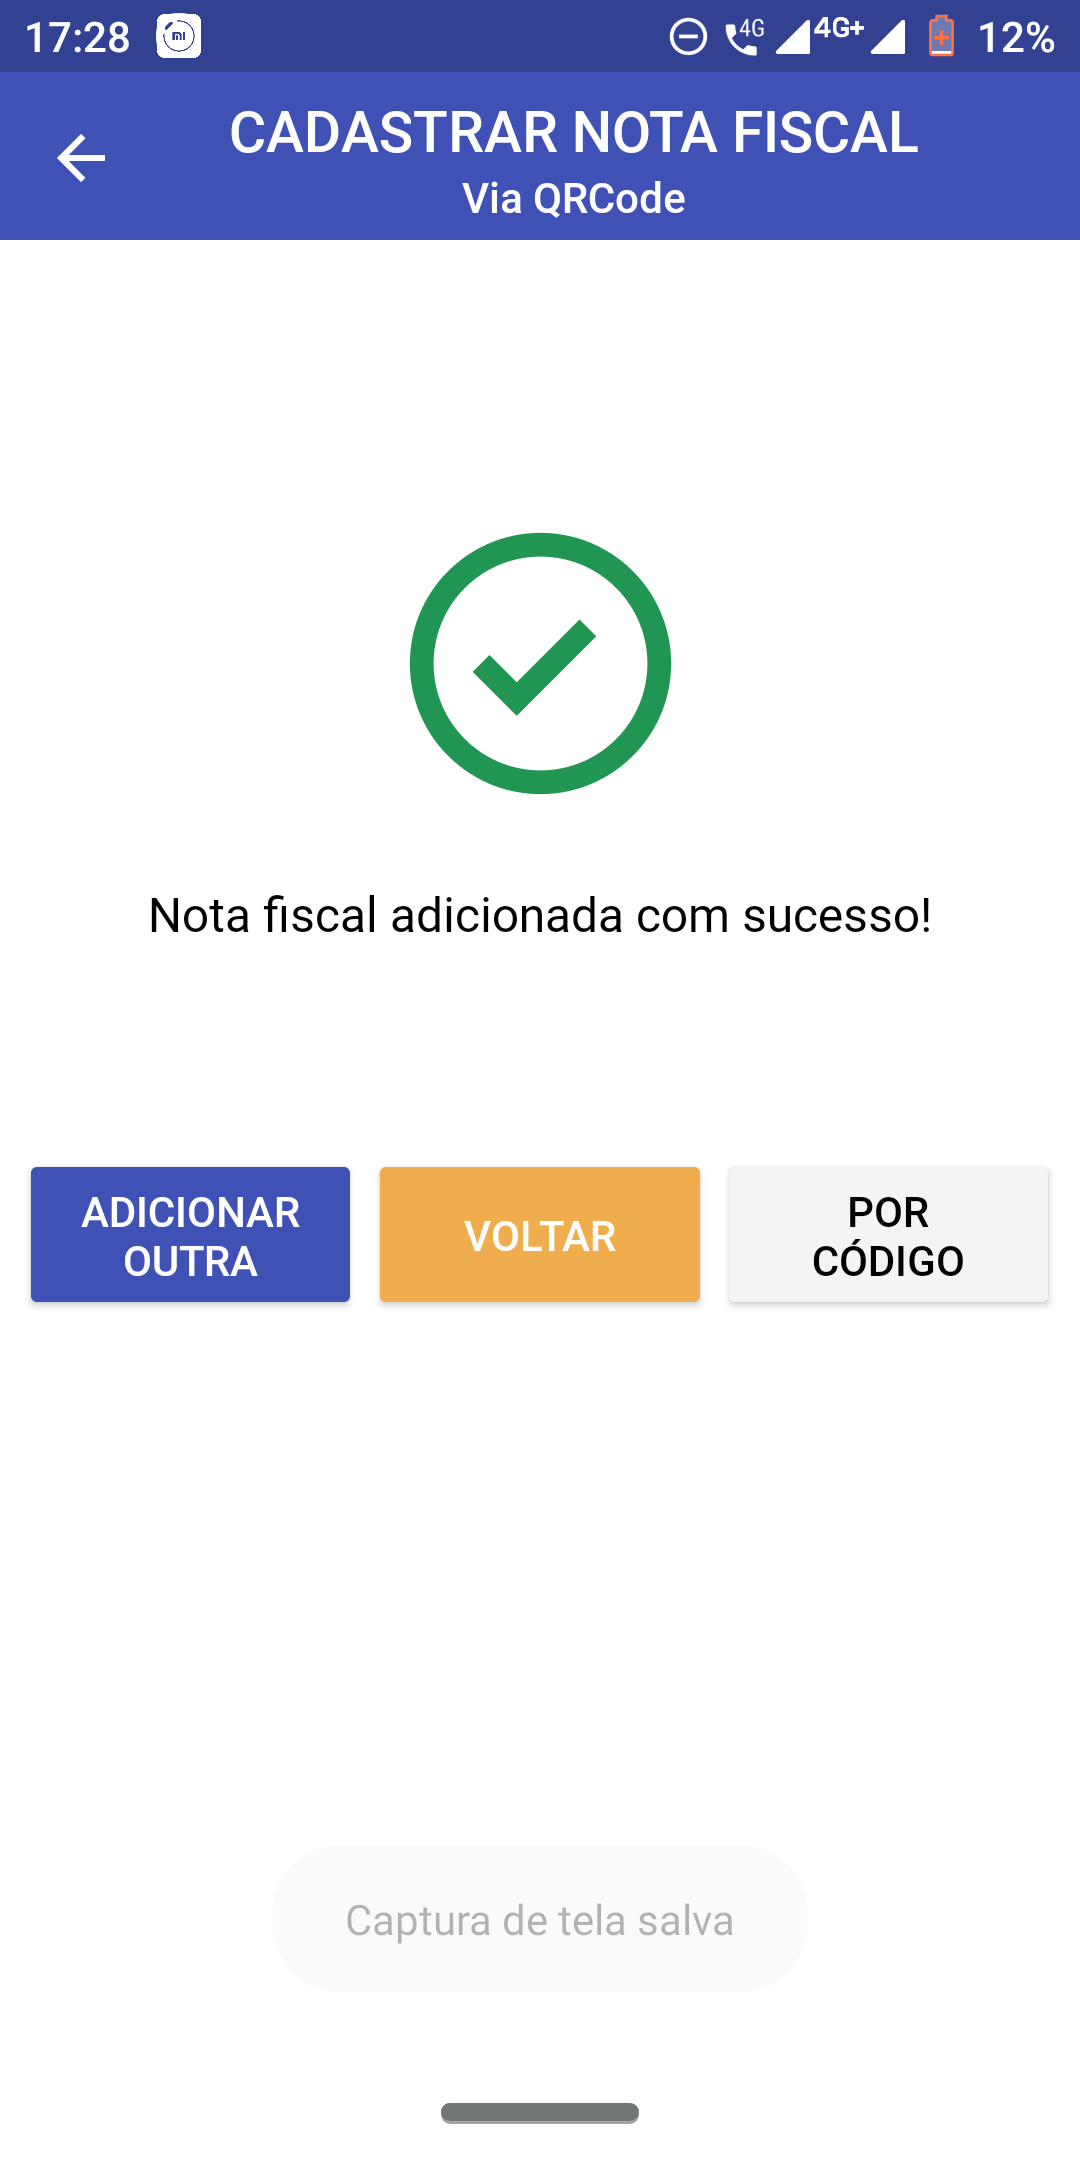
\includegraphics[scale=0.15]{tcc/figures/app/app_codigo_qrcode_sucesso.png}
    \caption{Tela de cadastro efetuado com sucesso}
    \label{appQRCodeSucessoFig}
\end{figure}

\newpage
Todavia, durante o processo de adição, pode ser que a nota ainda não esteja disponível no sistema da SEFAZ, com isso, é feito um tratamento de forma a detectar essa caso, com isso, o usuário será informado que a sua solicitação não foi concluída devido a indisponibilidade em sua versão digital. A figura \ref{appQRCodeNaoDisponivelFig} representa esse caso.

% FIXME: Ajustar a imagem
% FIXME: Trocar por img equivalente do QRCODE
% FIXME: Adicionar referencia a imagem
\begin{figure}[h]
    \centering
    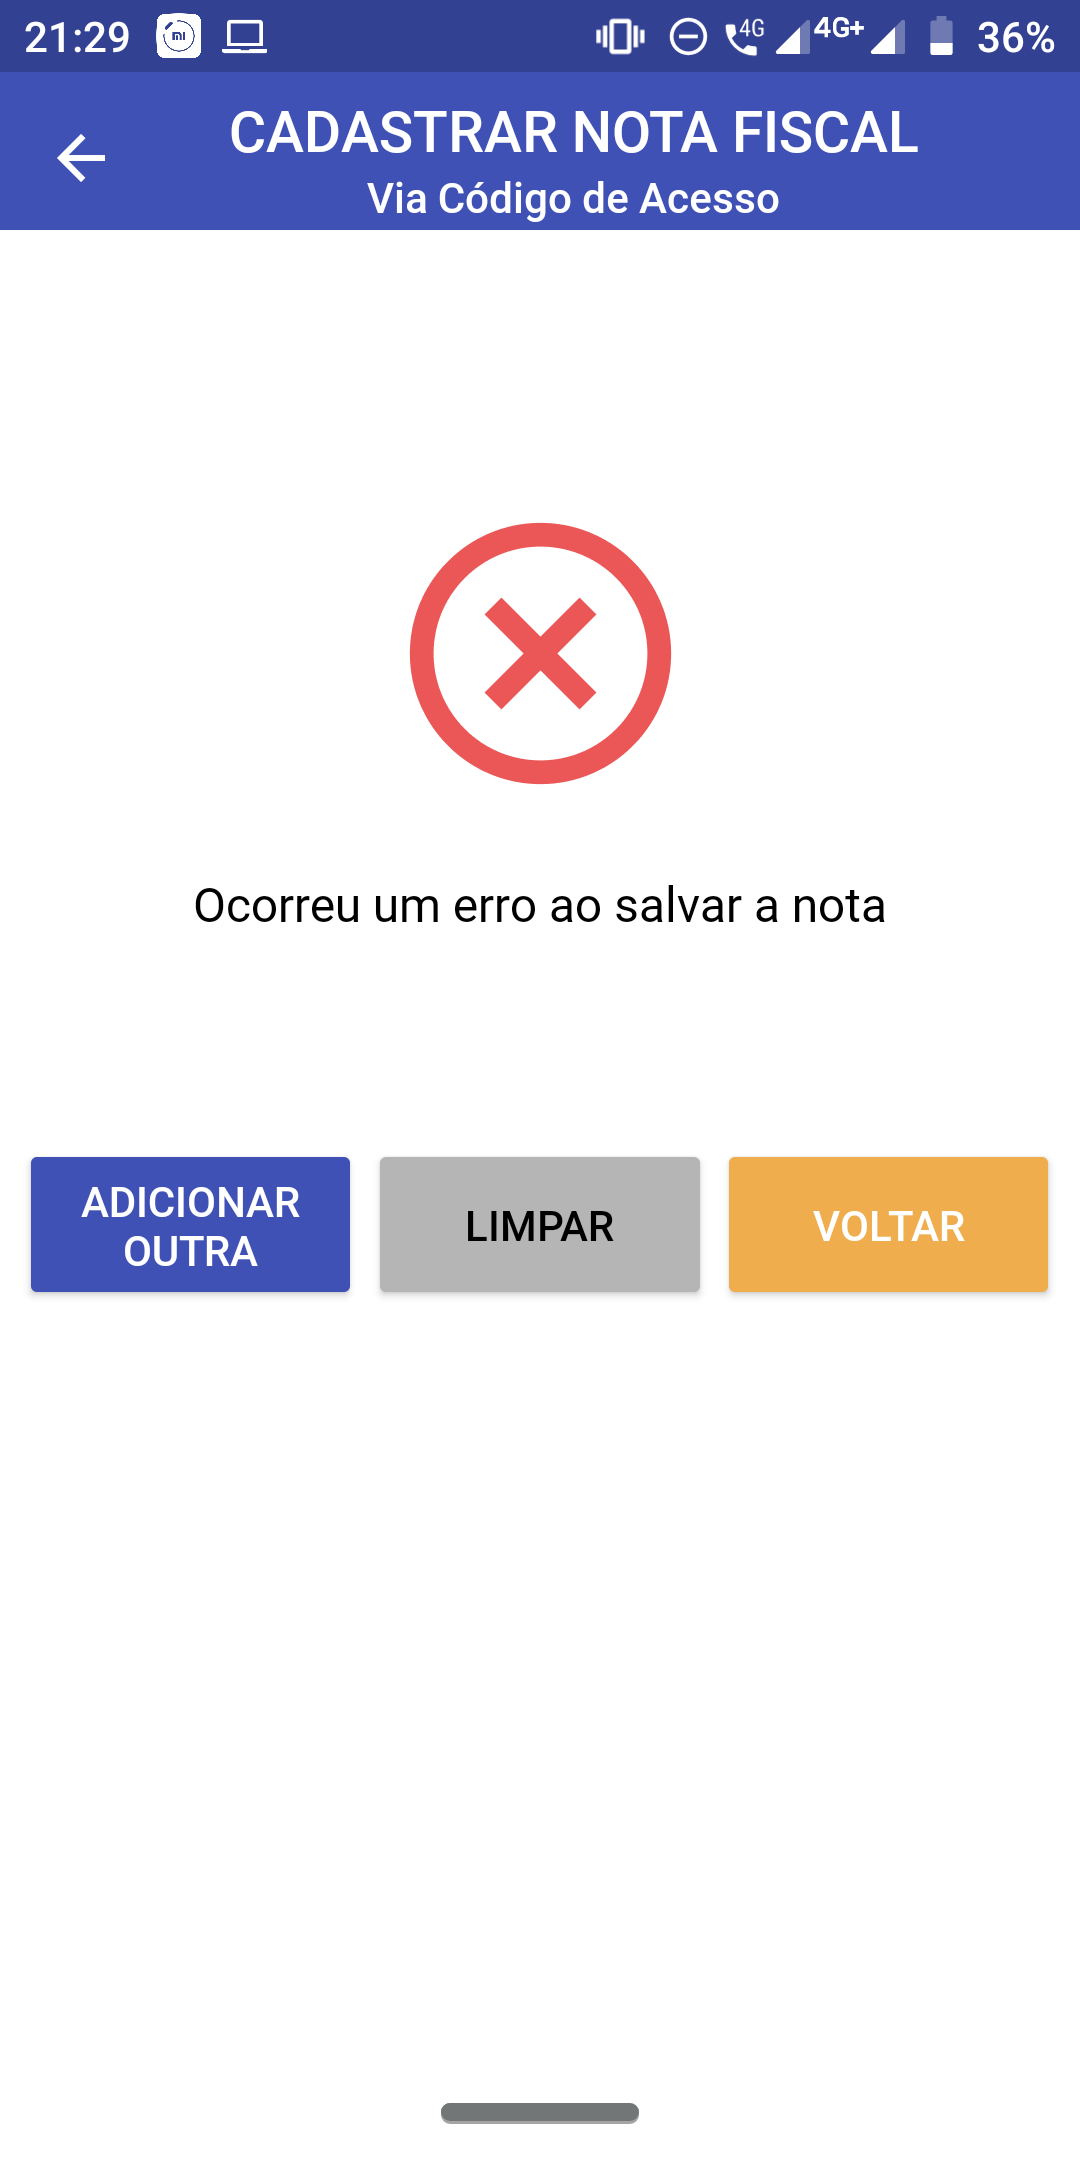
\includegraphics[scale=0.15]{tcc/figures/app/app_codigo_acesso_nao_disponivel.png}
    \caption{Tela de nota não disponível}
    \label{appQRCodeNaoDisponivelFig}
\end{figure}

\newpage
Uma outra situação que poderá ocorrer, é caso o usuário tente adicionar uma nota que já foi adicionada previamente. A solicitação ao sistema da SEFAZ será feita normalmente até a obtenção do código de acesso da NFC-e, que é um código único. Após a aquisição desse código, é feita uma pesquisa no banco de dados de forma a verificar a existência dessa nota nos registros. Caso a nota seja encontrada, será enviado ao aplicativo um código de erro indicando a existência dessa nota, com isso o usuário poderá visualizar a tela da figura \ref{appQRCodeJaCadastradaFig}. Para o caso contrário, isto é, que a nota não é encontrada, seguirá com o fluxo normal.

% FIXME: Ajustar a imagem
% FIXME: Adicionar referencia a imagem
\begin{figure}[h]
    \centering
    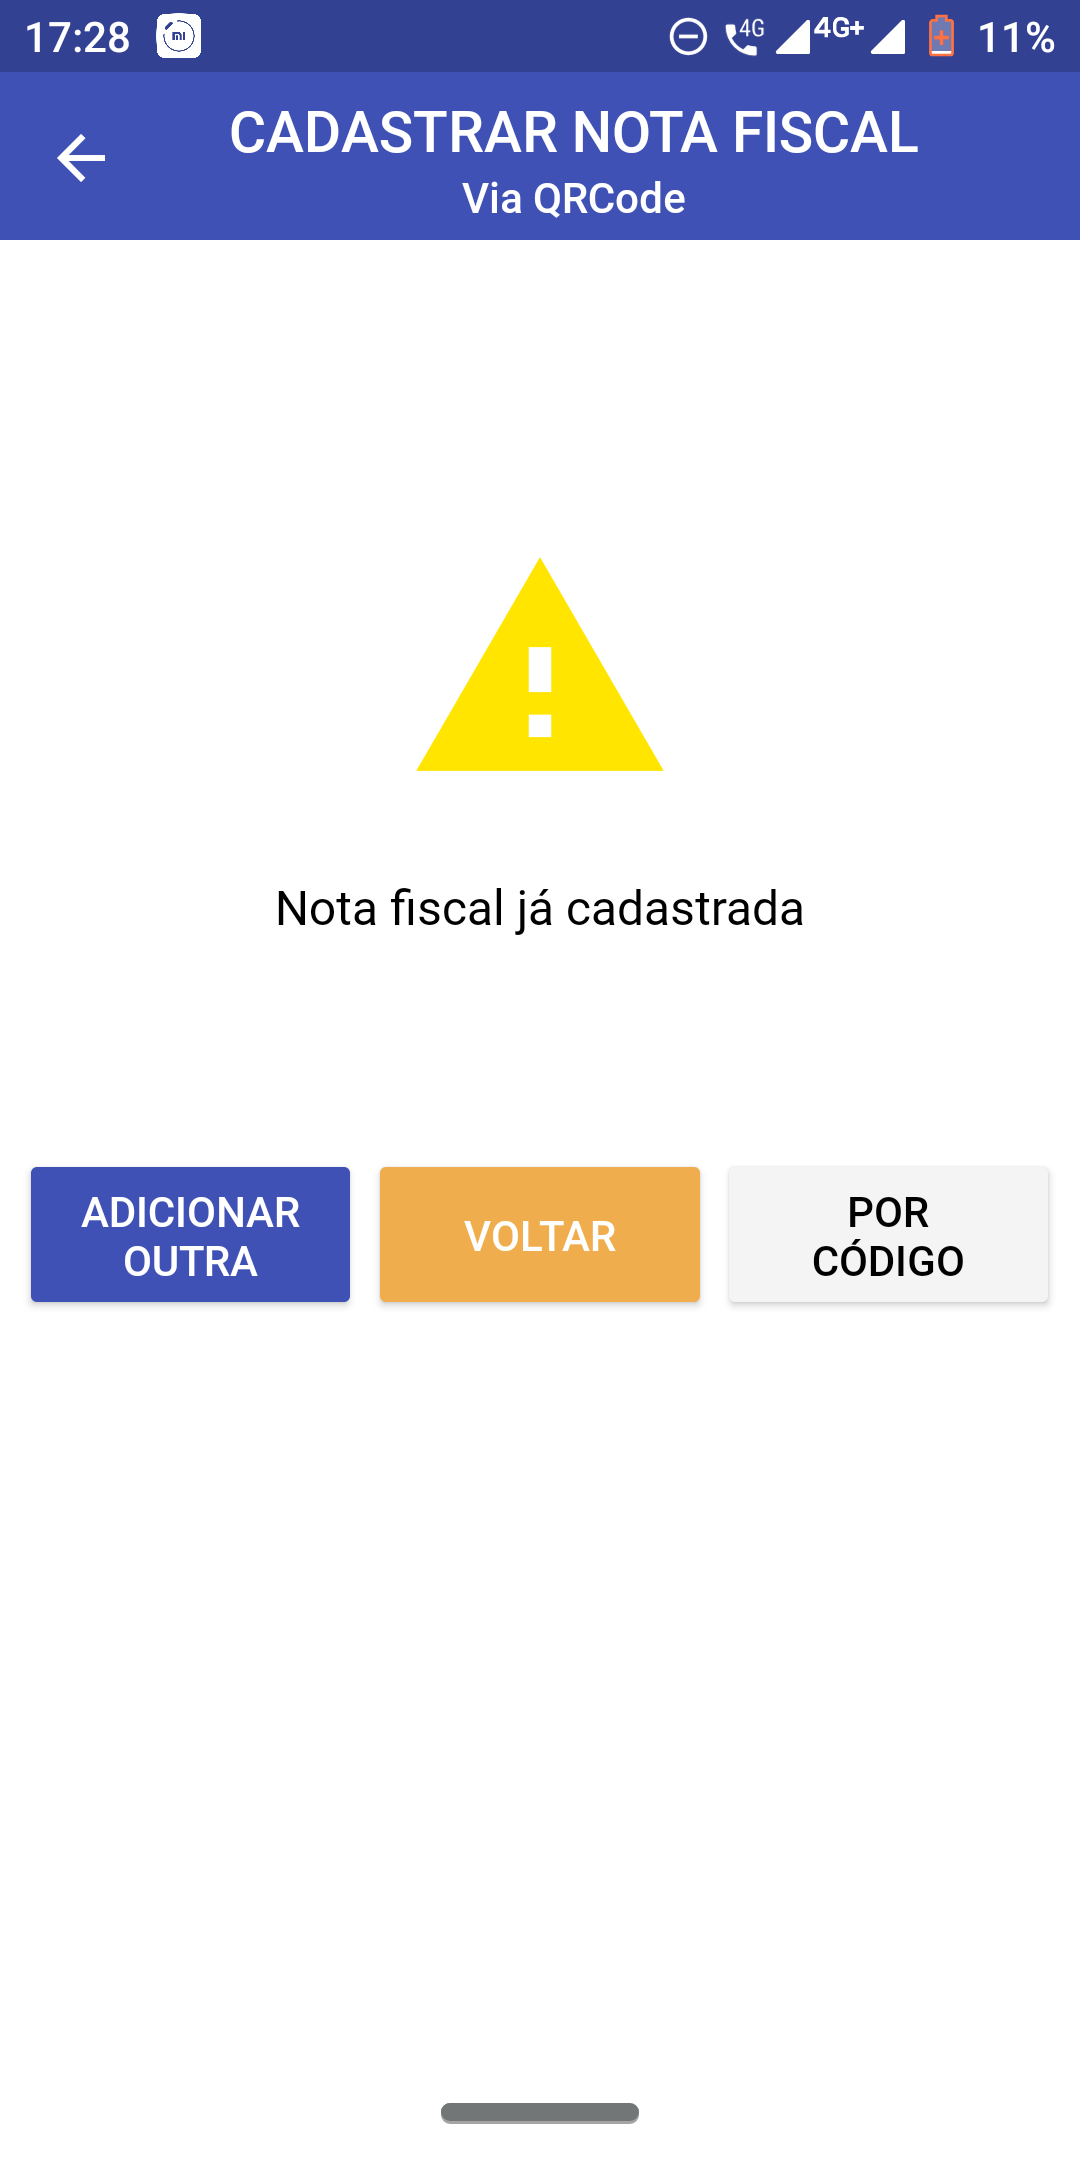
\includegraphics[scale=0.15]{tcc/figures/app/app_codigo_qrcode_ja_cadastrada.png}
    \caption{Tela de nota já cadastrada previamente}
    \label{appQRCodeJaCadastradaFig}
\end{figure}

\newpage
Durante a solicitação, está suscetível a ocorrência de erros, que pode se dar devido a problemas com a rede, problemas no sistema da SEFAZ e entre outras inúmeras situações. Diante desses erros inesperados, o usuário também é informado através de uma mensagem de erro genérica.

% FIXME: Ajustar a imagem
% FIXME: Adicionar referencia a imagem
\begin{figure}[h]
    \centering
    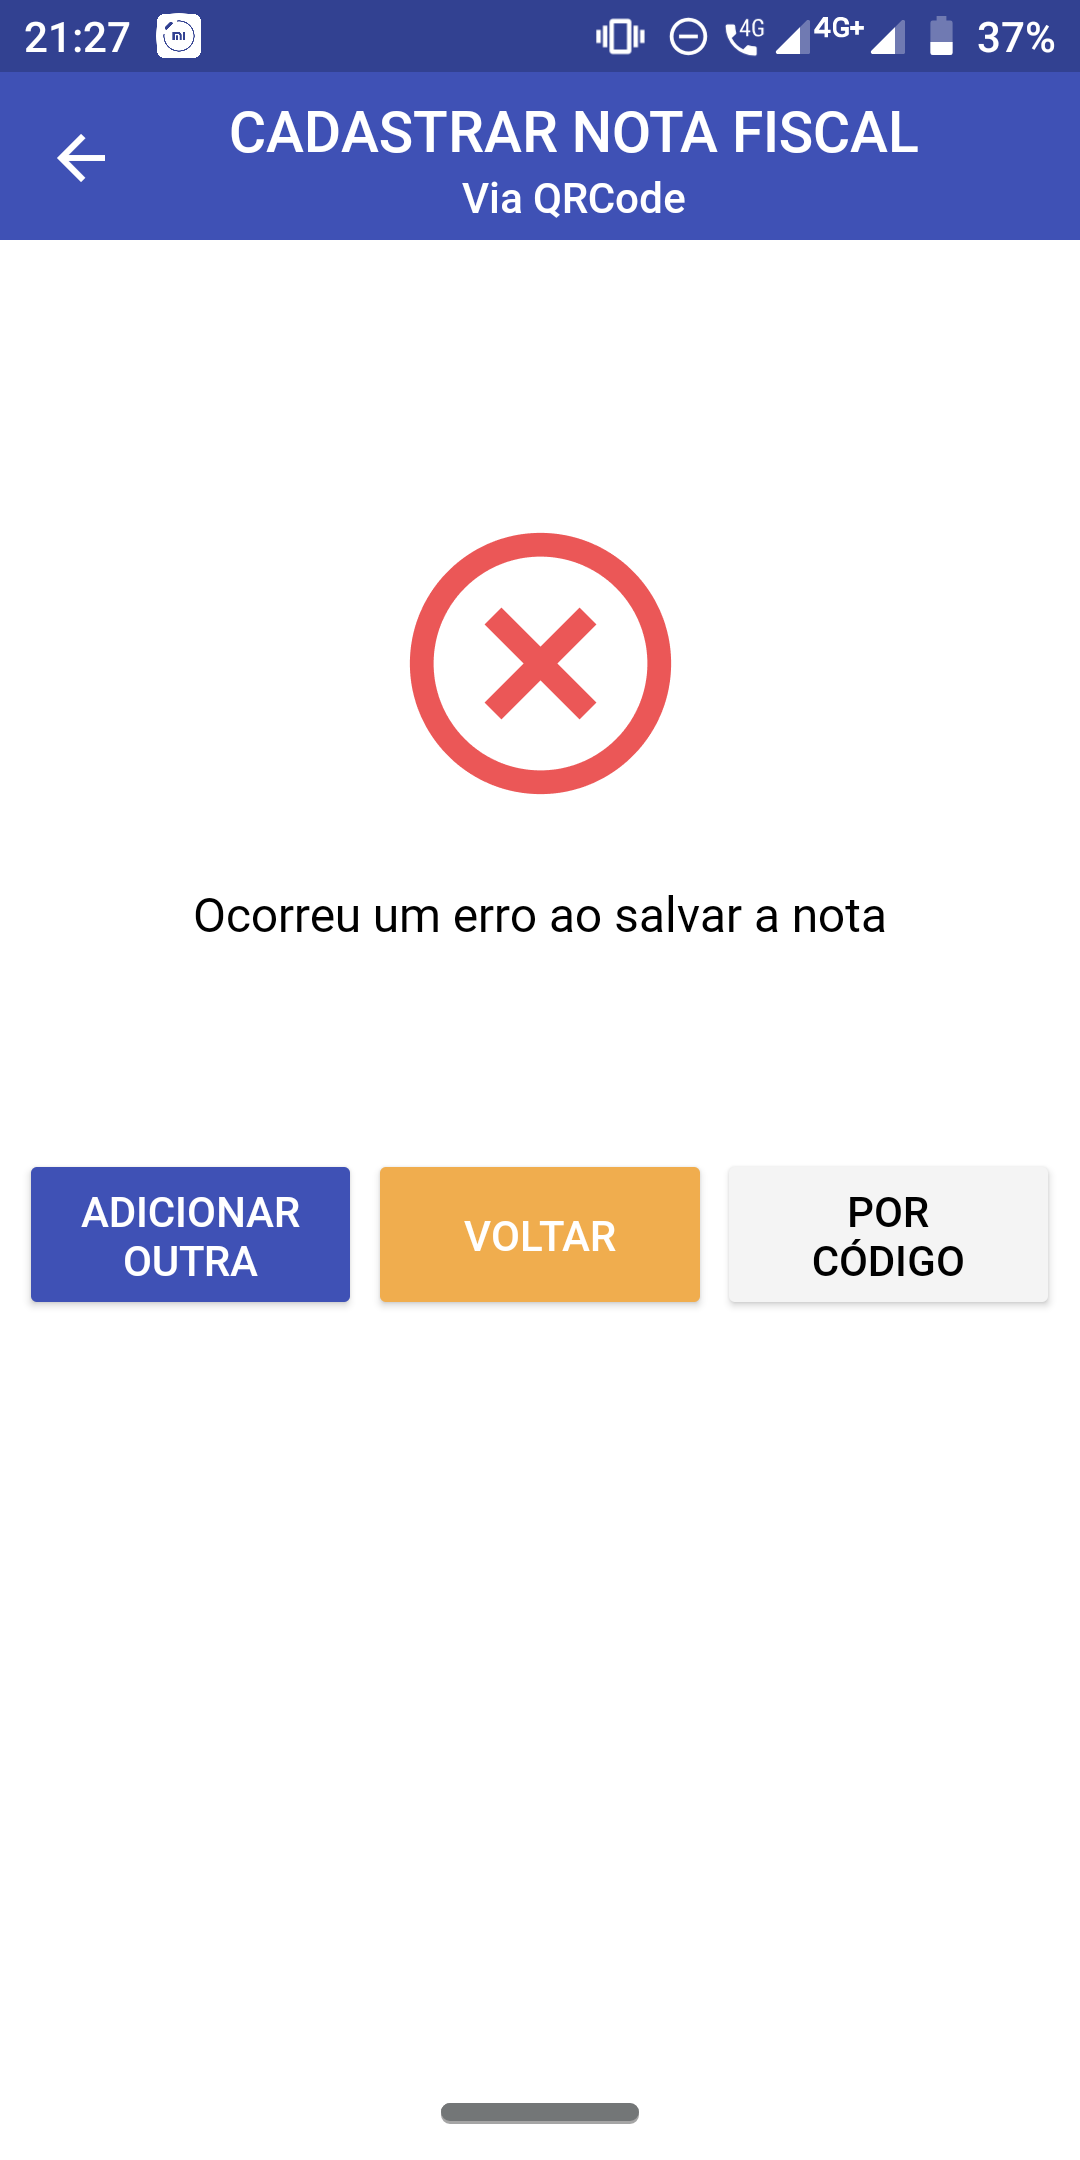
\includegraphics[scale=0.15]{tcc/figures/app/app_codigo_qrcode_erro.png}
    \caption{Tela apresentada após erro durante solicitação}
    \label{appQRCodeErroFig}
\end{figure}

\newpage
Em suma, vale destacar que, independente do caso, é apresentado ao usuário três opções, através de botões, após o término do processamento da solicitação. A primeira opção, representada pelo botão azul, permite ao usuário adicionar uma outra nota fiscal através do uso do QRCode ou até mesmo tentar adicionar a mesma nota novamente caso tenha ocorrido erros. A opção do meio, isto é, pelo botão amarelo, permite que o usuário retorne para a tela inicial. Por fim, o último botão, representa um atalho para adição através do uso do código de acesso.

\subsubsection{Através de código de acesso}

Se durante o processo de impressão da NFC-e ocorrer problemas e o QRCode não ficar nítido ou apresentar falhas, o aplicativo estará propenso a não conseguir efetuar a leitura correta da informação presente nesse código. Para contornar esse problema, é oferecida uma outra forma de adição de notas através de uma outra informação também presente na mesma, isto é, através do código de acesso.

\newpage
% FIXME: Ajustar a imagem
% FIXME: Adicionar referencia a imagem
\begin{figure}[h]
    \centering
    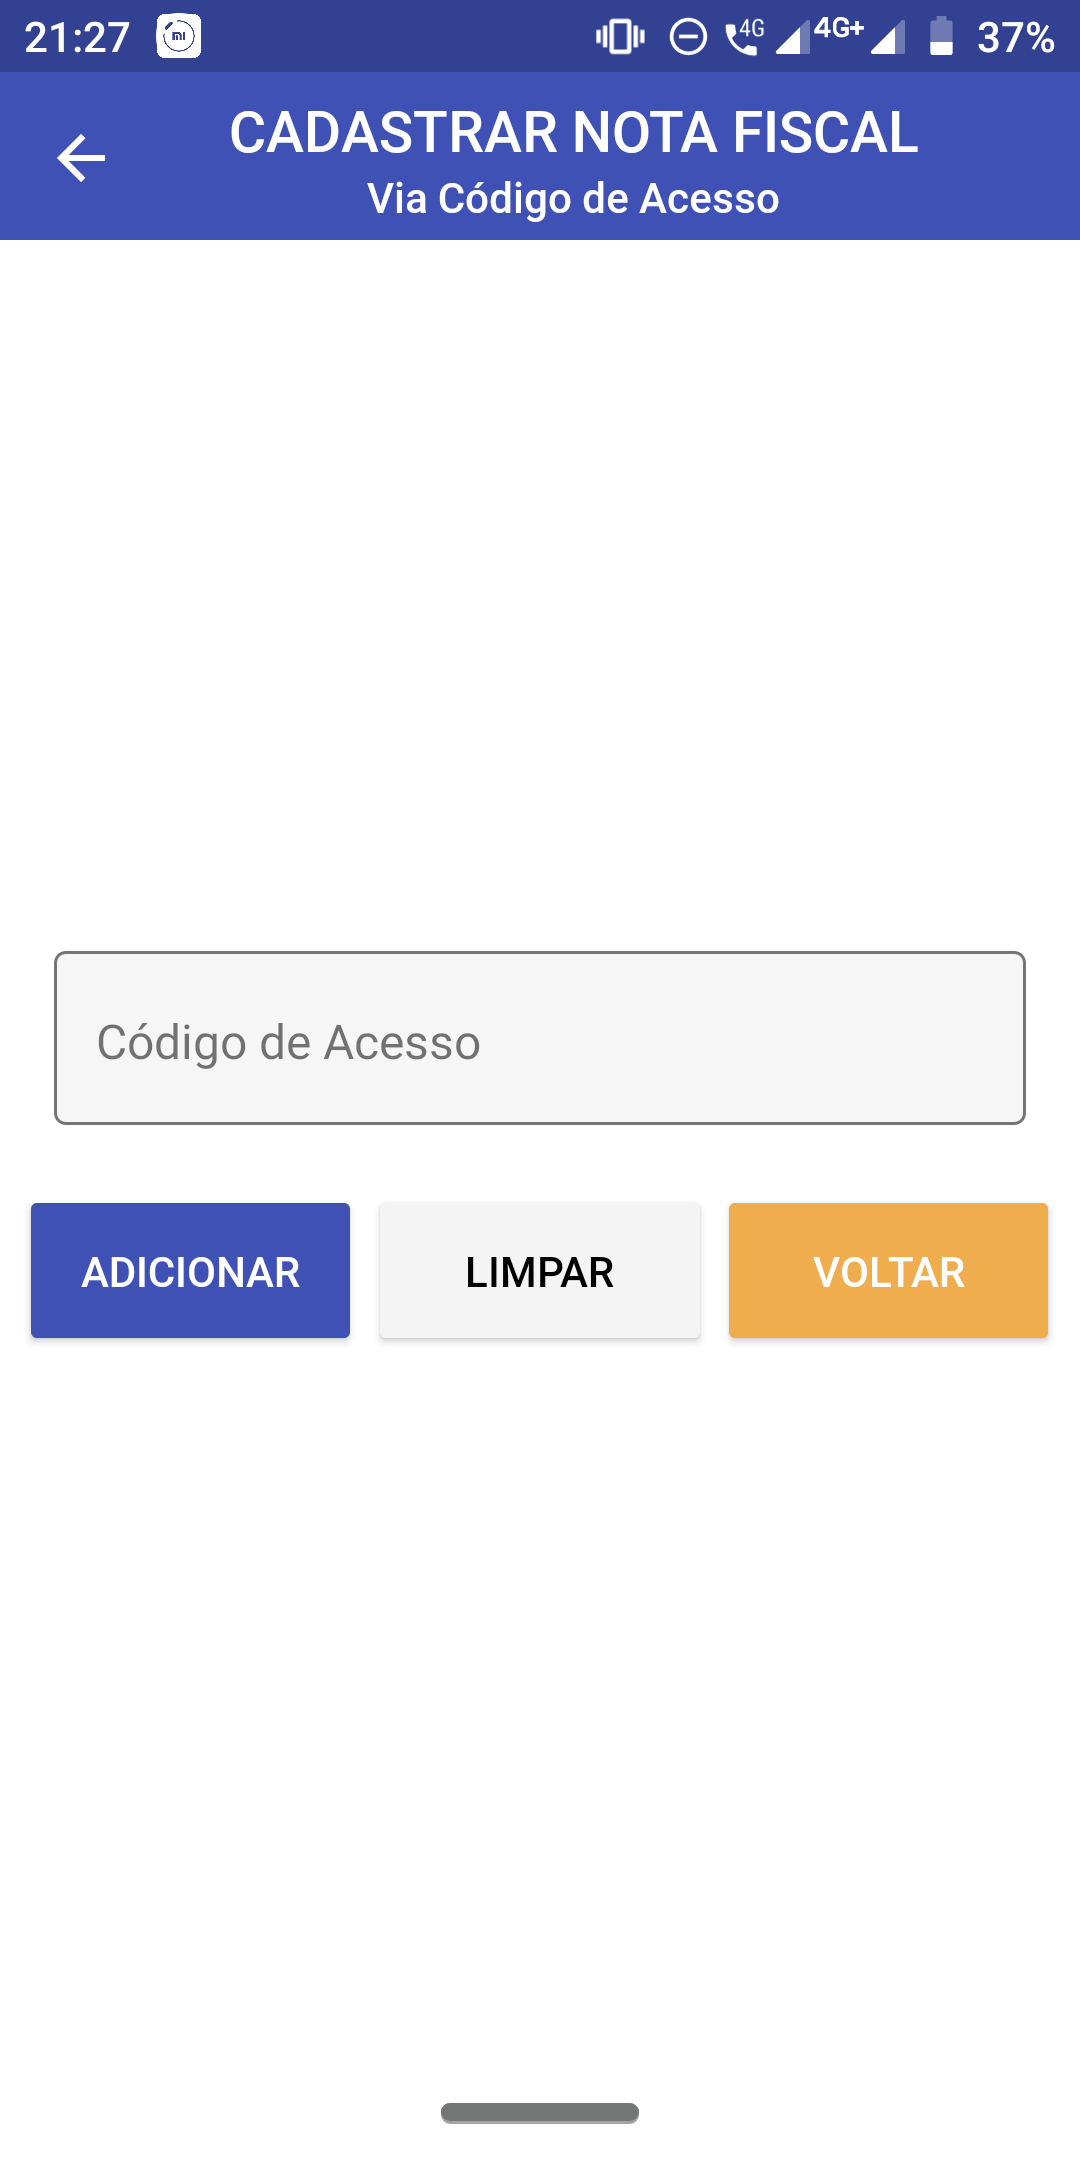
\includegraphics[scale=0.15]{tcc/figures/app/app_codigo_acesso.png}
    \caption{Tela inicial do cadastro via código de acesso}
    \label{appCodigoAcessoInicialFig}
\end{figure}

A figura \ref{appCodigoAcessoInicialFig} representa a tela inicial de cadastro efetuado através do uso do código de acesso. O primeiro campo é para a inserção do código que é necessário para solicitação. Abaixo desse campo, encontram-se os botões para a interação do usuário. O primeiro botão, em azul, é para a inicialização do processo de adição. Caso o usuário não insira a quantidade necessária de dígitos, o sistema irá notificar o usuário sobre esse problema. O botão do meio, em branco, permite a limpeza total do texto inserido. Por último, o botão mais à direita serve como atalho para o usuário retornar à tela inicial.

\newpage
% FIXME: Ajustar a imagem
% FIXME: Adicionar referencia a imagem
\begin{figure}[h]
    \centering
    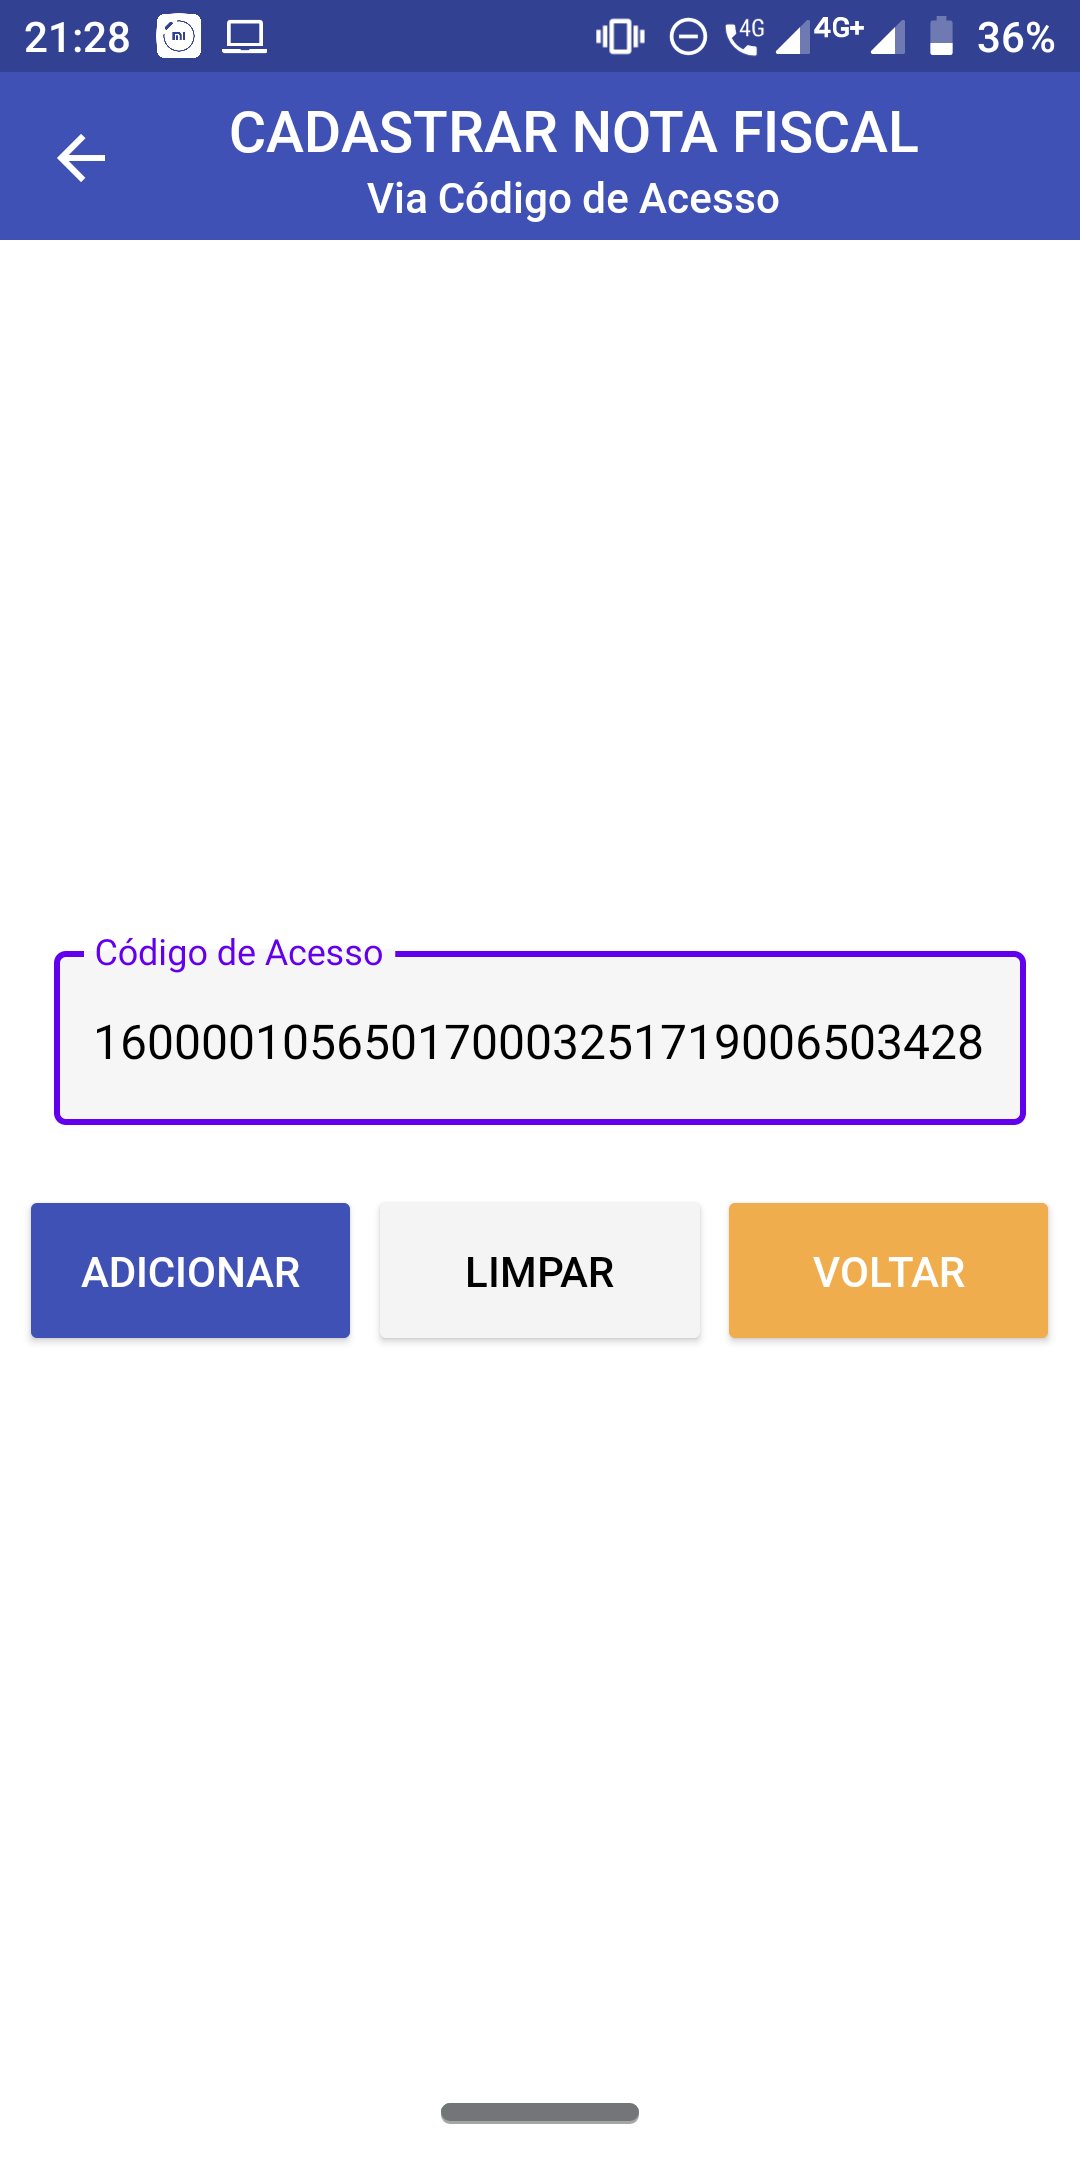
\includegraphics[scale=0.15]{tcc/figures/app/app_codigo_acesso_com_codigo.png}
    \caption{Tela de cadastro via código de acesso com código inserido}
    \label{appCodigoAcessoComCodigoFig}
\end{figure}

% FIXME: Ajustar a imagem
% FIXME: Adicionar referencia a imagem
\begin{figure}[h]
    \centering
    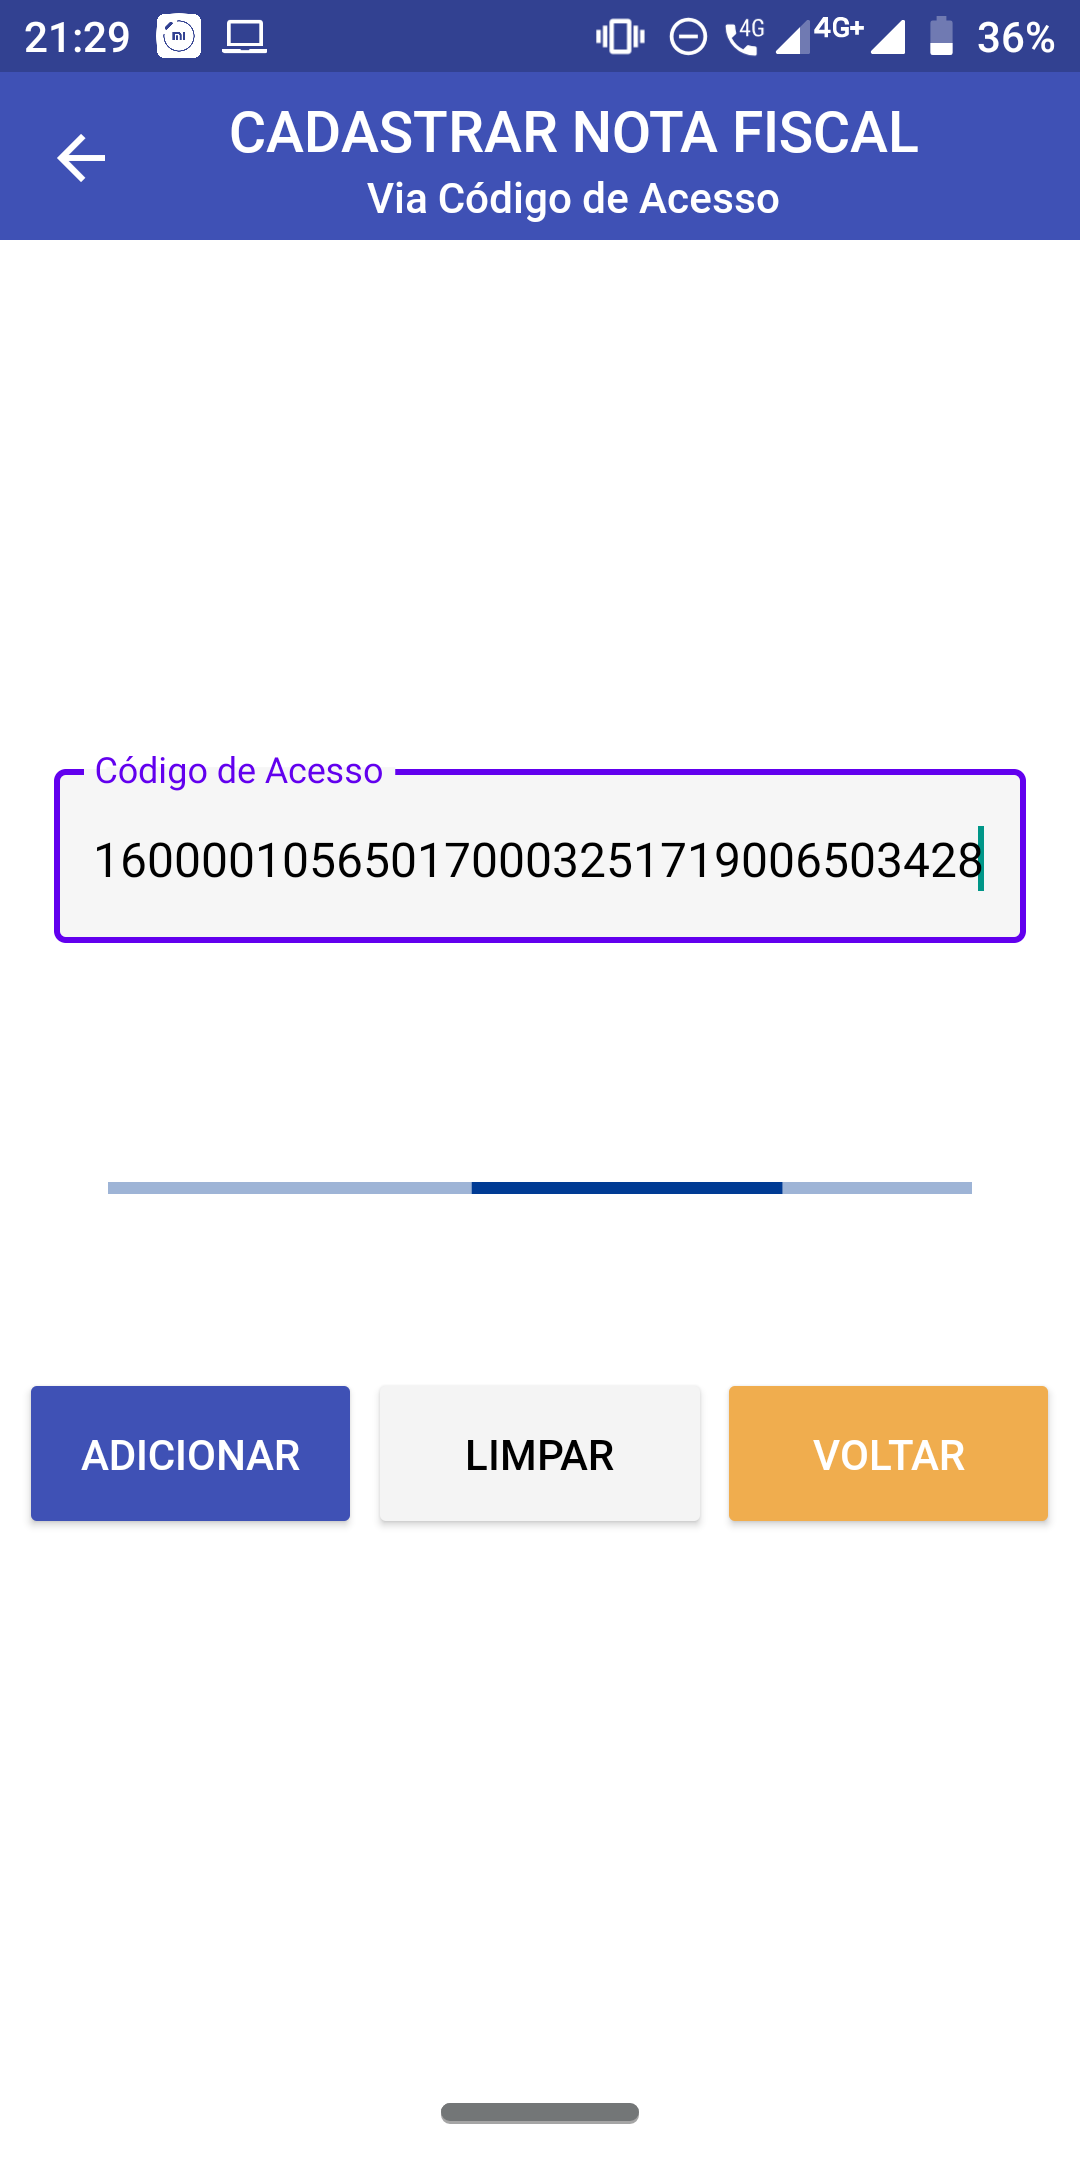
\includegraphics[scale=0.15]{tcc/figures/app/app_codigo_acesso_loading.png}
    \caption{Tela de cadastro via código de acesso com carregamento}
    \label{appCodigoAcessoCarregamentoCaptchaFig}
\end{figure}

\newpage
Após a inserção do código de acesso e o usuário ter pressionado o botão de adicionar, será mostrado o CAPTCHA para validação da requisição. Esse código é necessário para comprovação que a solicitação é proveniente de interação humana e não foi feita por sistemas automáticos. Essa validação pertence ao sistema da SEFAZ e o aplicativo simplesmente replica a mesma imagem utilizada por esse sistema para que a solicitação efetuada no site possa ser simulada. Como essa imagem precisa ser transferida para o aplicativo, uma barra de progresso é exibida até que a imagem seja baixada em sua totalidade conforme é explicitado pela Figura \ref{appCodigoAcessoCarregamentoCaptchaFig}. Além da imagem representativa desse código de validação, um campo destinado a inserção do texto referente a essa mesma imagem são acrescentados à tela anterior. A figura \ref{appCodigoAcessoCaptchaFig} exemplifica esse fluxo descrito.

Vale destacar, que os mesmos botões disponíveis na tela anterior (Figura \ref{appCodigoAcessoComCodigoFig}) ainda estão presentes, todavia, o botão de adicionar deverá ser utilizado após a inserção do texto referente ao CAPTCHA, já o botão limpar serve para limpeza do campo destinado a inserção desse mesmo texto.

\newpage
% FIXME: Ajustar a imagem
% FIXME: Adicionar referencia a imagem
\begin{figure}[h]
    \centering
    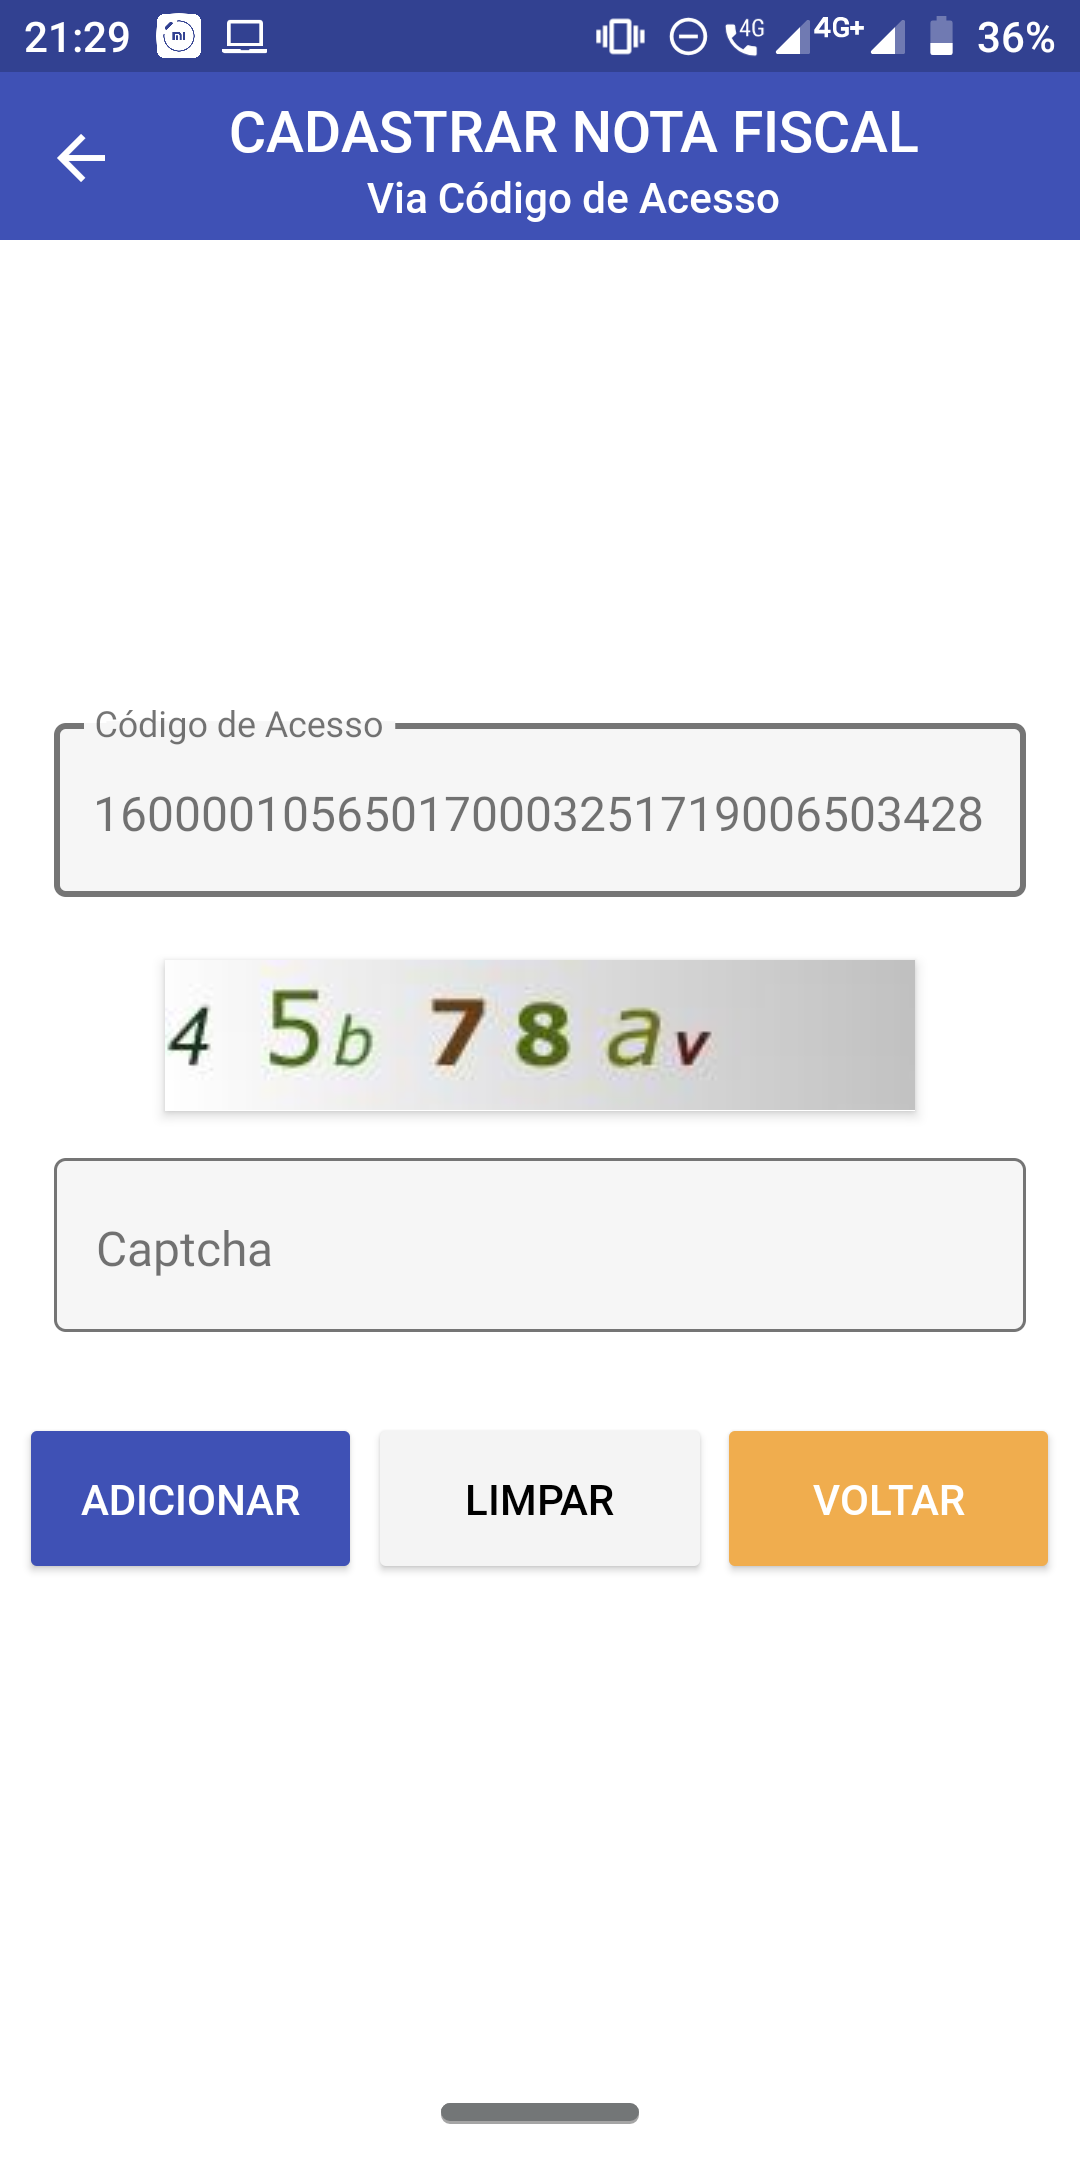
\includegraphics[scale=0.15]{tcc/figures/app/app_codigo_acesso_captcha.png}
    \caption{Tela de cadastro solicitando CAPTCHA para validação da requisição}
    \label{appCodigoAcessoCaptchaFig}
\end{figure}

Assim como ocorre com o cadastro via QRCode, alguns segundos serão gastos até o término do processamento dos dados, com isso, uma tela com uma barra de progresso também é exibida até o resultado da solicitação ser retornado ao aplicativo.

\newpage
% FIXME: Ajustar a imagem
% FIXME: Adicionar referencia a imagem
\begin{figure}[h]
    \centering
    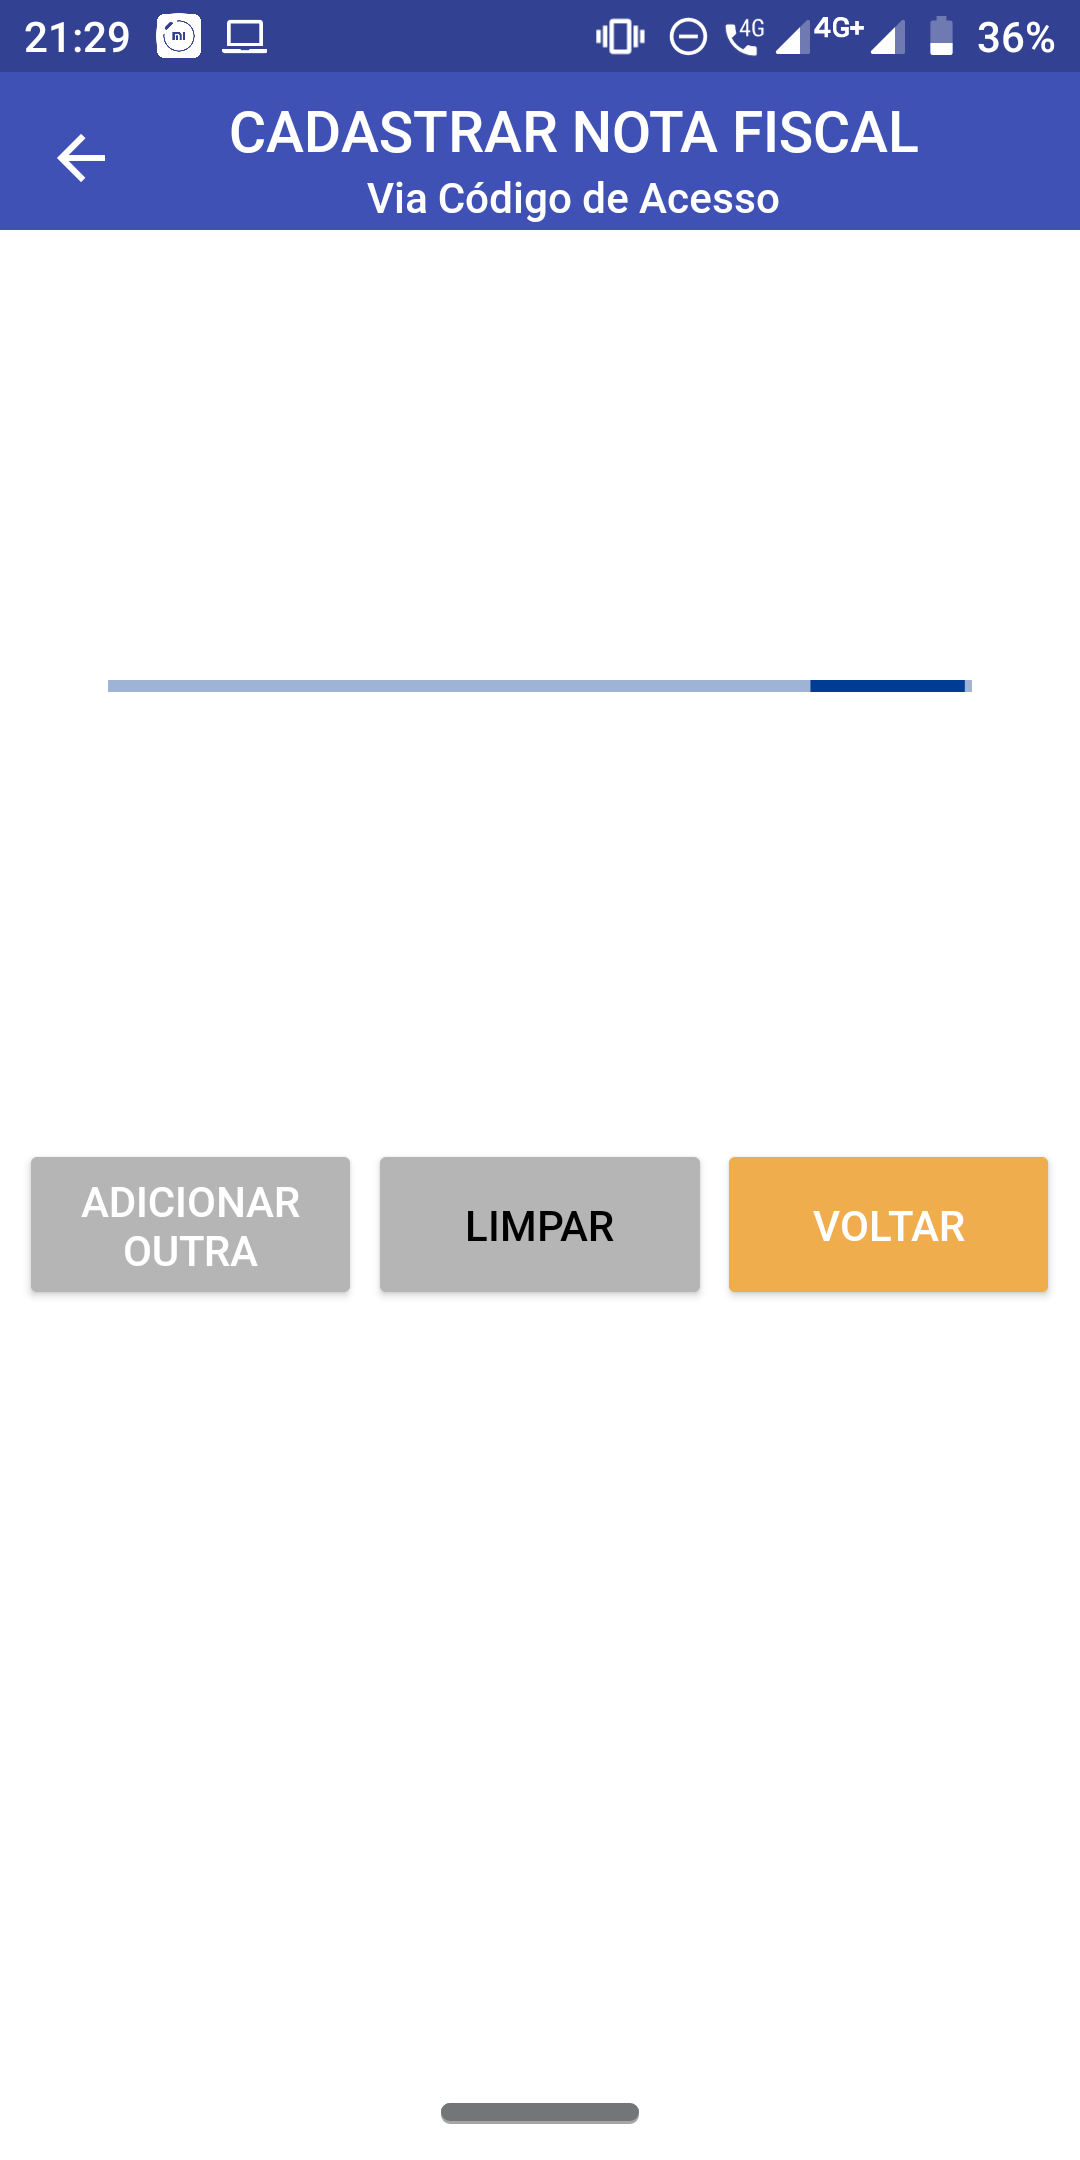
\includegraphics[scale=0.15]{tcc/figures/app/app_codigo_acesso_loading_solicitacao.png}
    \caption{Tela de cadastro via código de acesso após solicitação}
    \label{appCodigoAcessoLoadingSolicitacaoFig}
\end{figure}

Ao receber a resposta, o aplicativo irá mostrar diferentes telas dependendo do que resultado obtido. As telas são semelhantes ao serem comparadas com o outro método de adição de notas. No entanto, a principal diferença é que as telas para esse tipo de adição, os botões são diferentes. A primeira opção, também em azul, permite adicionar outra nota também por meio do código de acesso. O botão do meio, de limpar, é exibido de forma bloqueada pois não existem campos de inserção de dados nessa parte de resultados. Por fim, o último botão, em amarelo, permite que o usuário retorne para a tela inicial da aplicação.

\newpage
% FIXME: Ajustar a imagem
% FIXME: Adicionar referencia a imagem
\begin{figure}[h]
    \centering
    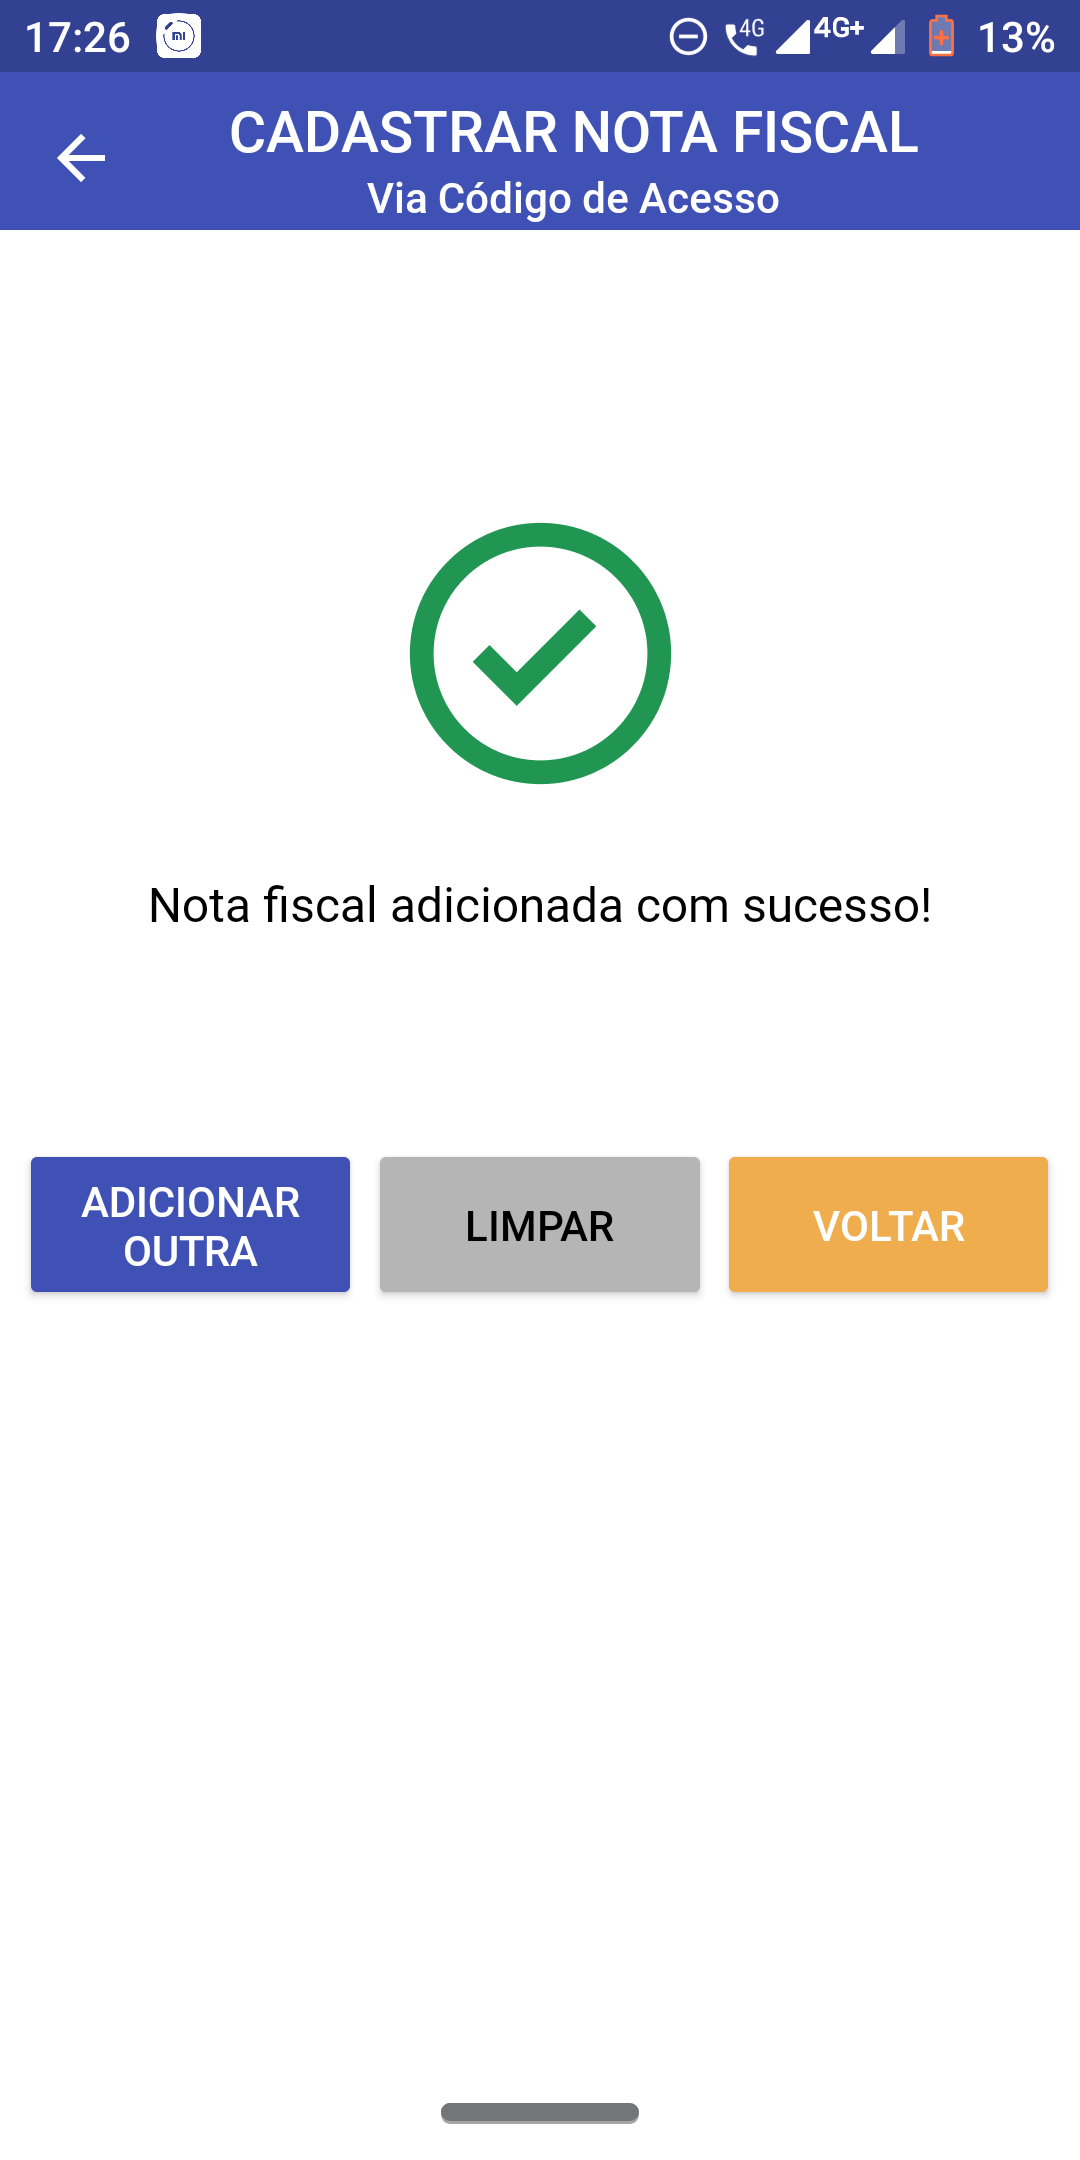
\includegraphics[scale=0.15]{tcc/figures/app/app_codigo_acesso_sucesso.png}
    \caption{Tela de cadastramento via código de acesso efetuado com sucesso}
    \label{appCodigoAcessoSucessoFig}
\end{figure}

\newpage
% FIXME: Ajustar a imagem
% FIXME: Adicionar referencia a imagem
\begin{figure}[h]
    \centering
    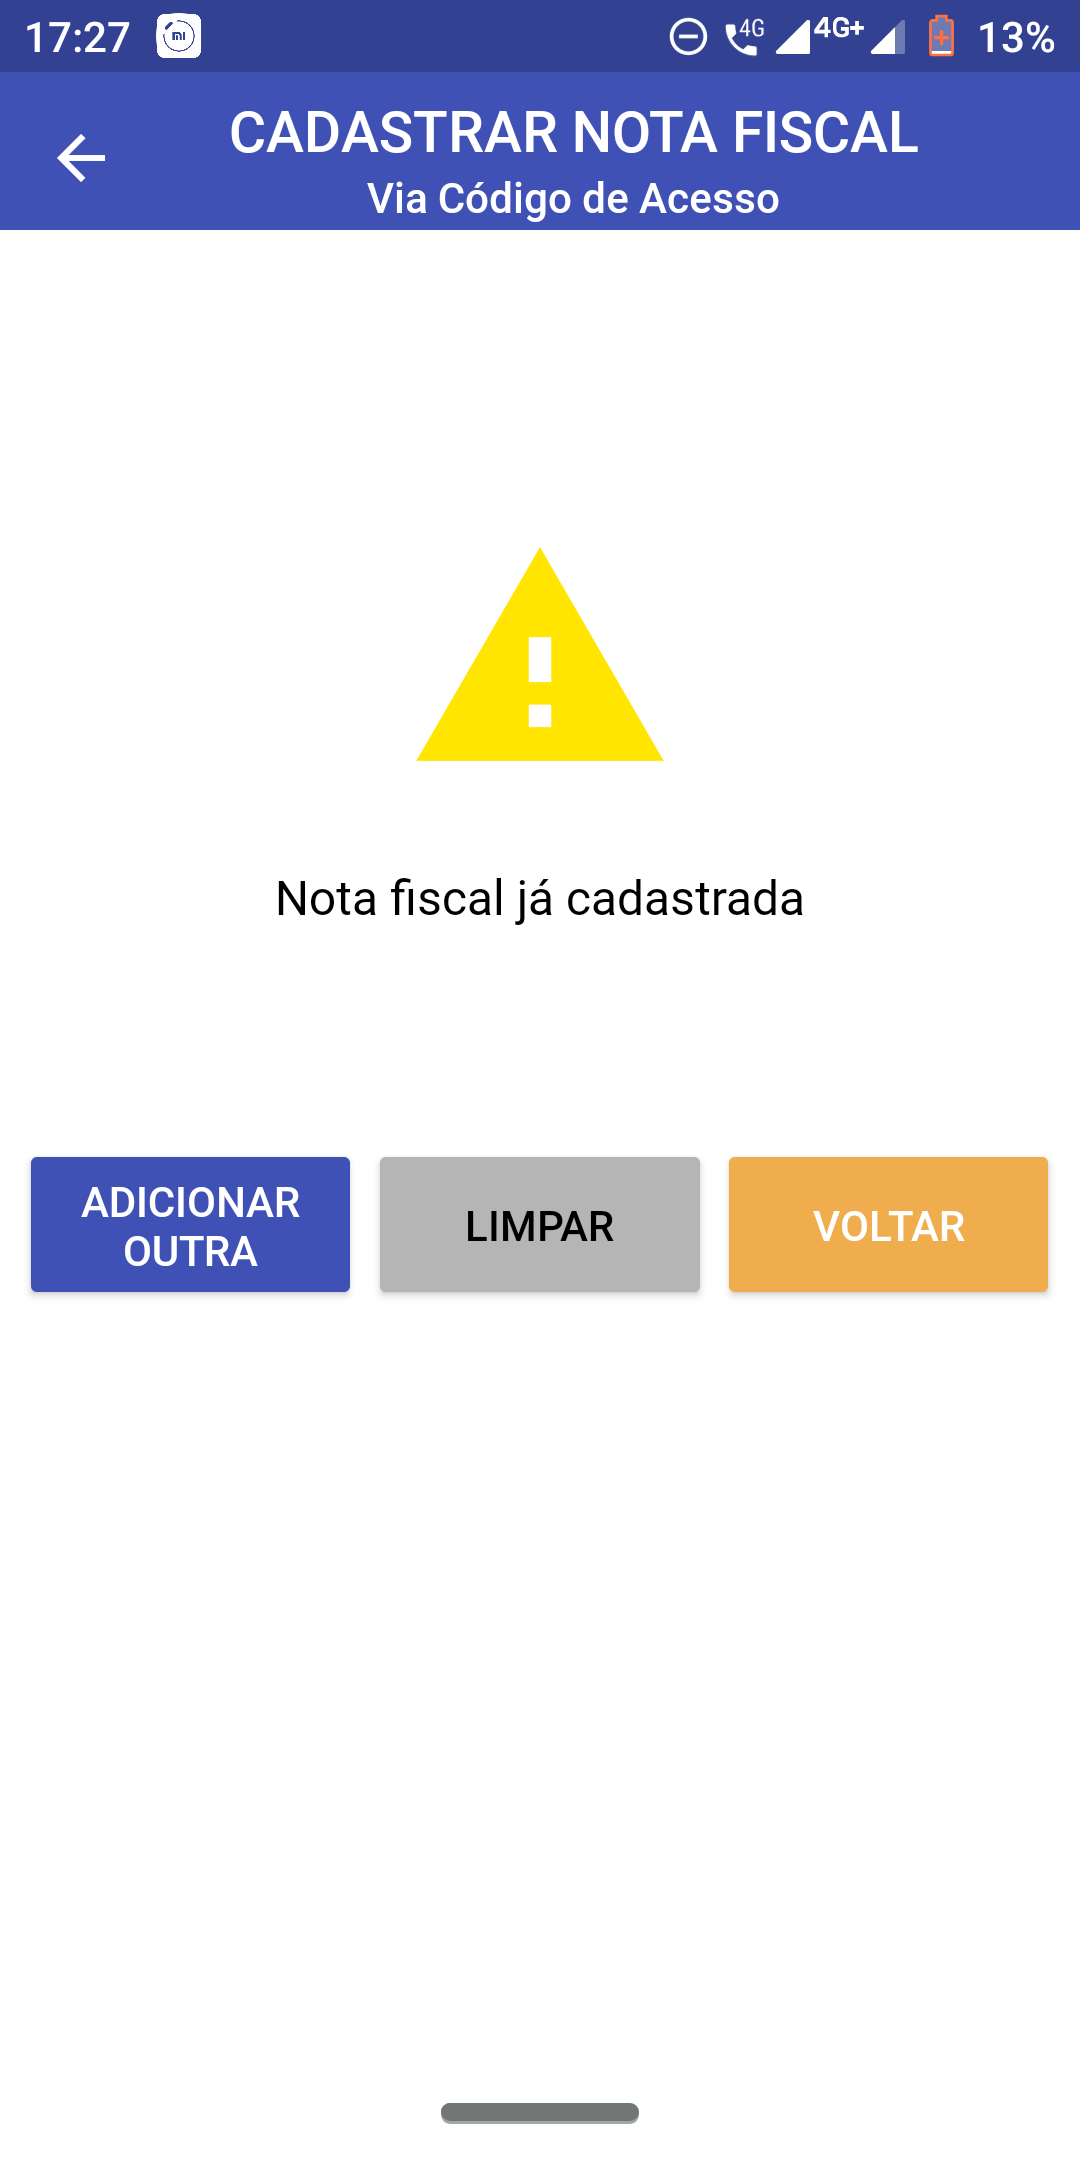
\includegraphics[scale=0.15]{tcc/figures/app/app_codigo_acesso_ja_cadastrada.png}
    \caption{Tela de cadastramento via código de acesso de uma nota cadastrada previamente}
    \label{appCodigoAcessoJaCadastradaFig}
\end{figure}

\newpage
% FIXME: Ajustar a imagem
% FIXME: Adicionar referencia a imagem
\begin{figure}[h]
    \centering
    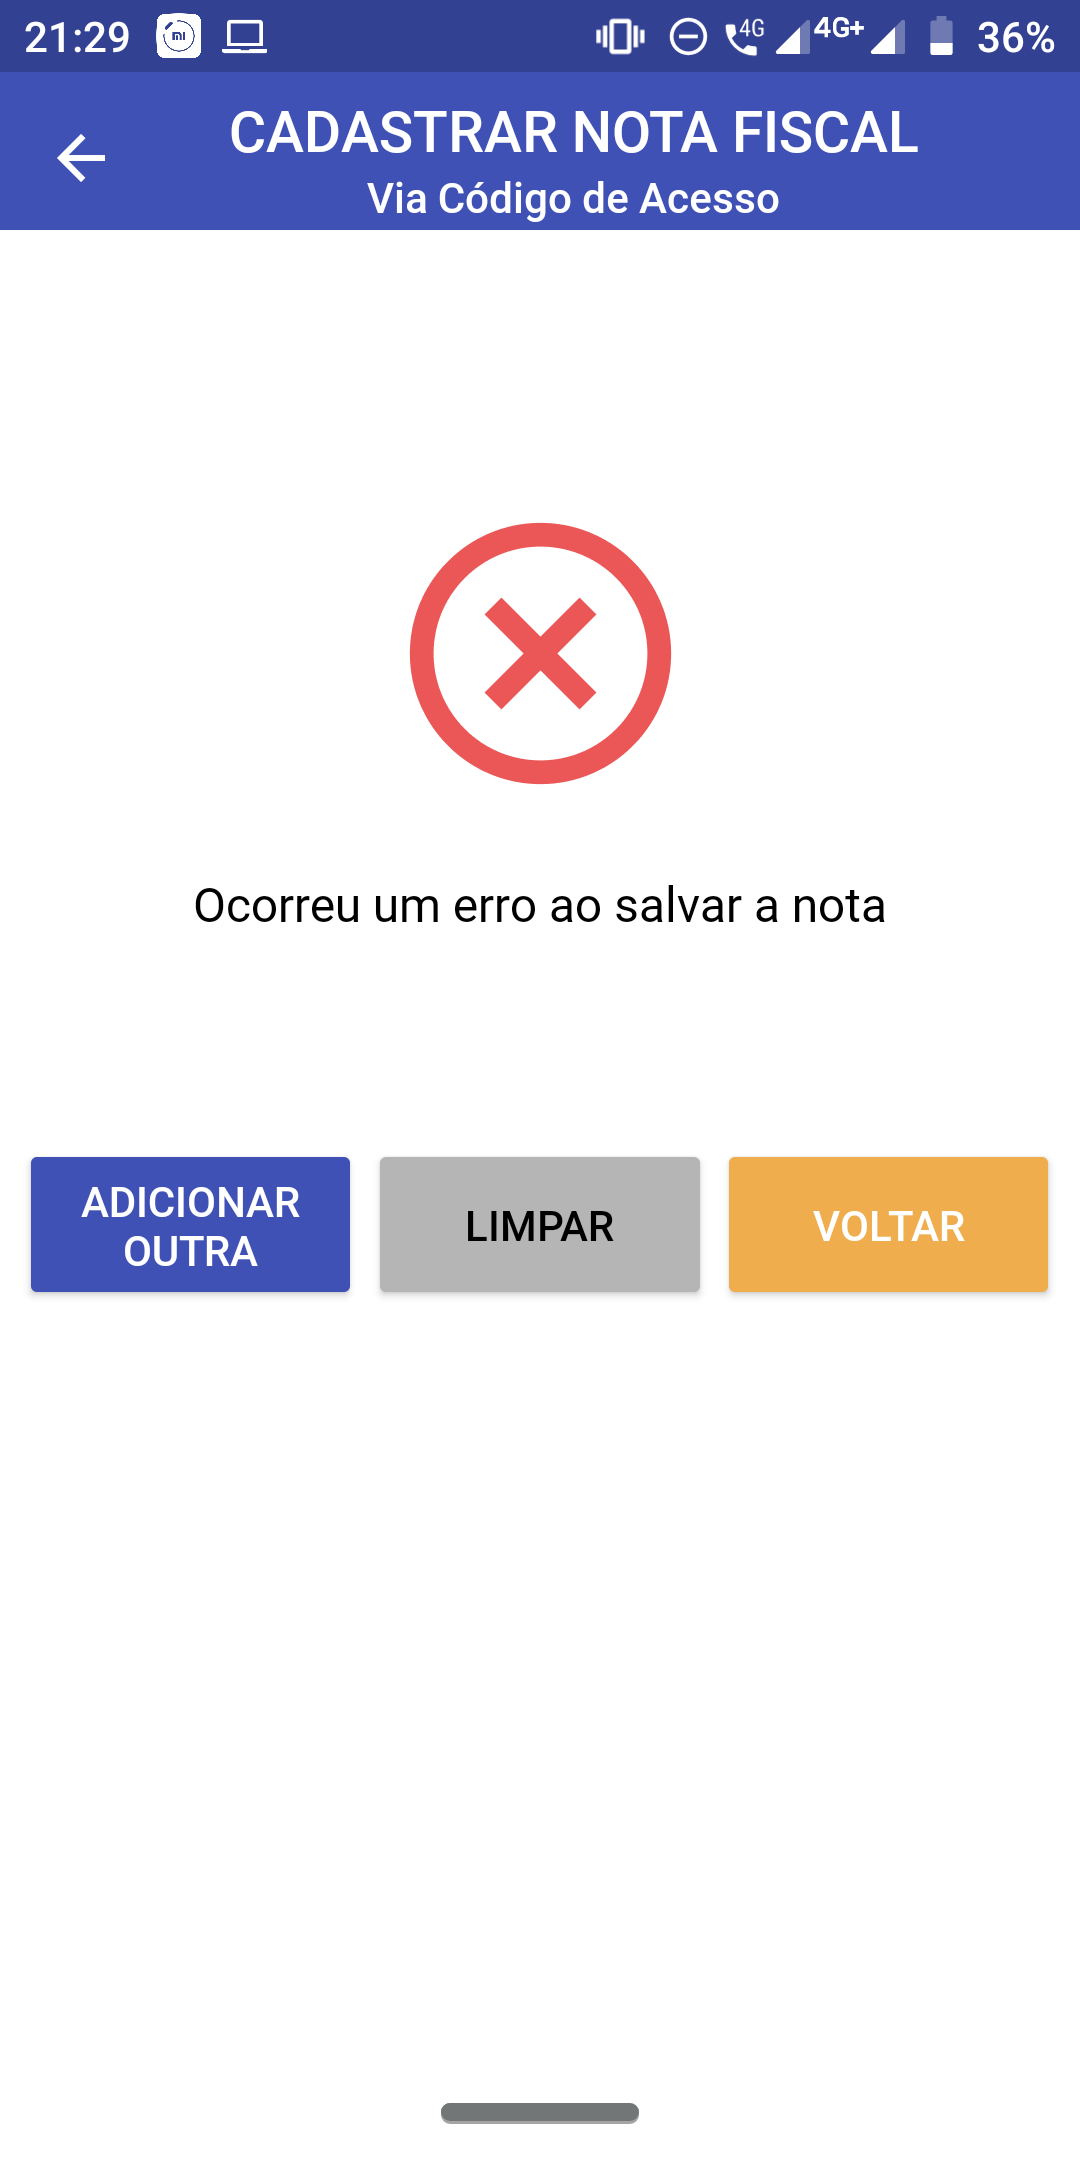
\includegraphics[scale=0.15]{tcc/figures/app/app_codigo_acesso_nao_disponivel.png}
    \caption{Tela de cadastramento via código de acesso de uma nota não disponível}
    \label{appCodigoAcessoNaoDisponivelFig}
\end{figure}

\newpage
% FIXME: Ajustar a imagem
% FIXME: Adicionar referencia a imagem
\begin{figure}[h]
    \centering
    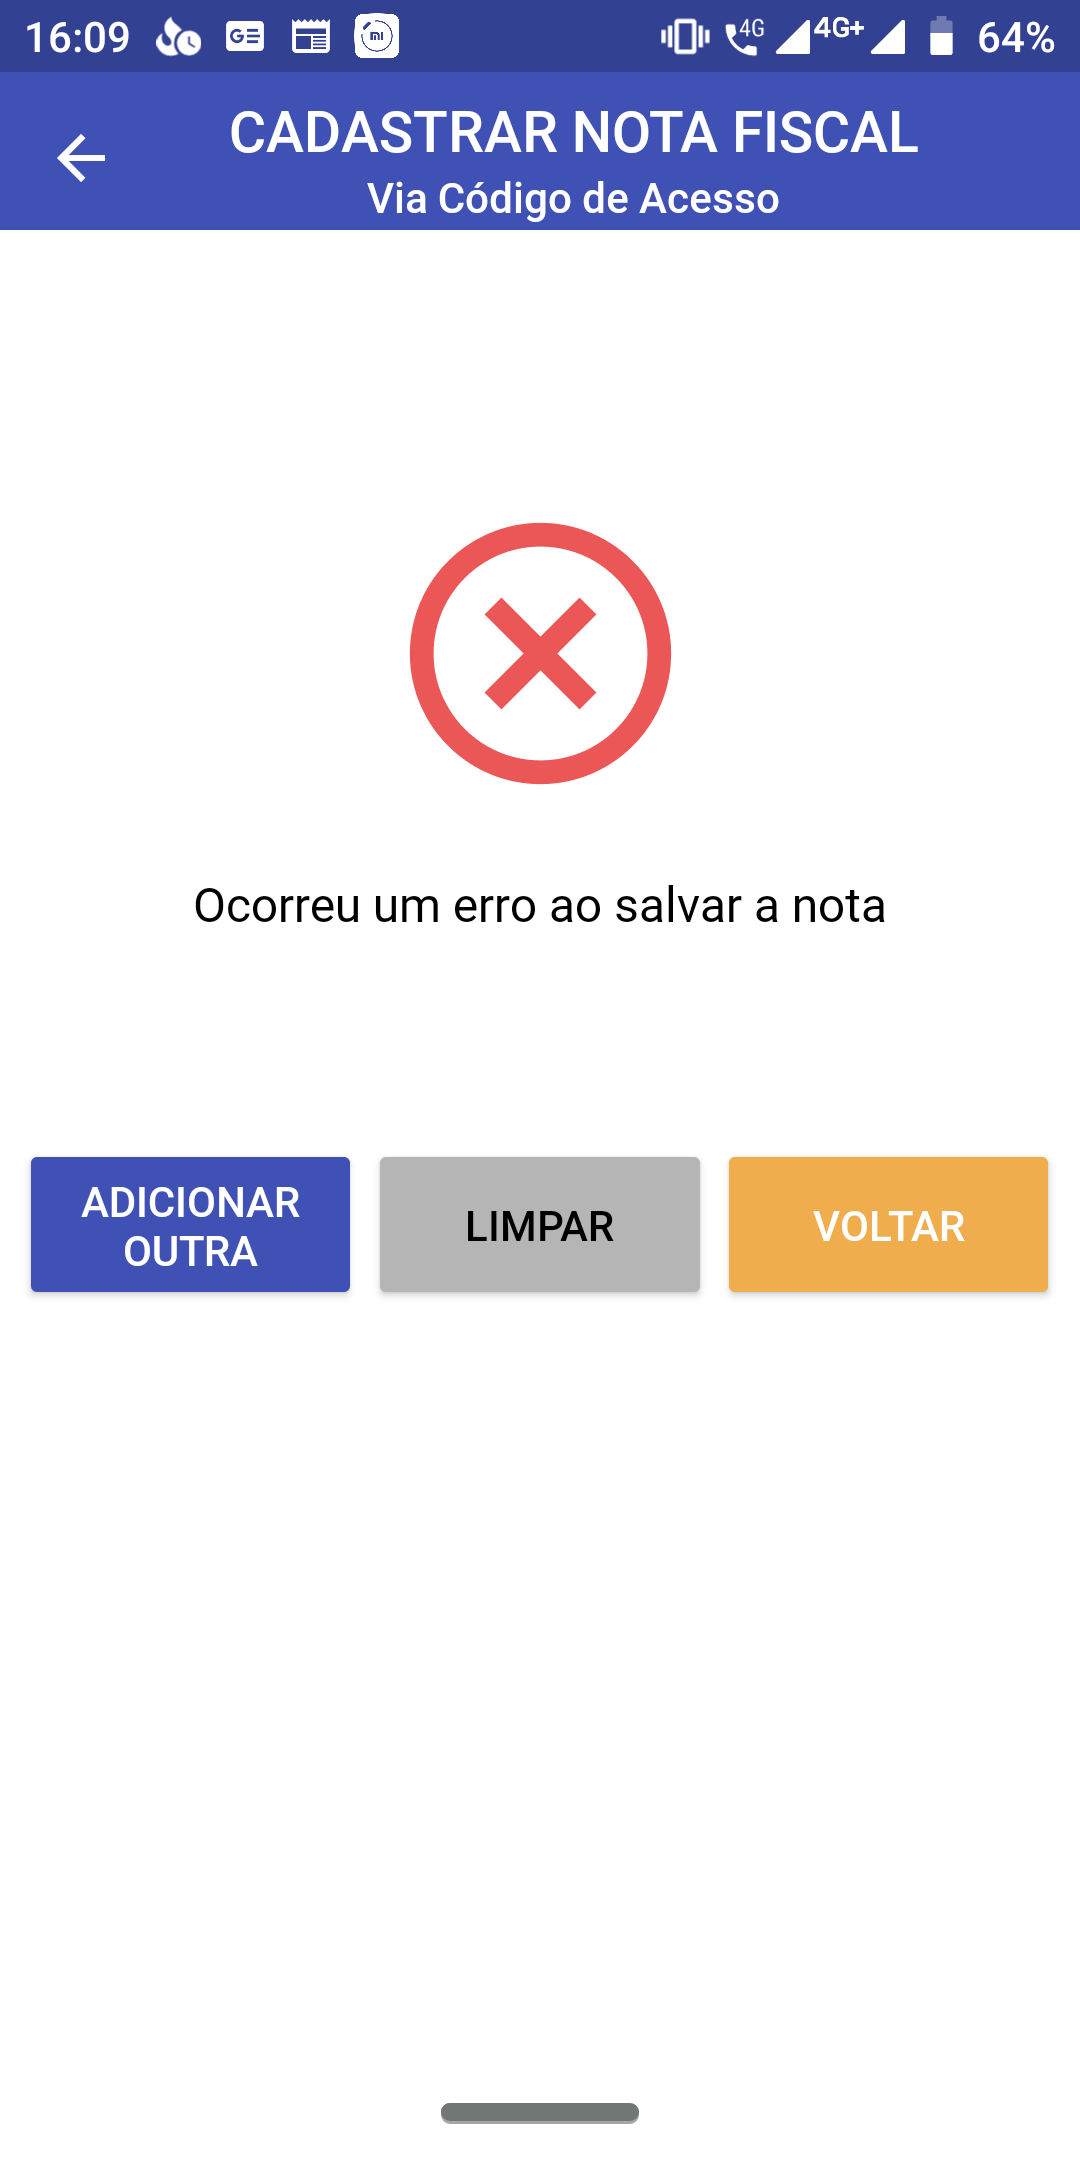
\includegraphics[scale=0.15]{tcc/figures/app/app_codigo_acesso_erro_generico.png}
    \caption{Tela de cadastramento via código de acesso após erro durante solicitação}
    \label{appCodigoAcessoErroFig}
\end{figure}

\newpage
% FIXME: Ajustar a imagem
% FIXME: Adicionar referencia a imagem
\begin{figure}[h]
    \centering
    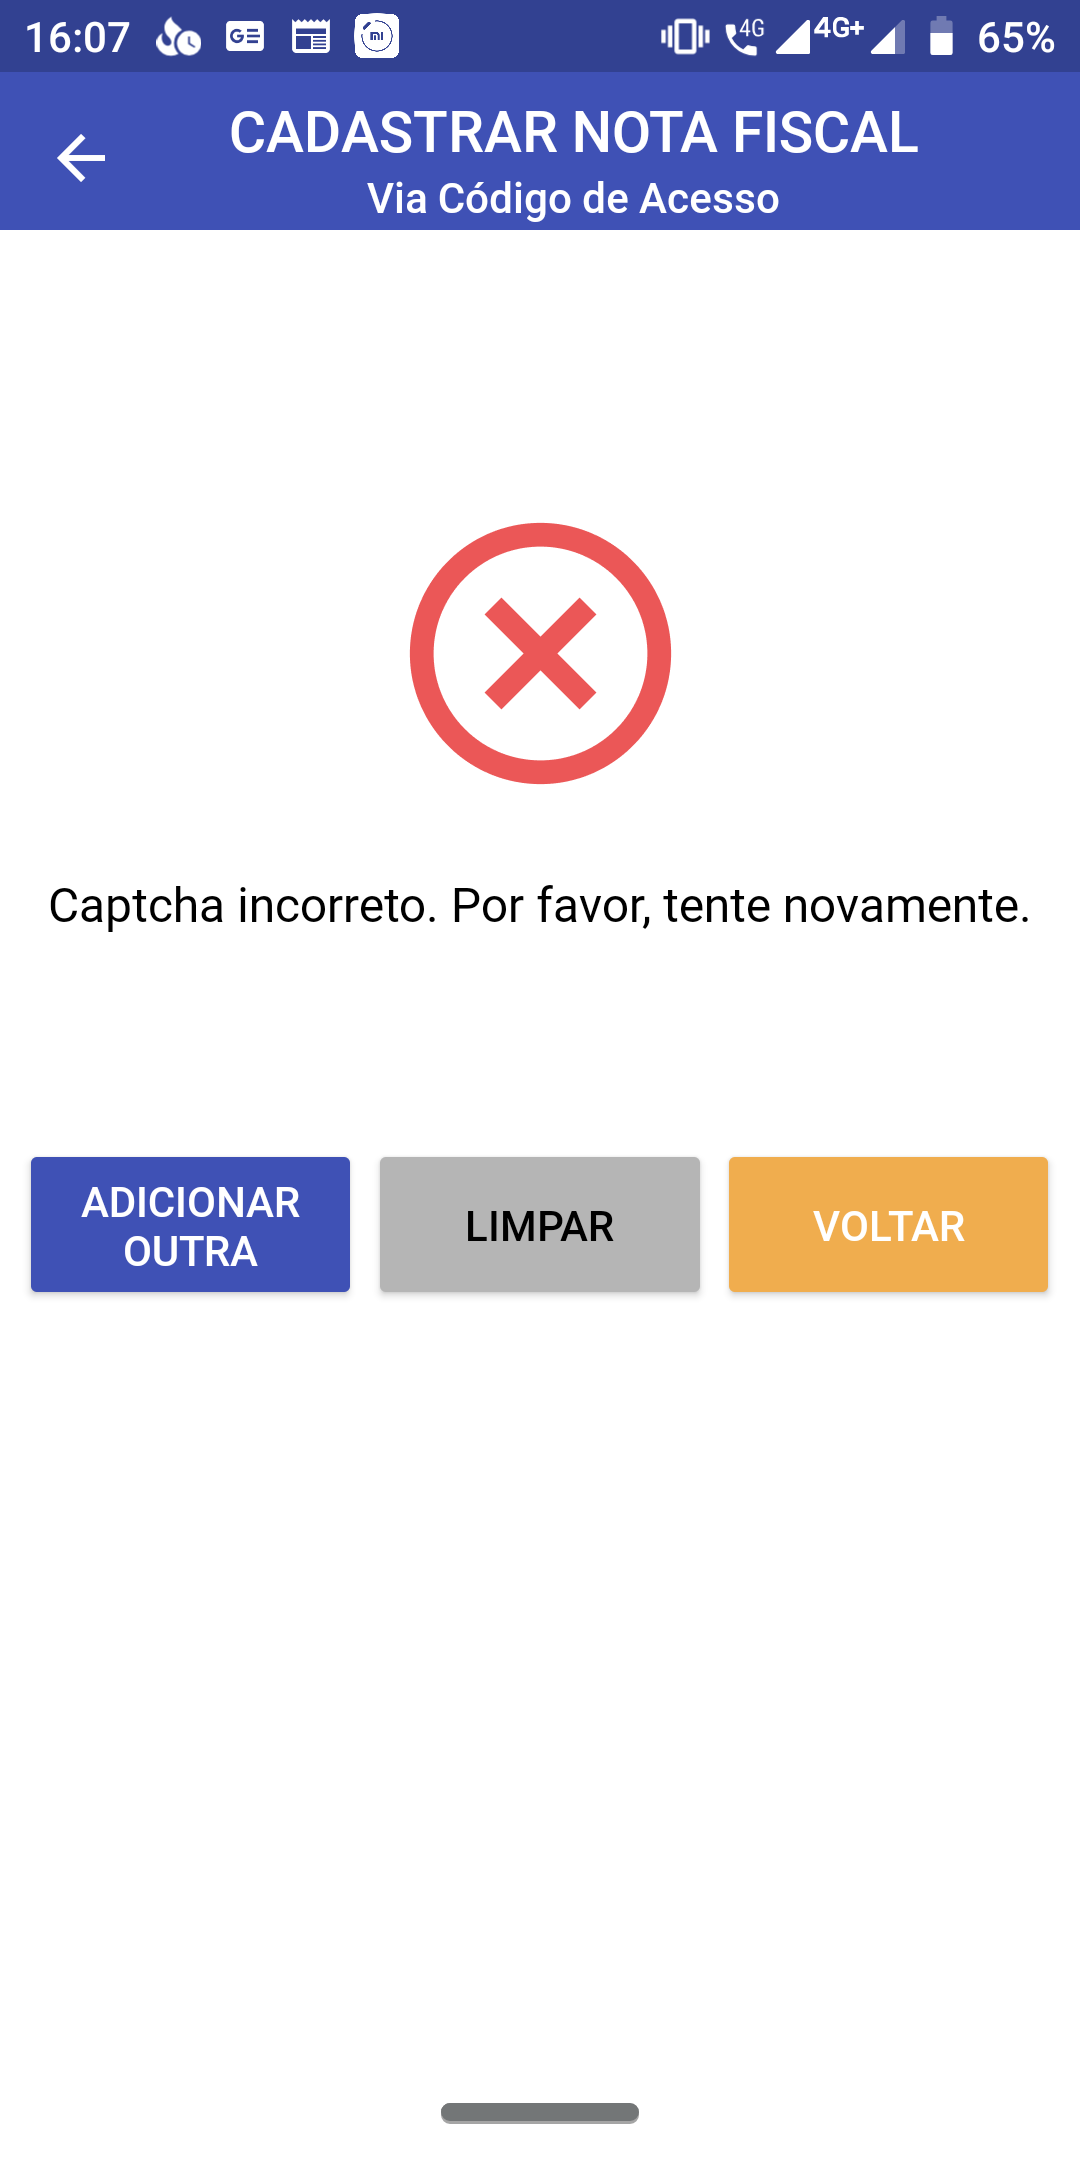
\includegraphics[scale=0.15]{tcc/figures/app/app_codigo_acesso_erro_captcha.png}
    \caption{Tela de cadastramento via código de acesso após inserção falha no teste do CAPTCHA}
    \label{appCodigoAcessoErroCaptchaFig}
\end{figure}

Existe uma tela diferente das demais quando comparado aos resultados do cadastro via QRCode. Isso ocorre devido a presença do campo para inserção do CAPTCHA, com isso deverá ter um tratamento para o erro do caso em que o usuário tenha inserido um texto diferente daquele presente na imagem. Esse erro resulta em uma falha no teste de validação, o que impede o término do processo de cadastro via esse meio.

\subsection{Busca de produtos}

Ao clicar no último botão da tela inicial, conforme visto na figura \ref{appHomeFig}, o usuário será encaminhado para a tela de busca de produtos. É através dessa tela que os usuários poderão consultar a informação referente aos produtos desejados cadastrados previamente. A tela em questão é apresentada pela figura \ref{appBuscaProdutosInicialFig}.

% FIXME: Ajustar a imagem
% FIXME: Adicionar referencia a imagem
\newpage
\begin{figure}[h]
    \centering
    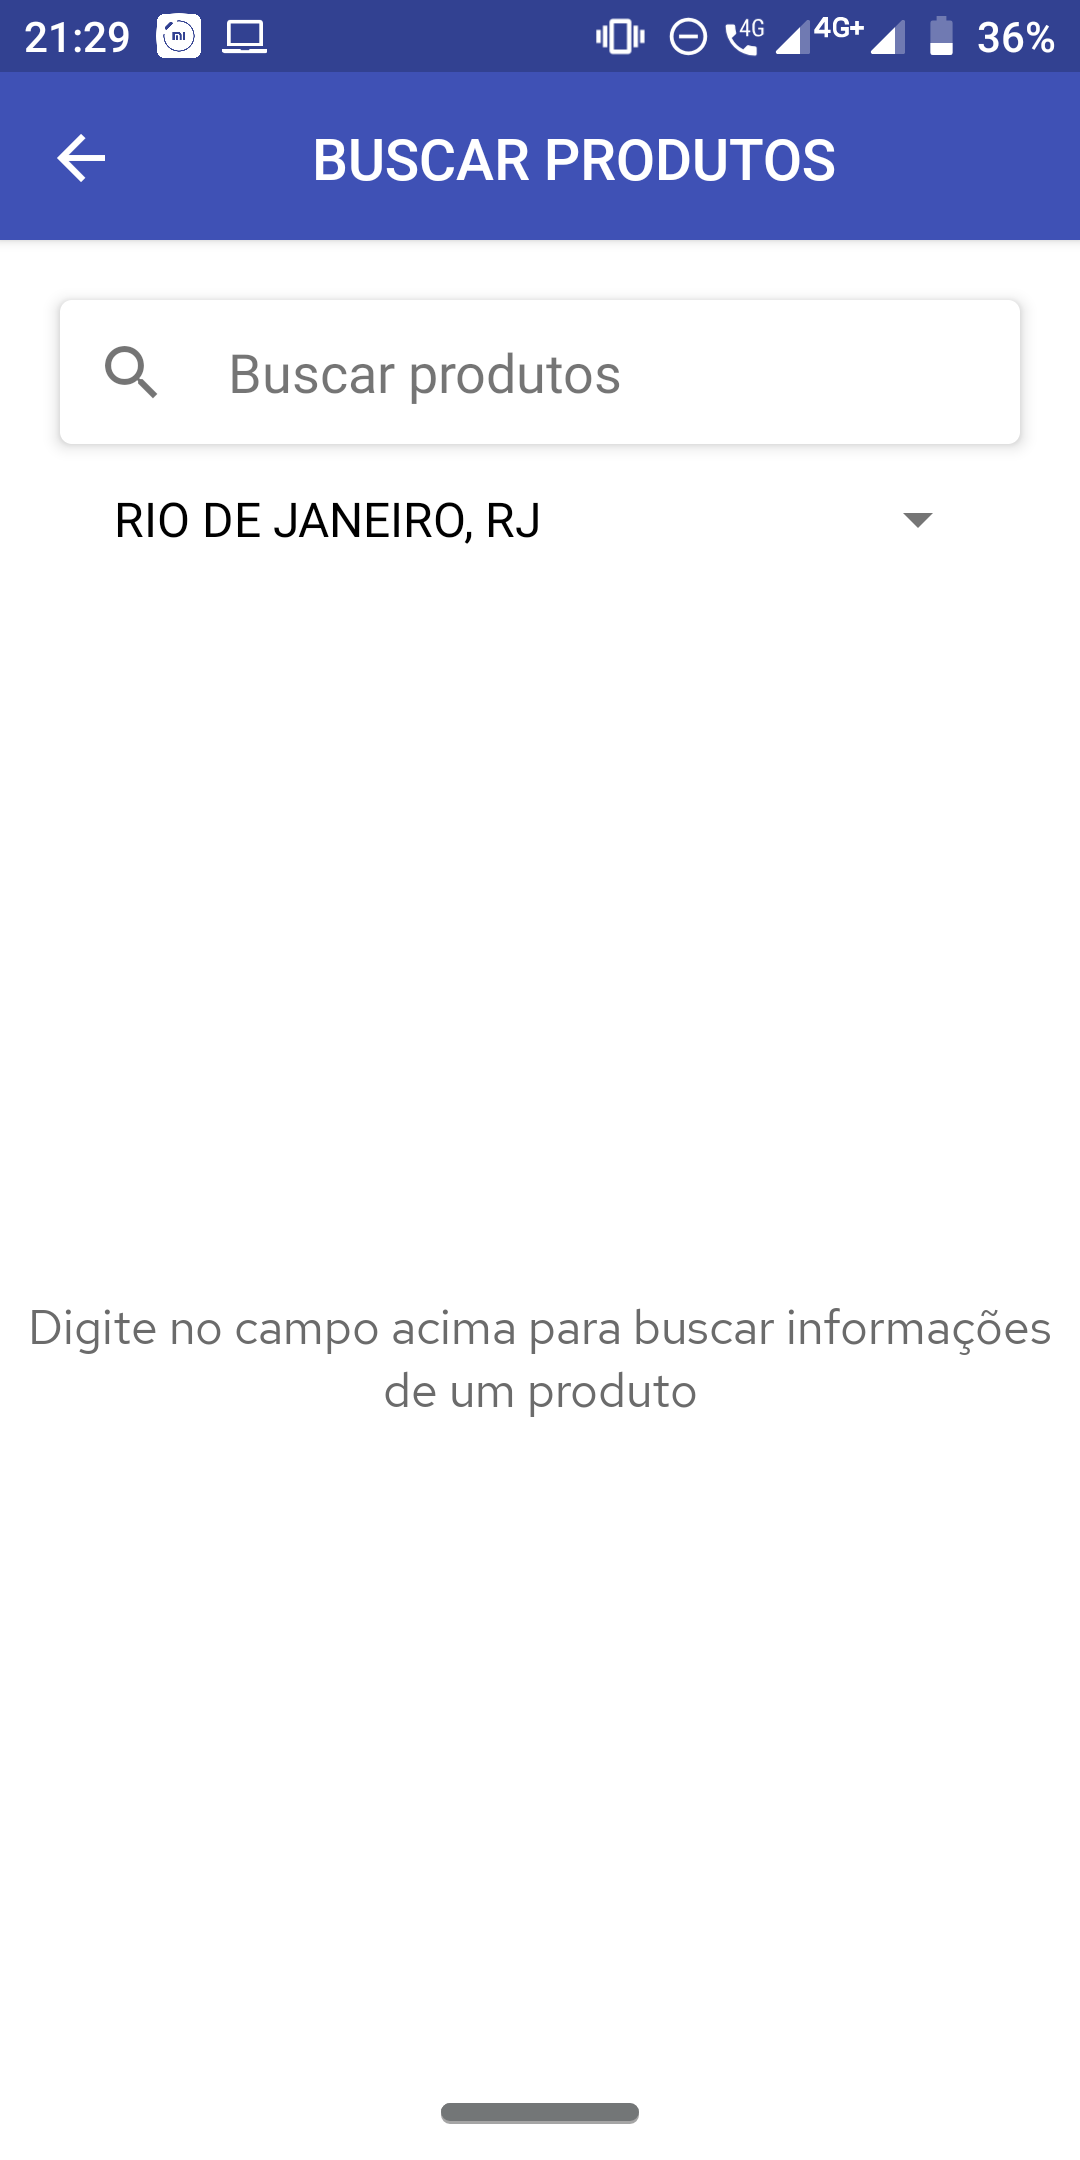
\includegraphics[scale=0.15]{tcc/figures/app/app_buscar_produtos.png}
    \caption{Tela para a realização da busca de produtos}
    \label{appBuscaProdutosInicialFig}
\end{figure}

Logo no início da tela, consta o campo que será utilizado para a inserção do texto referente aos nomes dos produtos. Ao lado esquerdo do campo, existe um ícone no formato de uma lupa que permitirá que o usuário toque para a realização da busca.

Abaixo do campo de texto, existe uma caixa de seleção para que o usuário consulte as cidades disponíveis para busca. Os nomes das cidades são recuperados a partir das notas que foram cadastradas previamente. Além disso, é permitido ao usuário escolher a opção de efetuar a busca em todas as cidades. A figura \ref{appBuscaProdutosCidadesFig} demonstra um exemplo de cidades disponíveis na caixa de seleção para a busca dos produtos.

No meio da tela, constará informações para auxílio ao usuário dependendo da situação em que a tela se encontra. Como pode ser observado na figura \ref{appBuscaProdutosInicialFig}, consta uma breve instrução de como o usuário deve efetuar sua busca. Ademais, caso o produto buscado não seja encontrado na base de dados, nessa mesma área será mostrada a mensagem que os produtos não foram localizados.

% FIXME: Ajustar a imagem
% FIXME: Adicionar referencia a imagem
\begin{figure}[h]
    \centering
    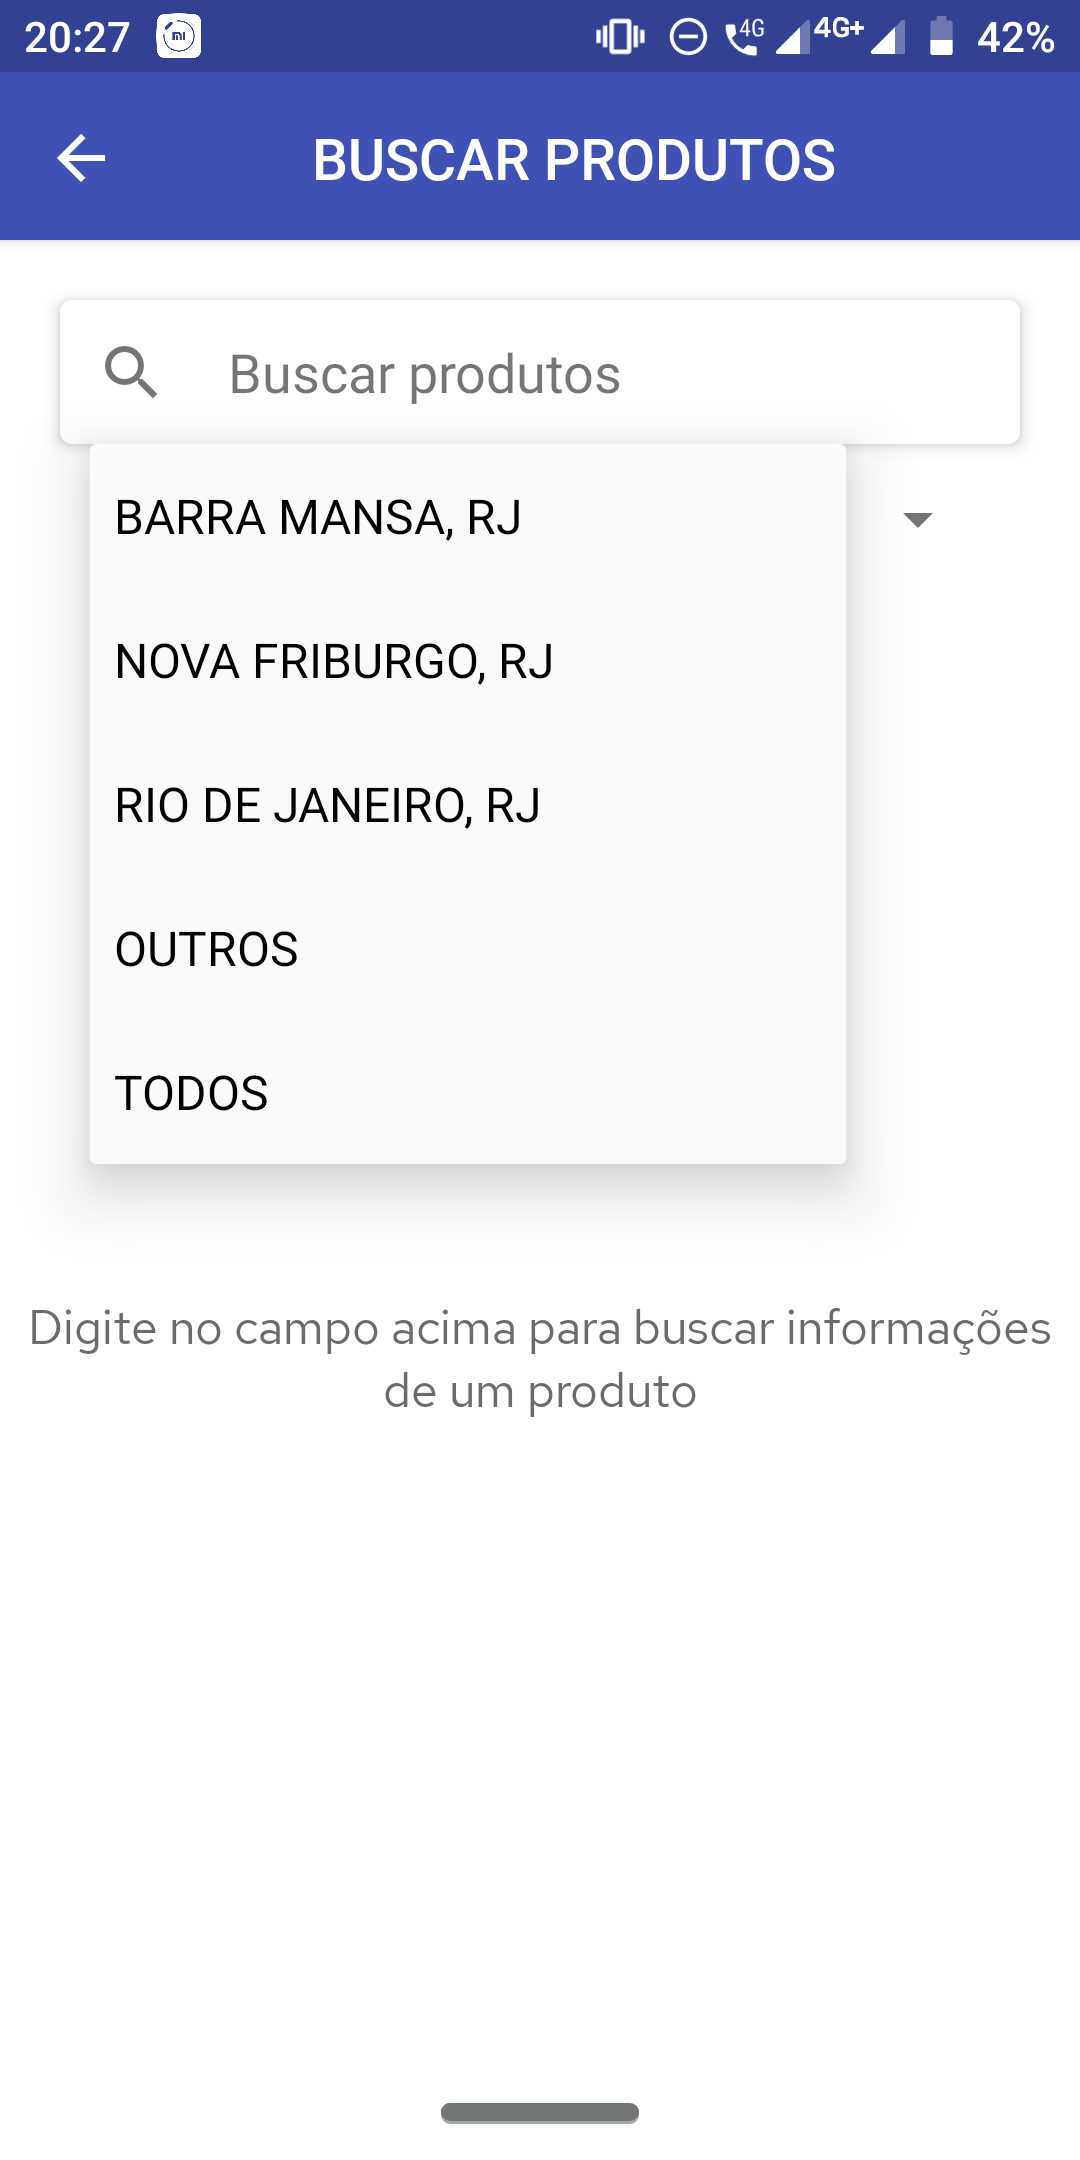
\includegraphics[scale=0.15]{tcc/figures/app/app_buscar_produtos_cidades.png}
    \caption{Exemplo de cidades disponíveis para busca de produtos}
    \label{appBuscaProdutosCidadesFig}
\end{figure}

\newpage
Após a escolha da cidade em que será efetuada a busca, o usuário deverá inserir o nome do produto que deseja buscar no campo de texto dedicado. Vale destacar que o usuário poderá inserir o texto escrito corretamente ou totalmente sem acentuação, e até mesmo com todas as letras em maiúsculo que será retornado o mesmo resultado do cenário em que o usuário escreveu corretamente.

\newpage
% FIXME: Ajustar a imagem
% FIXME: Adicionar referencia a imagem
\begin{figure}[h]
    \centering
    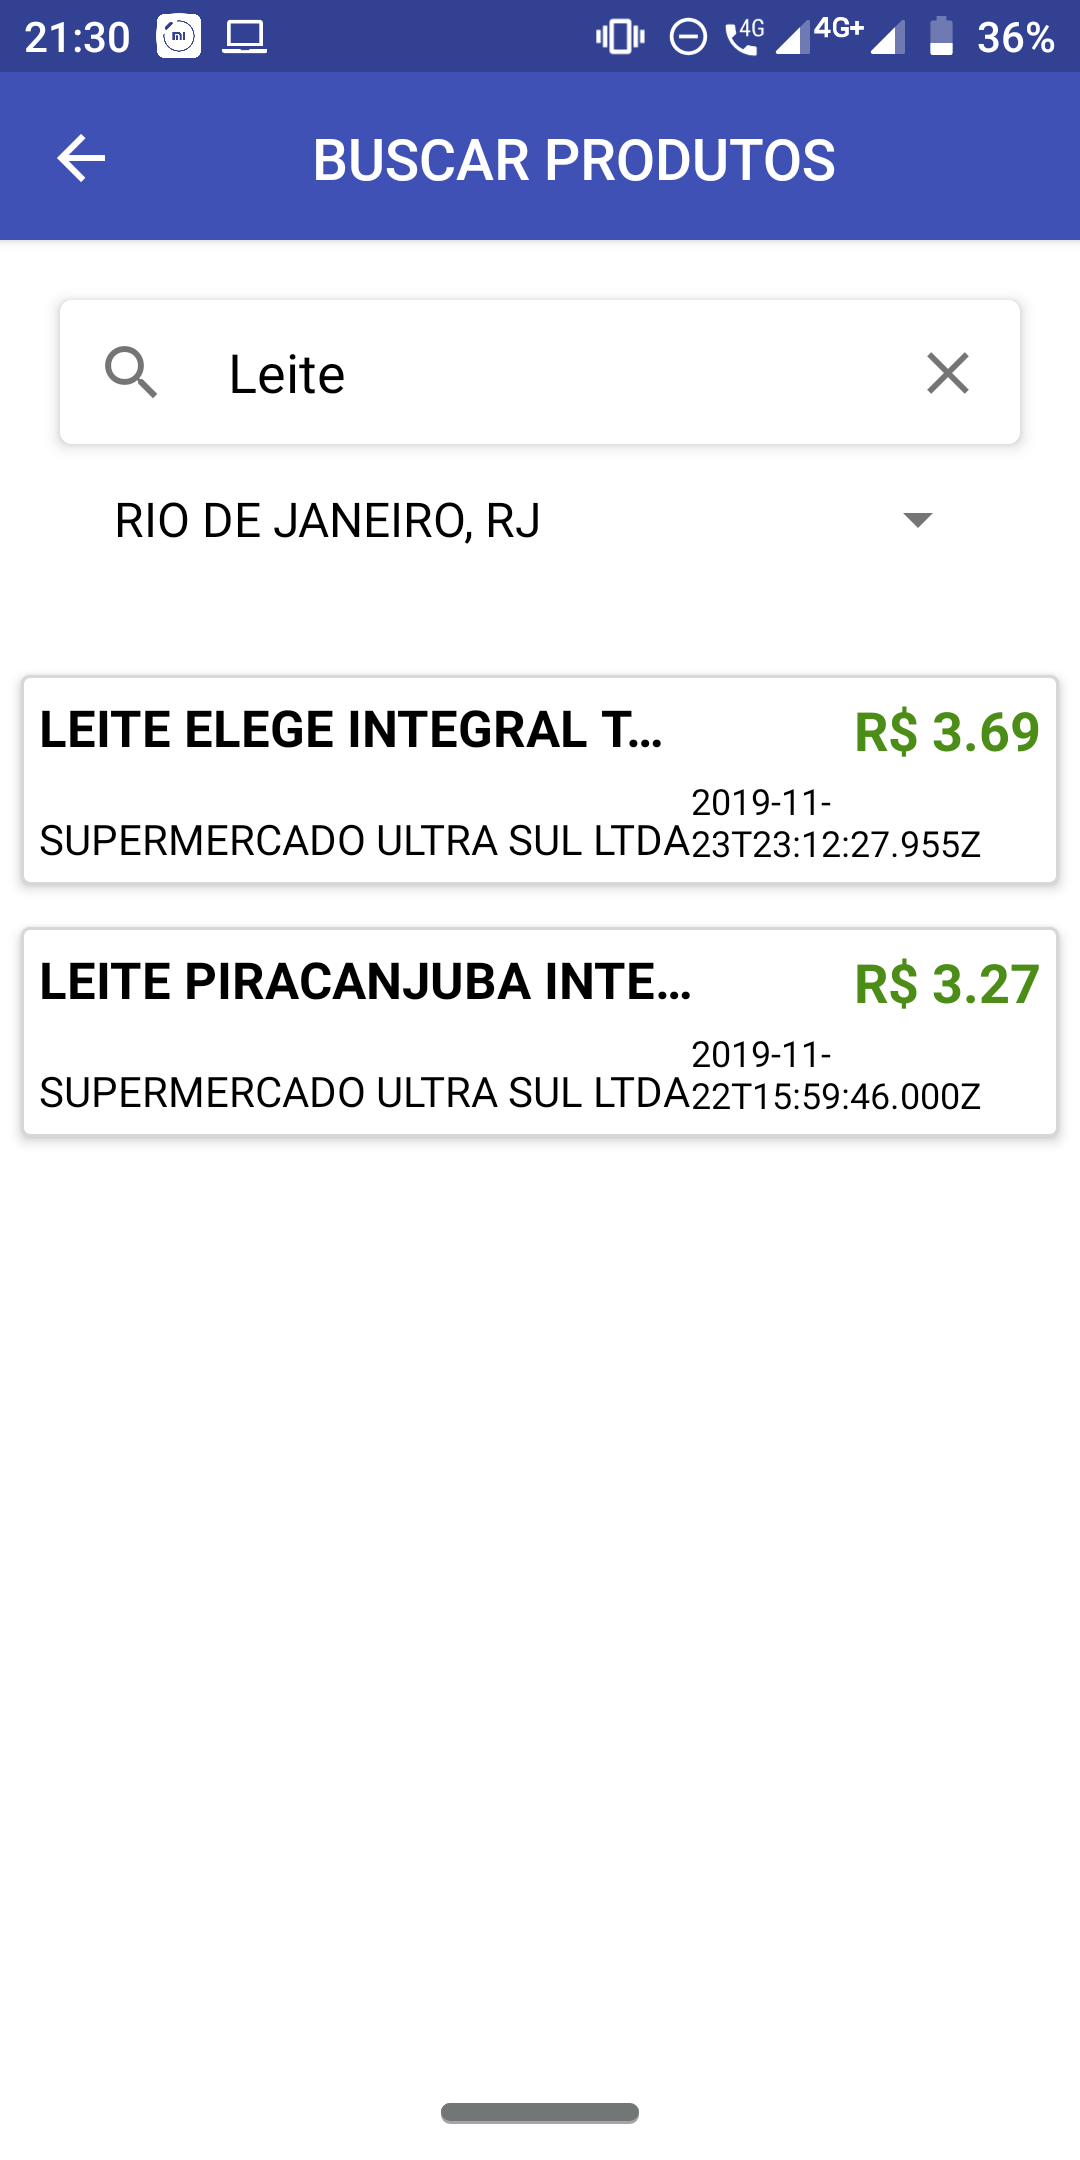
\includegraphics[scale=0.15]{tcc/figures/app/app_buscar_produtos_busca.png}
    \caption{Resultado de uma busca de um produto}
    \label{appBuscaProdutosBuscaResultadoFig}
\end{figure}

Um exemplo de uma busca pelo produto "Leite" é mostrada na figura \ref{appBuscaProdutosBuscaResultadoFig}. Como pode ser observado foram retornados dois registros para esse mesmo produto. Nessa busca, foram encontrados o mesmo produto no entanto de marcas diferentes, além disso, é possível efetuar uma comparação de preços, como também em que dia foi efetuada a compra dos mesmos.

Vale destacar que ambos os produtos foram comprados no mesmo supermercado, no entanto, o nome aparece cortado devido a uma limitação da largura do dispositivo utilizado para efetuar a captura da tela. No entanto, como o nome do mercado pode ser uma cadeia longa de caracteres, esse problema pode ser contornado pois é fornecida uma opção do usuário visualizar as informações completas referentes ao registros individuais dos produtos, para isso, basta efetuar um toque no campo referente ao produto que uma pop-up surgirá em tela contendo as mesmas informações fornecidas anteriormente, no entanto, 
como é possível ocupar a maior parte do espaço disponível em tela, será possível visualizar todas as informações que foram ocultadas anteriormente. Além do nome do local da compra, o próprio nome do produto poderá ser cortado caso esse também seja extenso. Por fim, um exemplo dessa solução descrita anteriormente pode ser observada na figura \ref{appBuscaProdutosProdutoAmpliadoFig}.

% FIXME: Ajustar a imagem
% FIXME: Adicionar referencia a imagem
\begin{figure}[h]
    \centering
    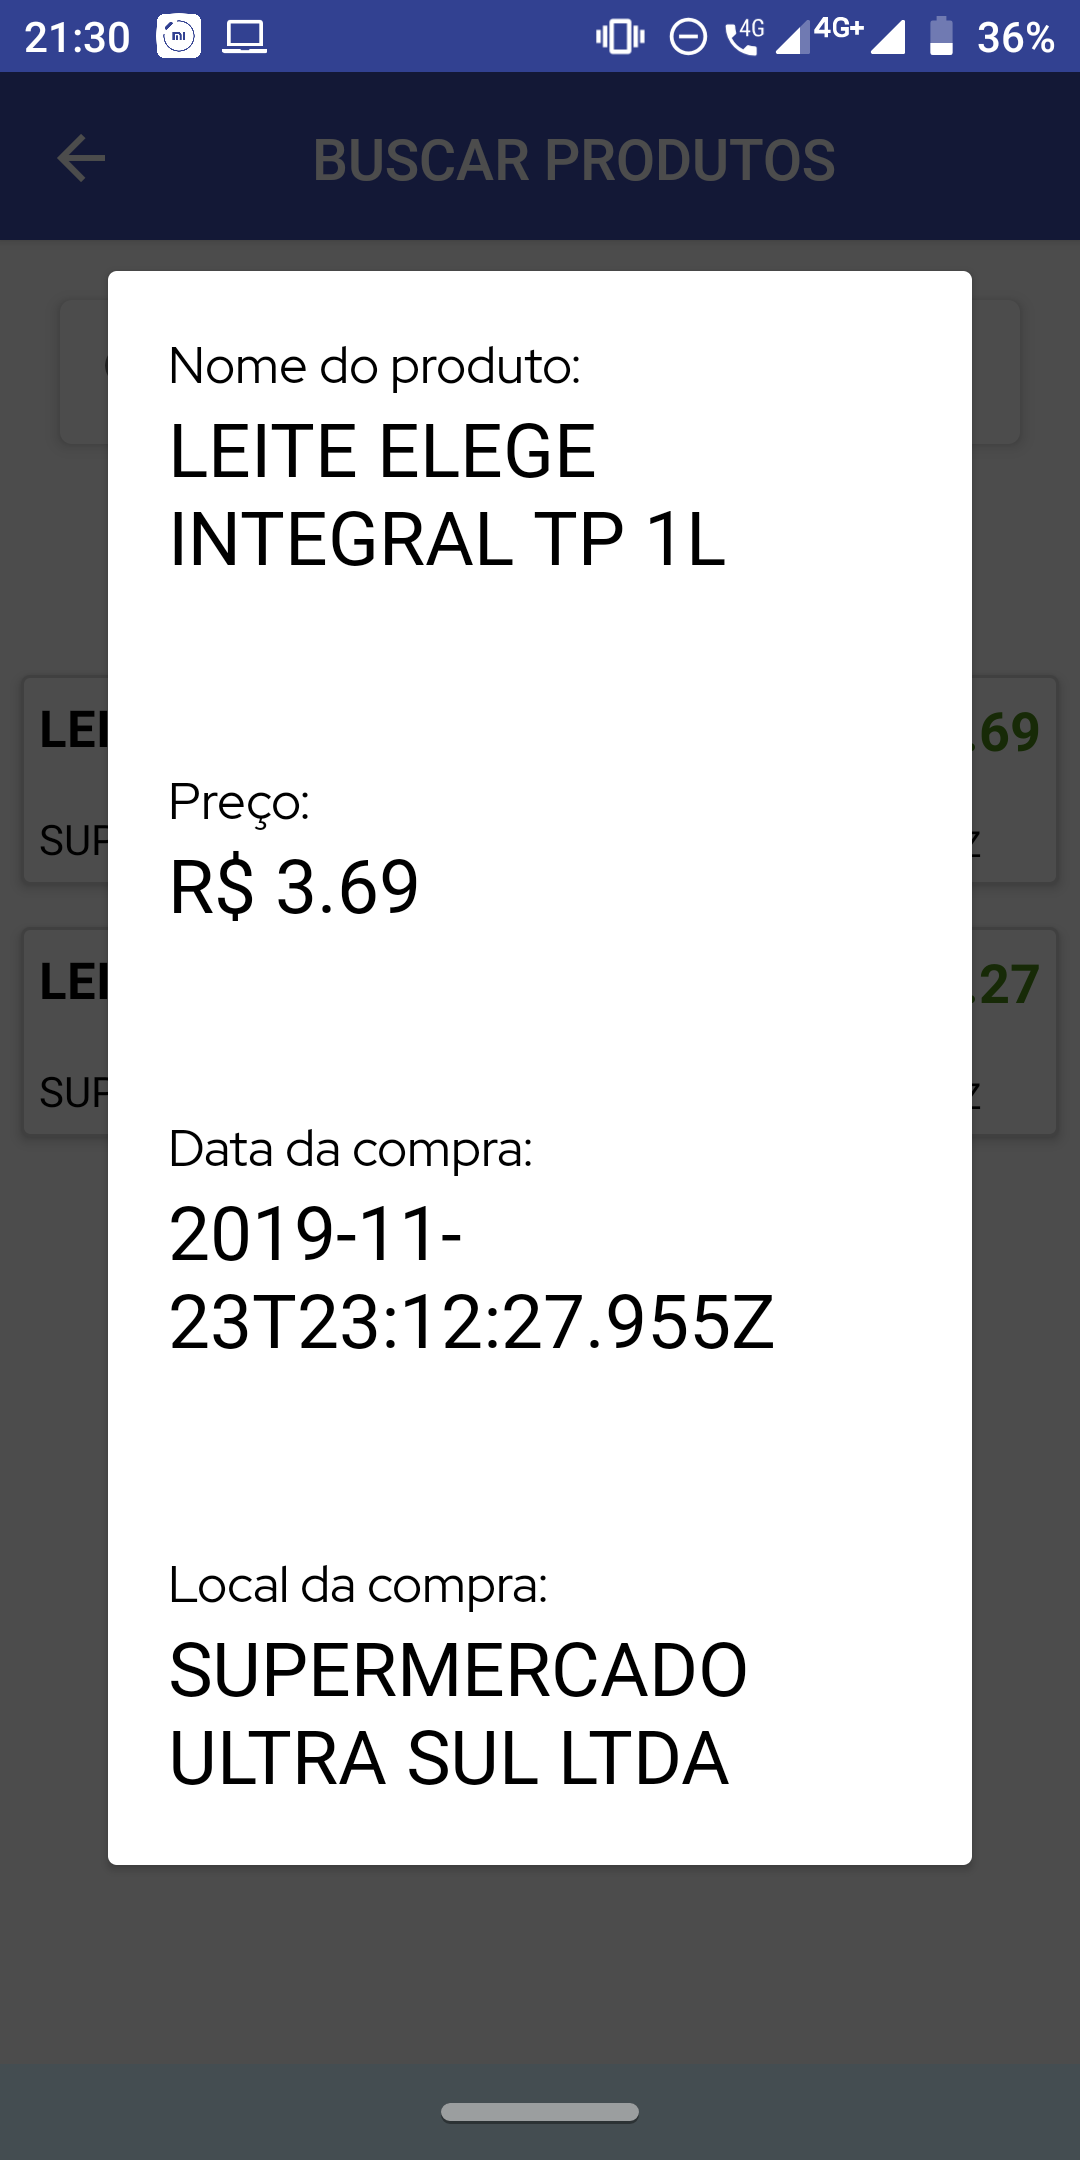
\includegraphics[scale=0.15]{tcc/figures/app/app_buscar_produtos_produto.png}
    \caption{Exemplo de um produto com suas informações disponibilizadas em uma pop-up.}
    \label{appBuscaProdutosProdutoAmpliadoFig}
\end{figure}

\section{Prós e contras do desenvolvimento}

Uma vantagem durante o desenvolvimento, foi que tanto o aplicativo quanto o código do servidor, isto é, a API, foram desenvolvidos utilizando a mesma linguagem de programação, logo, houve uma melhor integração entre as partes.

Alguns problemas ocorreram durante o desenvolvimento da aplicação e da API, como exemplo, pode ser citado que ao efetuar a busca por produtos, todos os produtos contidos na nota fiscal eram retornados. Além disso, durante a busca, a partir do produto não estava sendo possível retornar o local onde o mesmo foi comprado e também, não estava sendo retornando o último registro por mercado, pois estava sempre retornando os registros em que tiveram os menores preços registrados.

Ainda ocorreram problemas durante o desenvolvimento das interfaces da aplicação, pois alguns botões estavam apresentando problemas nas funções que deveriam desempenhar como também o posicionamento dos elementos em tela.

\section{Limitações do aplicativo e das tecnologias utilizadas}

Assim como já foi dito em outros trechos desse trabalho, uma limitação existente na versão atual do aplicativo é que não é possível efetuar a instalação do mesmo a partir das lojas oficias das plataformas suportadas, isto é, a Play Store e a App Store.

Além disso, só é suportado o cadastro de notas fiscais emitidas no Estado do Rio de Janeiro. Ainda relacionado com as notas, o aplicativo apresenta dificuldades de leitura de QRCodes que tiveram problemas durante a impressão.

Por fim, vale observar que o cadastro de notas e a recuperação das informações somente podem ser feitas caso o dispositivo que estiver executando a aplicação esteja conectado à internet.

\subsection{Desvantagem do tipo de banco de dados utilizado}

Uma desvantagem do tipo de banco de dados não-relacional, o qual foi utilizado nesse projeto, é que não foi possui a mesma consistência presente em bancos do tipo relacional, porém, como a informação mais relevante durante a busca dos dados é sempre o último registro efetuado para um produto, logo isso não se torna um problema para o projeto, pois o último registro é sempre garantido.

\section{Obtenção do aplicativo e atualizações}

O autor desse trabalho possui a intenção de efetuar a publicação do aplicativo nas lojas oficias das plataformas suportadas pela aplicação. Conforme, discutido na \autoref{sec-app-desenvolvido}, é possível instalar uma versão funcional do aplicativo, semelhante a que será publicada, em dispositivos que rodam o sistema Android. Vale ressaltar que a prática de instalar aplicativos fora das lojas oficias não é recomendada devido a brechas de segurança. Com isso, o autor se compromete em fornecer um aplicativo seguro que não causará danos ao sistema operacional dos usuários nessa versão prévia do projeto.

Sobre as atualizações com melhorias e correções, poderão ser obtidas de duas formas diferentes, primeiramente dar-se-a através das próprias lojas de aplicativos, após a publicação nas mesmas, já a segunda forma é através do uso de atualizações \textit{Over-the-air} (OTA, em tradução livre: "Por via aérea"), que é um tipo de atualização que o próprio aplicativo efetua o download e realiza a instalação da mesma. Esse recurso é fornecido pela ferramenta Expo e permite que o usuário possua a versão mais atualizada do aplicativo sempre que possível. Por padrão, é efetuada uma verificação por novas atualizações a cada 30 dias. Por fim, por meio dessa última forma é possível ter acesso a versões mais atualizadas do aplicativo sem ser através dos lojas das plataformas.

\section{Disponibilização do código-fonte}

Todo código-fonte desenvolvido para esse trabalho está disponível para acesso através do perfil do autor na plataforma GitHub. Os códigos foram divididos em dois repositórios, um para o desenvolvimento do código a ser executado em servidores e outro para o código referente ao aplicativo.

Através desses repositórios, novas funcionalidades poderão ser adicionadas pela comunidade de desenvolvedores como também o desenvolvimento de novos projetos tendo como base esse trabalho aqui desenvolvido. Os repositórios podem ser acessados através dos seguintes endereços:
\begin{itemize}
\item Servidor: https://github.com/gav1ao/market-api;
\item Aplicativo: https://github.com/gav1ao/market-mobile;
\end{itemize}

Esses mesmos endereços também podem ser acessados através dos seguintes QRCodes disponibilizados logo abaixo:

% FIXME: Ajustar a imagem
% FIXME: Adicionar referencia a imagem
\begin{figure}[h]
    \centering
    
\includegraphics[scale=0.5]{tcc/figures/repo_qrcode/repo_github_market_api.png}
    \caption{Link para o repositório do servidor}
    \label{fig-repo-qrcode-api}
\end{figure}

% FIXME: Ajustar a imagem
% FIXME: Adicionar referencia a imagem
\begin{figure}[h]
    \centering
    
\includegraphics[scale=0.5]{tcc/figures/repo_qrcode/repo_github_market_app.png}
    \caption{Link para o repositório do servidor}
    \label{fig-repo-qrcode-app}
\end{figure}

	\chapter{Cap. 5}

\lipsum

	% Elementos pós-textuais
	\postextual
	%\include{glossario}
	\apendices

\chapter{Primeiro apêndice}
Primeiro apêndice!

\chapter{Segundo apêndice}
Segundo apêndice
	\anexos

\chapter{Primeiro anexo}
Primeiro anexo!

\chapter{Segundo anexo}
Segundo anexo!
	% a abntex2-cite nao aceita o comando \nocite{*}
% portanto cada referencia nao citada deve ser
% adicionada aqui para constar na bibliografia

%\nocite{abnt-classe-doc}

% \nocite{abntex2classe}
% \nocite{abnt-bibtex-doc}
% \nocite{abnt-bibtex-alf-doc}
% \nocite{abnt-classe-doc}
% \nocite{tabela-simbolos-doc}
% \nocite{knuth}
% \nocite{lamport}
% \nocite{lrparsing}
% \nocite{intautomata}
% \nocite{inttheory}
% \nocite{contextfreel}
% \nocite{Kaltofen82factorizationof}
% \nocite{algebramoresym}
% \nocite{elementaryalg}
% \nocite{mathmethods}
% \nocite{symbc}
% \nocite{appliedaero}
% \nocite{cursocalculo}
% \nocite{languagechange}
% \nocite{structureint}
% \nocite{Bartholomew-Biggs2000ADo}
% \nocite{cidoribeiro}
% \nocite{educmat}
% \nocite{useeducation}
% \nocite{precedence}
% \nocite{intautdiff}
% \nocite{autdifftech}
% \nocite{evalderivatives}
% \nocite{modernalgebra}
% \nocite{algalgebra}

\nocite{edirlei2015}
\nocite{fischerGrodzinsky1993}
\nocite{iphoneApple}
\nocite{tiobeAbout}
\nocite{tiobeDefinition}
\nocite{stackOverflowAbout}
\nocite{stackOverflowRanking}
\nocite{qrCodeCanalTech}
\nocite{qrCodeOlharDigital}

\nocite{captchaGoogle}
\nocite{captchaG1}
\nocite{captchaExame}
\nocite{captchaTecmundo}
\nocite{captchaWikipedia}

\nocite{nfceDefinicao}

\nocite{desenvolvimentoMobile}
\nocite{xamarimDefinicao}

\nocite{nodeJsSobre}
\nocite{nodeJsMDN}
\nocite{angularIntroduction}
\nocite{angularWiki}
\nocite{vueJsAbout}
\nocite{vueJsWiki}
\nocite{reactAbout}
\nocite{reactWiki}
\nocite{reactNativeAbout}
\nocite{reactNativeWiki}

\nocite{silberschatz2016sistema}

\nocite{cheerio}
\nocite{heroku}
\nocite{githubStudentPack}
\nocite{webscrapingRockContent}
\nocite{pixDefinicao}
\nocite{mobileDatabase}
\nocite{menorPrecoApp}
\nocite{pinngoApp}
\nocite{meusPrecosApp}
\nocite{melhorPrecoAmazonasApp}

\nocite{mongoDBDefinition}
\nocite{flutterDefinition}
\nocite{beautifulSoupDefinition}
\nocite{jSoupDefinition}
\nocite{jSoupAndroid}
\nocite{expo}
\nocite{expoOverview}
\nocite{inflacaoEstadoMinas}
\nocite{inflacaoEstadao}
\nocite{blackFridayVeja}
\nocite{tiposBancoDeDados}
\nocite{sqLite}
\nocite{javascriptHistoria}
\nocite{formValidation}
\nocite{javascriptWikipedia}
	\bibliography{tcc}
\end{document}